\documentclass[12pt,letterpaper,oneside,openany,spanish]{book}
\usepackage{newtxtext,newtxmath}
\usepackage[utf8]{inputenc}
\usepackage[spanish]{babel}
\usepackage{graphicx}
\usepackage{amsmath} 
\usepackage{hyperref}
\usepackage{listings}
\usepackage[dvipsnames,table,xcdraw]{xcolor}
\usepackage{courier}
\usepackage{geometry}
\usepackage{changepage}
\usepackage{titlesec}
\usepackage{wrapfig}
\usepackage[version=4]{mhchem}
\usepackage{multirow}
\usepackage{siunitx}
\usepackage{tikz}
\usepackage{epigraph}
\usepackage{titlesec}
\usepackage{ragged2e}
\usepackage{multicol}
\usepackage{float}
\usepackage{pdfpages}
\usepackage{csquotes}
\usepackage{array}
\usepackage[shortlabels]{enumitem}


%%%%%%%%%%%%%%%%%%%%%%%%%%%%%%%%%%%%%%%%%%%%%
%%%%%%%%%%%      importante     %%%%%%%%%%%%%
%%%%%%%%%%%%%%%%%%%%%%%%%%%%%%%%%%%%%%%%%%%%%
% hay que darle a menú, y escoger el compilador "LuaLaTeX"

\renewcommand\epigraphflush{flushright}
\renewcommand\epigraphsize{\normalsize}
\setlength\epigraphwidth{0.7\textwidth}

\pagenumbering{arabic}

%cosas para los margenes
\newenvironment{changemargin}[2]{%
\begin{list}{}{%
\setlength{\topsep}{0pt}%
\setlength{\leftmargin}{#1}%
\setlength{\rightmargin}{#2}%
\setlength{\listparindent}{\parindent}%
\setlength{\itemindent}{\parindent}%
\setlength{\parsep}{\parskip}%
}%
\item[]}{\end{list}}


% Quita el título 'Capítulo N' a cada capítulo
\titleformat{\chapter}[display]{\normalfont\bfseries}{}{0pt}{\Huge}
\newpagestyle{mystyle}
% Quita el header con 'capítulo n: blablabla'
{\sethead[\thepage][][\chaptertitle]{}{}{\thepage}}
\pagestyle{mystyle}

% Cosas de la portada fancy
\definecolor{titlepagecolor}{cmyk}{1,.60,0,.40}

\DeclareFixedFont{\titlefont}{T1}{ppl}{b}{it}{0.6in}

\makeatletter                       
\def\printauthor{                  
    {\large \@author}}              
\makeatother
% Autores
\author{
    Lucía Selena Sarasty Bolaños \\
    \texttt{48775044W}\vspace{20pt} \\
    Víctor Mira Ramírez \\
    \texttt{74528754Z}
    }

\newcommand\titlepagedecoration{
    \begin{tikzpicture}[remember picture,overlay,shorten >= -10pt]
    
    \coordinate (aux1) at ([yshift=-15pt]current page.north east);
    \coordinate (aux2) at ([yshift=-410pt]current page.north east);
    \coordinate (aux3) at ([xshift=-4.5cm]current page.north east);
    \coordinate (aux4) at ([yshift=-150pt]current page.north east);
    
    \begin{scope}[titlepagecolor!40,line width=12pt,rounded corners=12pt]
    \draw
      (aux1) -- coordinate (a)
      ++(225:5) --
      ++(-45:5.1) coordinate (b);
    \draw[shorten <= -10pt]
      (aux3) --
      (a) --
      (aux1);
    \draw[opacity=0.6,titlepagecolor,shorten <= -10pt]
      (b) --
      ++(225:2.2) --
      ++(-45:2.2);
    \end{scope}
    \draw[titlepagecolor,line width=8pt,rounded corners=8pt,shorten <= -10pt]
      (aux4) --
      ++(225:0.8) --
      ++(-45:0.8);
    \begin{scope}[titlepagecolor!70,line width=6pt,rounded corners=8pt]
    \draw[shorten <= -10pt]
      (aux2) --
      ++(225:3) coordinate[pos=0.45] (c) --
      ++(-45:3.1);
    \draw
      (aux2) --
      (c) --
      ++(135:2.5) --
      ++(45:2.5) --
      ++(-45:2.5) coordinate[pos=0.3] (d);   
    \draw 
      (d) -- +(45:1);
    \end{scope}
    \end{tikzpicture}
}



\begin{document}
\begin{titlepage}

% Texto de la portada
\noindent
\titlefont Informes Química I\par

\epigraph{\vspace{1cm} \justify Síntesis de todas las prácticas de laboratorio realizadas en el curso 2021-22 en la asignatura Química I del grado en Física de la Universidad de Alicante.}
{\textit{Profesor: Jesús Iniesta Valcárcel} \\ \textit{Alicante, 2022}}
\null\vfill
\vspace*{1cm}
\noindent
\hfill
\begin{minipage}{0.4\linewidth}
    \begin{flushright}
        \printauthor
    \end{flushright}
\end{minipage}
\hspace*{-0.2cm}
\begin{minipage}{-0.2\linewidth}
    \rule{1pt}{100pt}
\end{minipage}
\titlepagedecoration
\end{titlepage}

\clearpage
\pagenumbering{gobble}
\tableofcontents
\clearpage

%%%%%%%%%%%%%%%%%%%%%%%%%%%%%%%%%%%%%%%%%%%
%%%%%%%%%%%     PRÁCTICAS     %%%%%%%%%%%%%
%%%%%%%%%%%%%%%%%%%%%%%%%%%%%%%%%%%%%%%%%%%

% Recordatorio: solo hay q escribir en los archivos prN.tex, en el main no hay que cambiar nada a menos q queramos poner fotos en la portada


% PRÁCTICA 1
\pagenumbering{arabic}
\setcounter{page}{4}
    \chapter[Práctica 1]{1. Preparación de disoluciones y de la concentración de ácido cítrico, \ce{C8H8O7}}
    \thispagestyle{empty}
    \vspace{1cm}
    \begin{figure}[h]
        \centering
        \hspace*{-0.2cm}
        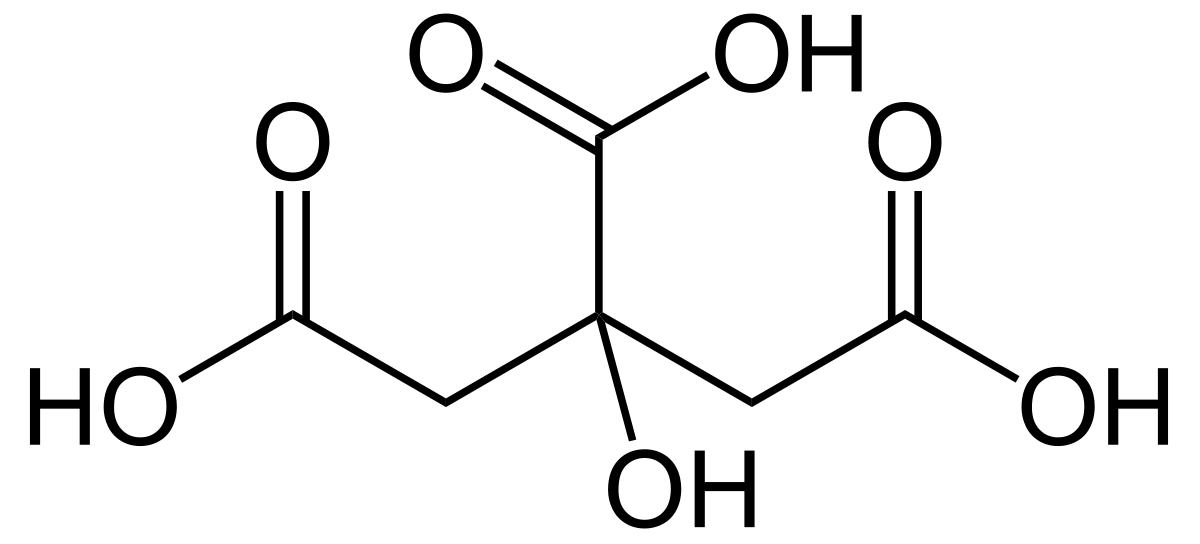
\includegraphics[width=.48\textwidth]{fotos/citrico.png}\hfill
        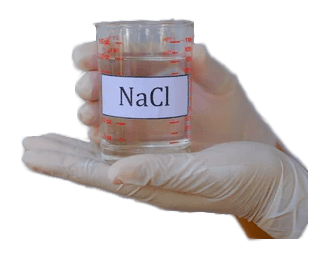
\includegraphics[width=.48\textwidth]{fotos/disolucion.png}
        \hspace*{-0.4cm}
    \end{figure}
\section{Introducción}  %y he visto que boris puso que tb resumen
    \noindent En esta práctica prepararemos varias disoluciones de  \ce{NaCl} con agua a partir de una disolución inicial. Se nos proporcionarán las especificaciones de dichas sdisoluciones (es decir, su concentración) de formas diferentes: su molaridad, molalidad o porcentaje en masa.
    \\ \\Primeramente, de estas disoluciones obtendremos valores para sus densidades utilizando métodos distintos explicados en el laboratorio (picnómetro y aerómetro) electromagnético. En una segunda parte determinaremos la concentración de ácido cítrico (\ce{C6H8O7}) de una disolución problema, realizando una valoración de la misma usando un indicador (fenolftaleína (\ce{C20H14O4})) y una base (Hidróxido de sodio(\ce{NaOH})).

\section{Inventario}
\noindent Para esta práctica hemos usado:

\begin{multicols}{2}
    \begin{itemize}
        \item Aerómetro de $30 ml$
        \item Aerómetro de $10 ml$
        \item Picnómetro
        \item Pesa electrónica
        \item Bandeja pequeña
        \item Espátula metálica
        \item Bureta
        \item 2 Pipetas
        \item 2 Propietas
        \item 4 Matraces aforados
    \end{itemize}
\end{multicols}

\begin{figure}[H]
    \centering
    \includegraphics[width=.4\textwidth]{prac1/aerómetros.jpg}\hfill
    \includegraphics[width=.4\textwidth]{prac1/picnómetro.jpg}
    \caption{A la izquierda aerómetros y a la derecha un picnómetro}
    \vspace{-1cm}
\end{figure}

\clearpage

\section{Procedimiento}
\subsection{Preparación de disoluciones}
\noindent En esta parte de la práctica vamos a preparar cuatro disoluciones distintas de \ce{NaCl} cada una de ellas con procedimientos distintos. A la primera de ellas la llamaremos A y será una disolución del 20\% en masa. A partir de esta primera disolución haremos las otras 3. La B será una disolución al 5\%, la C 1 molar y la D 1 molal.\\\\
Una vez prepradas, calcularemos la densidad de la disolución A mediante el uso de un picnómetro y obtenemos una densidad de $1.1422 \si{g/ml}$.\\\\
\noindent El valor de la densidad de la disolución A obtenido con el picnómetro se consiguió gracias esta expresión:
\[\rho = \rho_{\ce{H2O}}\cdot\frac{m_{\text{pic + dis}}-m_{\text{pic}}}{m_{\text{pic + \ce{H2O}}}-m_{\text{pic}}}\]
\noindent Finalmente, medimos la densidad de las cuatro disoluciones obtenidas mediante el método del aerómetro. Para este méetodo, hemos de tener en cuenta que el resultado nos quedará en grados Baumé, los cuales convertiremos en \si{g/ml} con la siguiente fórmula:
\[Be = 145-\frac{145}{\rho}\]
\noindent En la siguiente tabla se recogen las medidas de la densidad realizadas con el aerómetro para cada disolución.\\
\begin{table}[H]
\centering
\begin{tabular}{ccc}
\rowcolor[HTML]{9698ED} 
\textbf{Disolución} & \textbf{Aerómetro} & \textbf{g/ml} \\
\rowcolor[HTML]{DAE8FC} 
\textbf{A} & $18.3$ & $1.444$ \\
\textbf{B} & $5$ & $1.036$ \\
\rowcolor[HTML]{DAE8FC} 
\textbf{C} & $5.6$ & $1.040$ \\
\textbf{D} & $5.5$ & $1.039$
\end{tabular}
\caption{Densidades}
\label{densidades}
\end{table}
\vspace{0.2cm}
\noindent Observamos como el método del picnómetro y el del aerómetro se aproximan notoriamente. Concluimos que usar el aerómetro para medidas aproximadas es más eficiente gracias a una inversión temporal menor en la realización de las medidas.

\clearpage
\subsection{Determinación de la concentración de ácido cítrico}
\noindent En primer lugar, pipeteamos 1 \si{mL} de la disolución problema de ácido cítrico (X) y se vierte en un matraz Erlenmeyer limpio. A continuación, se homogeneiza la bureta con una pequeña cantidad de disolución patrón (P) de \ce{NaOH} 0.10M. Seguidamente, añadimos tres gotas de fenolftaleína en el matraz.\\\\ 
En el momento en el que el líquido del matraz adquiera una coloración diferente (en este caso rosácea) y permanente se cierra por completo la llave de la bureta y anotamos el volumen de la disolución de \ce{NaOH} (P) gastado en el proceso en el siguiente cuadro:\\

\begin{table}[H]
\centering
\begin{tabular}{cc}
\rowcolor[HTML]{9698ED} 
\textbf{Muestra} & \textbf{V(\si{ml})} \\
\rowcolor[HTML]{DAE8FC} 
1 & $10.2$ \\
2 & $10.2$ \\
\rowcolor[HTML]{DAE8FC} 
3 & $10.2$ \\
 &  \\
\rowcolor[HTML]{FCFF2F} 
Media & $10.2$
\end{tabular}
\caption{Valoración}
\label{valoracin}
\end{table}
\vspace{0.4cm}

\noindent Esta es la reacción que está sucediendo en la valoración del ácido cítrico:
\[\ce{C3H4OH(COOH)3 + 3NaOH -> C3H4OH(COONa)3 + 3H2O}\]
\clearpage

\section{Cuestiones}
\vspace{0.4cm}
\noindent\textcolor{BlueViolet}{\textbf{\textit{a) Calcule la concentración de cada una de las disoluciones A, B, C y D en las 10 formas descritas en la introducción y resuma los resultados en una tabla.}}}\\\\
\noindent En esta cuestión se nos pide calcular la concentración de nuestras disoluciones siguiendo los diversos métodos que se exponen en el guión. A partir de los datos obtenidos del \textquote{\textit{CRC Handbook of Chemistry and Physics}} (es decir, que $\rho_{\text{agua}} = 0.9982\ \si{g/ml}$) quedan los cálculos de los diez métodos resumidos en la siguiente tabla:\\

\begin{table}[H]
\renewcommand{\arraystretch}{1.9}
\centering
\newcolumntype{A}{ >{}m{4cm} }
\newcolumntype{B}{ >{\centering\arraybackslash} m{2.4cm} }
\newcolumntype{C}{ >{\centering\arraybackslash} m{1.3cm} }
\resizebox{\textwidth}{!}{
\begin{tabular}{A B C C C C}
 &  & \cellcolor[HTML]{9698ED}\textbf{A} & \cellcolor[HTML]{9698ED}\textbf{B} & \cellcolor[HTML]{9698ED}\textbf{C} & \cellcolor[HTML]{9698ED}\textbf{D} \\
\rowcolor[HTML]{ECF4FF} 
\cellcolor[HTML]{9698ED}\textbf{Molaridad \small{(\si{M})}} & \cellcolor[HTML]{9698ED}\textbf{$\frac{n_{\text{soluto}}}{\si{L}_{\text{disolución}}}$} & $4$  & $0.5$ & $1$ &  $0.9$\\
\cellcolor[HTML]{DAE8FC}\textbf{Molalidad \small{(\si{m})}} & \cellcolor[HTML]{DAE8FC}\textbf{$\frac{n_{\text{soluto}}}{\si{kg}_{\text{disolvente}}}$} & $4.3$ & $0.6$ & $1$ & $1$ \\
\rowcolor[HTML]{ECF4FF} 
\cellcolor[HTML]{9698ED}\textbf{Fracción molar} & \cellcolor[HTML]{9698ED}\textbf{$\frac{n_{\text{soluto}}}{n_{\text{totales}}}$} & $0.074$ & $0.0015$ & $0.0181$ & $0.016$ \\
\cellcolor[HTML]{DAE8FC}\textbf{Razón molar} & \cellcolor[HTML]{DAE8FC}\textbf{$\frac{n_{\text{soluto}}}{n_{\text{disolvente}}}$} & $0.08$ &  $0.015$ &  $0.0184$ & $0.017$ \\
\rowcolor[HTML]{ECF4FF} 
\cellcolor[HTML]{9698ED}\textbf{Fracción másica} & \cellcolor[HTML]{9698ED}\textbf{$\frac{\si{g}_{\text{soluto}}}{\si{g}_{\text{disolución}}}$} & $0.2$ & $0.05$ & $0.06$ & $0.05$ \\
\cellcolor[HTML]{DAE8FC}\textbf{Razón másica} & \cellcolor[HTML]{DAE8FC}\textbf{$\frac{\si{g}_{\text{soluto}}}{\si{g}_{\text{disolvente}}}$} & $0.25$ &$0.53$ & $0.06$ & $0.059$ \\
\rowcolor[HTML]{ECF4FF} 
\cellcolor[HTML]{9698ED}\textbf{Porcentaje en peso} & \cellcolor[HTML]{9698ED}\textbf{$\frac{\si{g}_{\text{soluto}}}{\si{g}_{\text{disolución}}} \cdot 100$} & $20\%$ & $5\%$ & $6\%$ & $5\%$ \\
\cellcolor[HTML]{DAE8FC}\textbf{Gramos por litro \small{(\si{g/L})}} & \cellcolor[HTML]{DAE8FC}\textbf{$\frac{\si{g}_{\text{soluto}}}{\si{L}_{\text{disolución}}}$} & $250$ & $52$ & $58$ & $0.058$ \\
\rowcolor[HTML]{ECF4FF} 
\cellcolor[HTML]{9698ED}\textbf{Partes por millón} & \cellcolor[HTML]{9698ED}\textbf{$\frac{\si{g}_{\text{soluto}}}{\si{g}_{\text{disolución}}} \cdot 10^6$} & $2\cdot10^5$ & $5\cdot10^4$ & $6\cdot10^4$ & $4.2\cdot10^4$ \\
\cellcolor[HTML]{DAE8FC}\textbf{Partes por billón} & \cellcolor[HTML]{DAE8FC}\textbf{$\frac{\si{g}_{\text{soluto}}}{\si{g}_{\text{disolución}}} \cdot 10^9$} & $2\cdot10^8$ & $5\cdot10^7$ & $6\cdot10^7$ & $5.2\cdot10^7$
\end{tabular}
}
\end{table}
\vspace*{-2cm}

\clearpage

\noindent\textcolor{BlueViolet}{\textbf{\textit{b) Se quiere preparar una disolución de carbonato sódico al 8\% en peso, partiendo de la sal decahidratada. Calcule las cantidades de sal hidratada y de agua que son necesarias.}}}\\

\noindent Primero ajustamos la ecuación que se nos pide:
\[\ce{20H2O\cdot NaCl + H2CO3 -> Na2CO3 + 2HCl + 20H2O}\]
\noindent Suponiendo que se generan 100\si{g} de \ce{Na2CO3} impuros, obtenemos la formación de 8\si{g} de \ce{Na2CO3} puro. Con el siguiente factor de conversión concluimos los moles necesarios para la obtención de 8g puros:
\[ 8\si{g}\ \ce{Na2CO3} \cdot \frac{1\ce{mol}\ \ce{Na2CO3}}{2\cdot23\si{g}\ \ce{Na}\ +\ 3\cdot16\si{g}\ \ce{O}} \cdot \frac{2\si{mol}\ \ce{H2O}\cdot\ce{NaCl}}{1\si{mol}\ \ce{Na2CO3}} = 0.151\ \si{mol}\ \ce{H2O}\cdot\ce{NaCl}\]\\\\\\
\noindent\textcolor{BlueViolet}{\textbf{\textit{c) Se quiere preparar 100 mL de una disolución de hidróxido sódico 0,2 M. Calcule la cantidad de hidróxido sódico y de agua que son necesaria para preparar la disolución.}}}\\

\noindent En esta cuestión se nos pide calcular la cantidad de hidróxido de sodio (\ce{NaOH}) y agua (\ce{H2O}) necesarios para obtener una disolución $0.2 M$. A partir de la fórmula de la cuestión 1 ($M = \frac{n_{soluto}}{\si{L}_{disolución}}$) haremos el siguiente factor de conversión y obtendremos la respuesta:

\[100\si{ml} \ \ce{NaOH} \cdot \frac{1\si{L}}{1000\si{ml}} \cdot \frac{0.2 \si{mol} \ \ce{NaOH}}{1 \si{L}\ \text{disolución}} = 0.02 \si{mol} \ \ce{NaOH}\]\\\\\\
\noindent\textcolor{BlueViolet}{\textbf{\textit{d) Calcule, a partir del resultado de la valoración la concentración de ácido cítrico problema.}}}\\

\noindent Primero, como sabemos la molaridad de la disolución que tenemos de NaOH,
calculamos los moles que tenemos que serán 0,0011 moles de NaOH y como por
estequiometria de la reacción que se produce, sabemos que la relación es 3 mol
NaOH/mol C6H8O7, llegamos a que tenemos 0,0033 moles de C6H8O7 y por tanto la
molaridad de la disolución que tenemos es 0,33 M.

% PRÁCTICA 2
\chapter[Práctica 2]{2. Termoquímica}
\thispagestyle{empty}
\vspace{1cm}
\begin{figure}[h]
    \centering
    \hspace*{-0.2cm}
    \includegraphics[width=.8\textwidth]{fotos/portada.jpg}
    \hspace*{-0.4cm}
    \end{figure}
\section{Introducción}  %RESUMEEEEN
\noindent En esta practica realizaremos diversas mezclas para determinar su carácter (exotérmico o endotérmico), así como determinaremos el equivalente en agua del calorímetro usando para ello agua destilada tanto fría como caliente. Y por último, determinaremos la entalpía de neutralización tanto de un ácido fuerte con una base fuerte como un ácido débil con una base fuerte.

\section{Inventario}
Para esta práctica hemos usado:

\begin{multicols}{2}
    \begin{itemize}
        \item Un calorímetro
        \item Una pipetas graduadas
        \item Una propipeta
        \item Un termómetro
        \item 4 tubos de ensayo
        \item 2 vasos de precipitados
        \item 2 pipetas pasteur
        \item Una varilla
        \item 2 espátulas
        \item 2 probetas
        \item Un recipiente negro para pesar diversos sólidos en la balanza
        \item Sólidos: azúcar, \ce{CaO}, \ce{NaCl}, \ce{KNO_3}
        \item Líquidos: \ce{HCl}, \ce{H_2SO_4}, \ce{HNO_3}, \ce{NaOH}, \ce{CH_3COOH}
    \end{itemize}
\end{multicols}

\vspace{0.8cm}

Podemos ver parte de lo nombrado anteriormente en las siguientes fotografías:

\begin{figure}[H]
    \centering
    \hspace*{-2.3cm}
        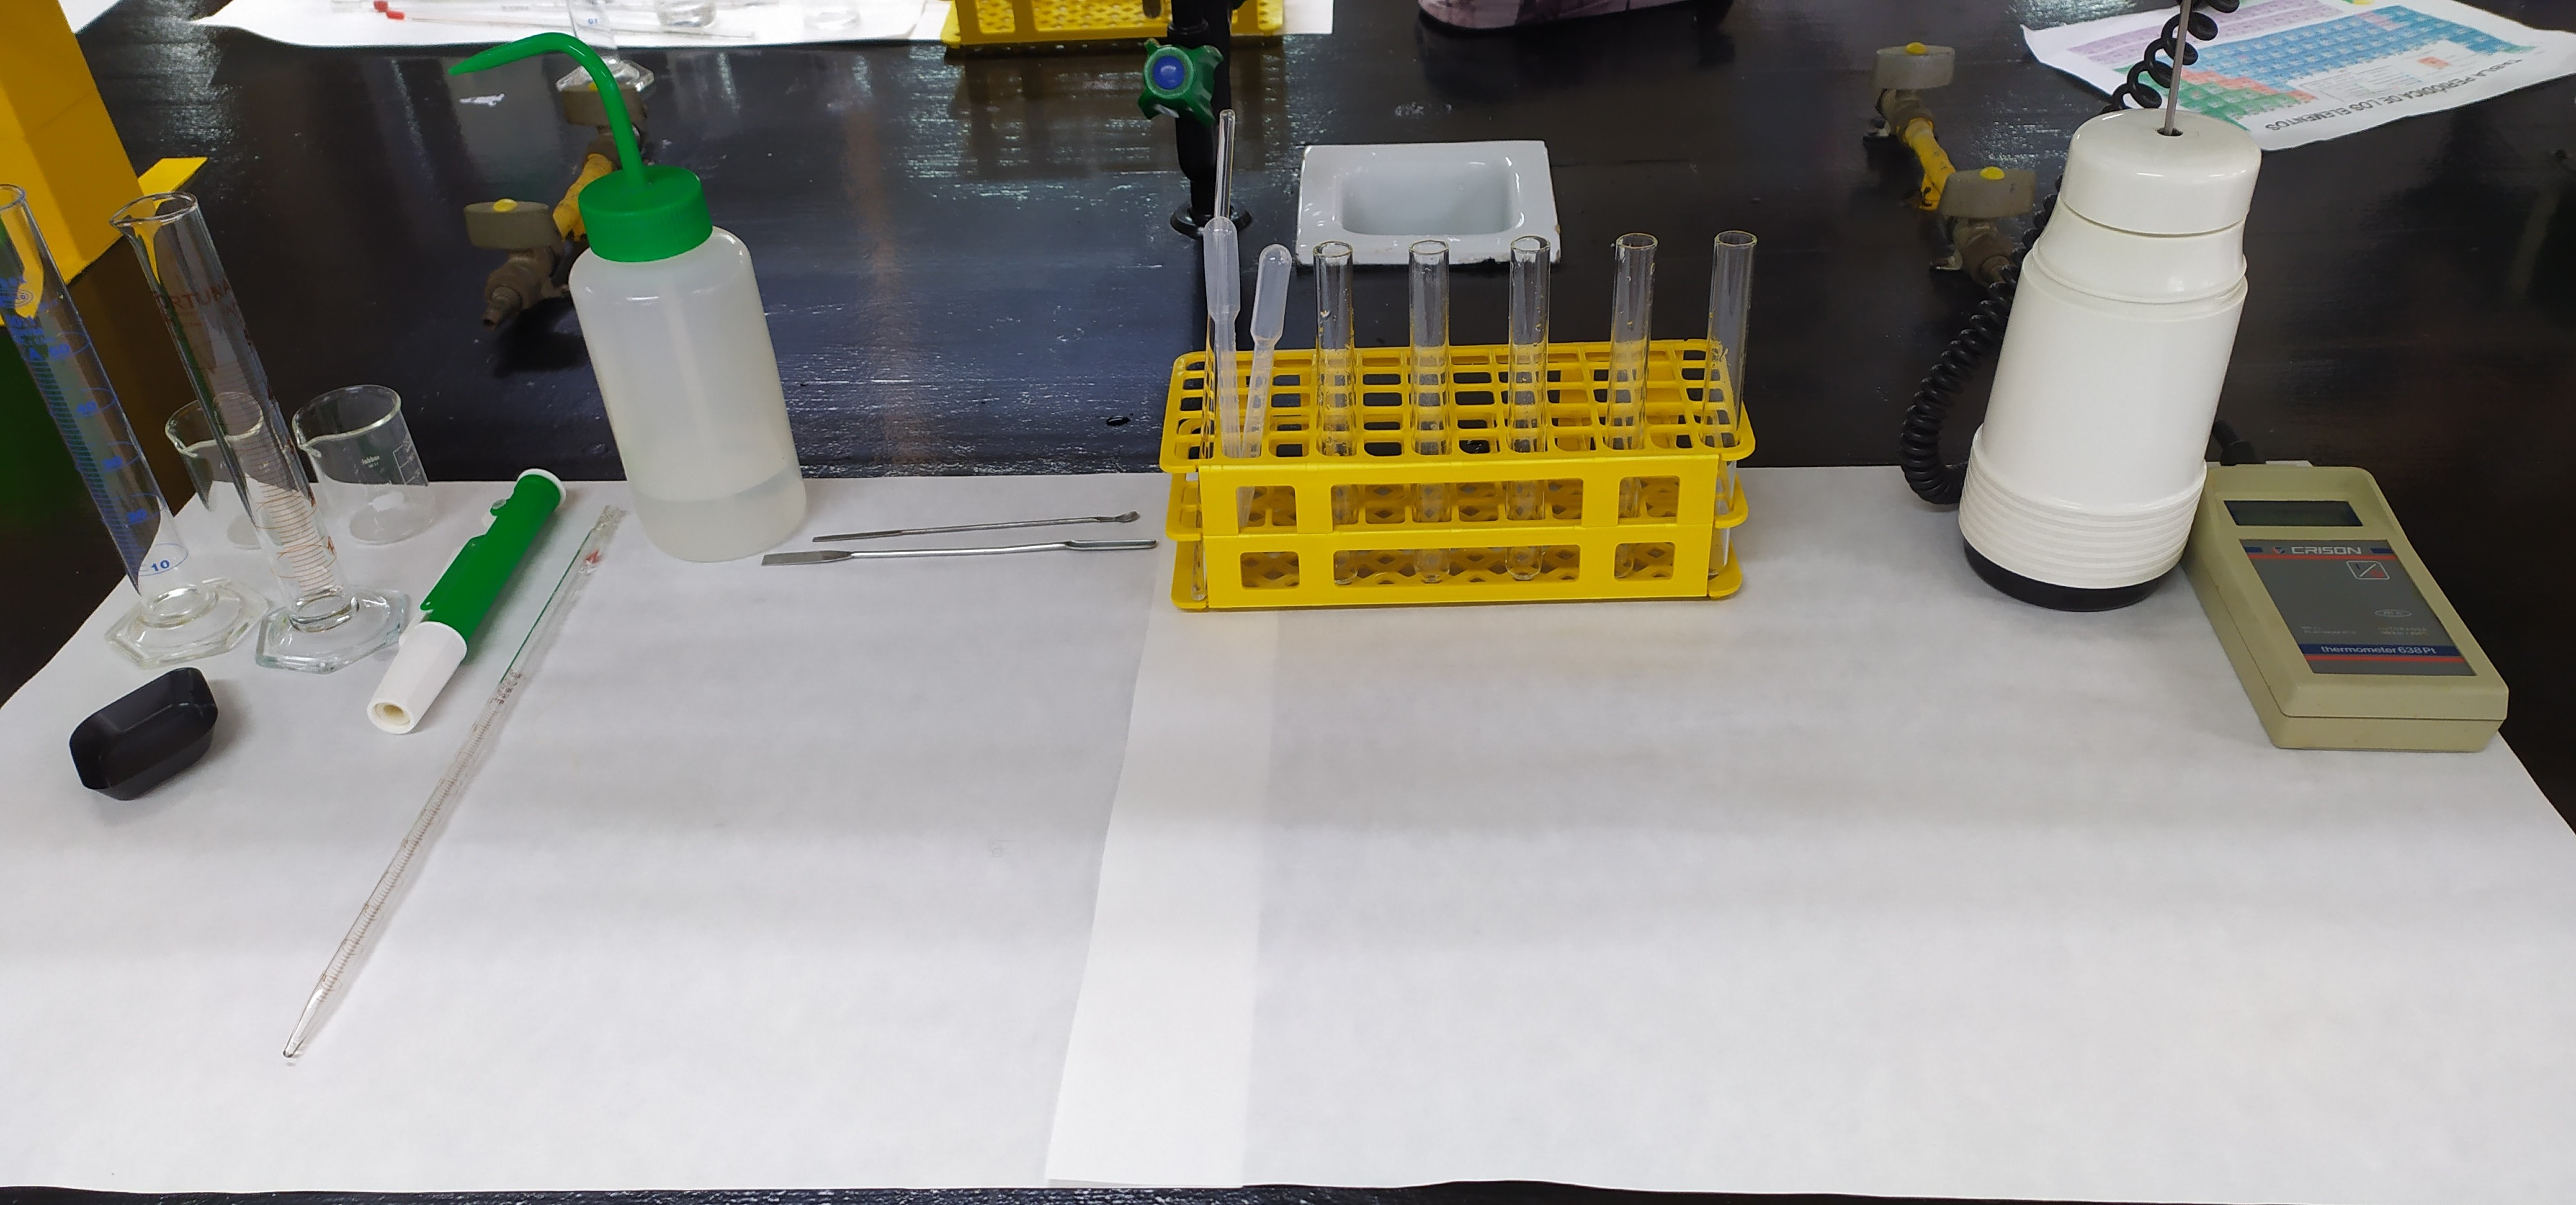
\includegraphics[scale = 0.06]{fotos/mesa2.jpg}
        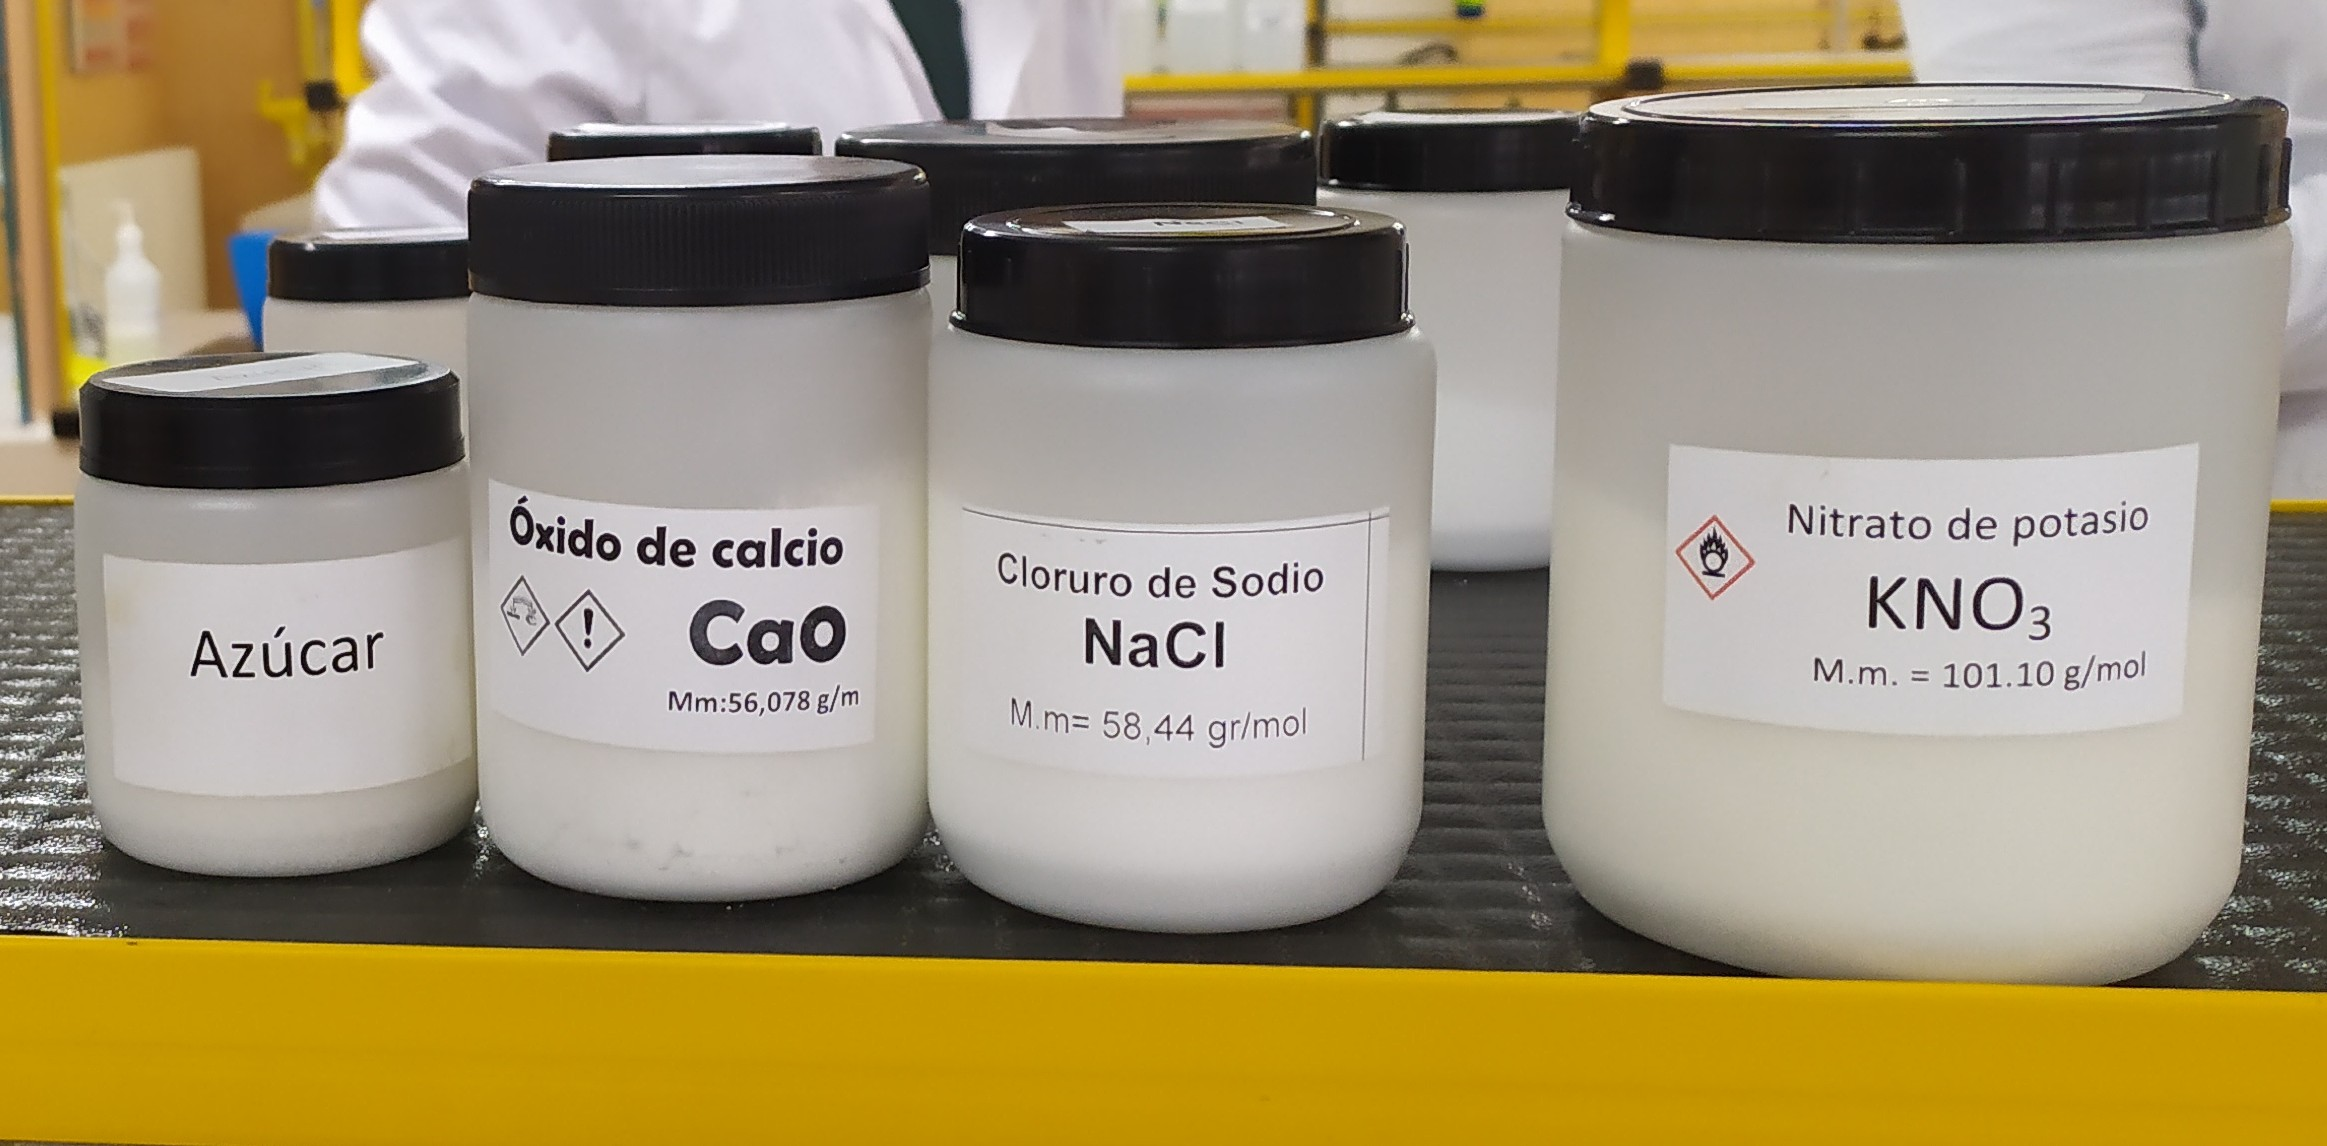
\includegraphics[scale = 0.08]{fotos/soli2.jpg}
    \hspace*{-2.3cm}
    \caption{A la izquierda el material usado y a la derecha los sólidos empleados}
\end{figure}

\clearpage

\section{Procedimiento} 
\noindent En la \textcolor{red}{primera parte} hemos realizado una serie de mezclas de compuestos en tubos de ensayo para determinar los distintos cambios de temperatura. A continuación expongo las distintas mezclas:

\vspace{0.3cm}

i) Mezcla de 0,5 g de óxido de calcio con 3 mL de agua: \newline
\textbf{Proceso exotérmico ($\Delta{T} > 0$)}

\vspace{0.2cm}

ii) Mezcla de un poco de azúcar con unas gotas de ácido sulfúrico concentrado:\newline \textbf{Proceso exotérmico ($\Delta{T} > 0$)}

\vspace{0.2cm}

iii) Mezcla de 0,5 g de nitrato de potasio sólido y 3 mL de agua: \newline
\textbf{Proceso endotérmico ($\Delta{T} < 0$)}

\vspace{0.2cm}

iv) Mezcla de 3 mL
de agua y ácido nítrico concentrado: \newline
\textbf{Proceso exotérmico ($\Delta{T} > 0$)}

\vspace{0.2cm}

v) Mezcla de 0,5 g de cloruro
de sodio y 3 mL de agua: \newline
\textbf{Proceso exotérmico ($\Delta{T} > 0$)}

\vspace{0.3cm}
\noindent Esta parte nos ha servido para tener una primera toma de contacto con lo que vamos a realizar a lo largo de esta práctica. \\

\vspace{0.3cm}

\noindent Ahora vamos a centrarnos en la \textcolor{red}{segunda parte}, en la determinación del equivalente en agua del calorímetro. \\

\noindent En primer lugar, hay que climatizar el calorímetro con agua fría para poder obtener unos resultados próximos a la realidad. Y todos los procesos descritos a continuación tendremos que repetirlos 3 veces para que el resultado sea más preciso. \\

\noindent Tendremos que colocar 50 mL de agua muy fría en el calorímetro agitándolo hasta alcanzar el equilibrio, que en nuestro caso se alcanza a 7.8$^o$C ($T_1$). Una vez alcanzado el equilibrio añadimos 50 mL de agua destilada a temperatura ambiente, previamente medido en una probeta (con una temperatura de 17.5$^o$C, $T_2$), y alcanzamos una temperatura de 12$^o$C ($T_f$) una vez estabilizada la mezcla. 

\clearpage

\noindent Una vez con estos datos podemos determinar el equivalente en agua del calorímetro(W) usando las siguientes fórmulas:

\vspace{0.3cm}

\begin{equation} \label{cedido}
    q_{cedido~ agua~ caliente} = m_{agua~ caliente}\cdot{c_e}\cdot{(T_f - T_2)}
\end{equation}

\begin{equation} \label{ganado}
    q_{\text{ganado~ agua~ fría}} = m_{\text{agua~ fría}}\cdot{c_e}\cdot{(T_f - T_1)}
\end{equation}

\begin{equation} \label{cal}
    q_{\text{calorímetro}} = W\cdot{c_e}\cdot{(T_f - T_1)}
\end{equation}

\begin{equation} \label{sumat}
    q_{cedido~ agua~ caliente} + q_{\text{ganado~ agua~ fría}} + q_{\text{calorímetro}} = 0
\end{equation}

\vspace{0.4cm}

\noindent Para obtener el valor de W sustituimos en la ecuación \eqref{sumat} el valor de las q's definidas en las ecuaciones \eqref{cedido}, \eqref{ganado} y \eqref{cal}. Obtenemos así esta ecuación, de la que podemos cancelas las $c_e$:

\[ m_{agua~ caliente}\cdot{c_e}\cdot{(T_f - T_2)} + m_{\text{agua~ fría}}\cdot{c_e}\cdot{(T_f - T_1)} + W\cdot{c_e}\cdot{(T_f - T_1)} = 0\]

\noindent Despejamos la W y se nos queda esta ecuación:

\[ W = \frac{-m_{agua~ caliente}\cdot{(T_f - T_2)} - m_{\text{agua~ fría}}\cdot{(T_f - T_1)}}{T_f - T_1)}\]

\vspace{1cm}

\begin{table}[h]
    \centering
\begin{tabular}{ | c | c | c | c |} 
    \hline
    \multicolumn{4}{ |c| }{Resultados} \\
    \hline
    $T_1$ $(^oC)$ & 7.8 & 5.5 & 4.2 \\  
    $T_2$ $(^oC)$ & 15 & 17.5 & 17.5  \\
    $T_f$ $(^oC)$ & 12 & 11.1 & 10.1 \\
    \hline
    W (J)  & 15.48 & 7.14 & 12.71 \\  

    \hline
\end{tabular}
    \caption{Tabla de los datos obtenidos  tras las mediciones y cálculos}
    \label{tabla-temp y w}
\end{table}

\vspace{0.4cm}

\noindent A continuación abordaremos el \textcolor{red}{tercer punto} de esta práctica, que es la determinación de la entalpía de neutralizar un ácido fuerte con una base fuerte.\\


\noindent Para hacer esto, medimos en una probeta 50 mL de  disolución 2 M de hidróxido de sodio (NaOH) y lo colocamos en el calorímetro. A continuación, introducimos otros 50 mL de ácido clorhídrico 2M (HCl). Ambas disoluciones por separado están a temperatura ambiente (unos 16$^o$C) y tras reaccionar en el calorímetro obtenemos una temperatura resultante de 28.7$^o$C.\\


\noindent Una vez que sabemos la temperatura de reacción, la entalpía de reacción la podemos sacar de la fórmula \eqref{entalps}, teniendo los valores siguientes: $c_e$ = 4.18, $m_{mezcla}$ = 100 g, W = 11.78 J (la media de todos los trabajos obtenidos previamente) y $\Delta{T}$ = 28.7 - 16 = 12.7$^o$C (temperatura de reacción menos la ambiente en la primera medida). Por lo tanto, de la ecuación \eqref{entalps} podemos despejar la entalpía de reacción ($\Delta{H_{reaccion}}$ fácilmente y se pueden sustituir los valores par obtener dicho valor. Pero puesto que en esta parte realizamos también 3 medidas para obtener una mayor precisión, voy a hacer una tabla para que se vean mejor los datos y los resultados obtenidos.

\vspace{0.4cm}

\begin{equation} \label{entalps}
    \Delta{H_{reaccion}} + m_{mezcla}\cdot{c_e}\cdot{\Delta{T}} + W\cdot{c_e}\cdot{\Delta{T}} = 0
\end{equation}

\vspace{0.4cm}

\begin{table}[H]
    \centering
\begin{tabular}{ | c | c | c | c |} 
    \hline
    \multicolumn{4}{ |c| }{Resultados} \\
    \hline
    $T_r$ $(^oC)$ & 28.7 & 30.3 & 29.8 \\  
    $\Delta{T}$ $(^oC)$ & 12.7 & 14.3 & 13.8  \\
    \hline
    $\Delta{H_r}$ $(J)$ & -5933.95 & -6681.54 & -6447.92 \\   

    \hline
\end{tabular}
    \caption{Tabla de las entalpías obtenidas}
    \label{entalp}
\end{table}


\noindent Finalmente, nos encontramos ya en la \textcolor{red}{última parte} de la práctica, que es bastante parecida al apartado anterior pero en el ácido fuerte lo cambiamos por un ácido débil. \\

\noindent Ahora, mediremos 50 mL de hidróxido sódico 2M y lo añadimos en el calorímetro, para a continuación repetir el mismo proceso con 50 mL de ácido acético 2M ($CH_3COOH$) . En esta parte usaremos también la ecuación \eqref{entalps}. Y haremos otra tabla para ver los datos de las 3 mediciones realizadas.

\begin{table}[H]
    \centering
\begin{tabular}{ | c | c | c | c |} 
    \hline
    \multicolumn{4}{ |c| }{Resultados} \\
    \hline
    $T_r$ $(^oC)$ & 28.3 & 28 & 28.1 \\  
    $\Delta{T}$ $(^oC)$ & 12.3 & 12 & 12.1  \\
    \hline
    $\Delta{H_r}$ $(J)$ & -5748.09 & -5607.89 & -5654.62 \\   

    \hline
\end{tabular}
    \caption{Tabla de las entalpías obtenidas}
    \label{entalp-2}
\end{table}

\clearpage

\section{Cuestiones}

\noindent\textcolor{BlueViolet}{\textbf{\textit{a) Escriba las reacciones correspondientes a los procesos estudiados en el primer apartado, indicando si son endotérmicos o exotérmicos.}}}\\


    \vspace{0.1cm}
    
     Este apartado ya lo he completado parcialmente en el procedimiento, lo único que falta es poner la correspondiente reacción:\\
    
    \vspace{0.2cm}
    
    i)$~ CaO(g) + H_2O(l) ~\rightleftharpoons ~Ca(OH)_2$
    
    \vspace{0.2cm}
    
    ii)$~ C_{12}H_{22}O_{11}(s) + H_2O(l) ~\rightleftharpoons ~ H_2O(g) + C(s)$
    
    \vspace{0.2cm}
    
    iii)$~ H_2O(l) + KNO_3(s) ~\rightleftharpoons ~ HNO_3 + KOH$
    
    \vspace{0.2cm}
    
    iv)$~ HNO_3(l) + H_2O(l) ~\rightleftharpoons ~ NO_3^- + H_3O^+$
    
    \vspace{0.2cm}
    
    v)$~ NaCl(s) + H_2O(l) ~\rightleftharpoons ~ NaOH + HCl$\\
    
    \vspace{0.3cm}

\noindent\textcolor{BlueViolet}{\textbf{\textit{b) Determine los valores de la entalpía de neutralización de las dos reacciones
estudiadas.}}}\\

    \vspace{0.2cm}
    
    Las entalpías obtenidas podemos observarlas en los cuadros \ref{entalp} y \ref{entalp-2}\\
    
    \vspace{0.4cm}

\noindent\textcolor{BlueViolet}{\textbf{\textit{c) Calcule teóricamente la entalpía de la reacción de neutralización y compare el
resultado teórico con los resultados experimentales obtenidos.}}}\\

 Calculemos la entalpía de reacción teóricamente para ver si nuestros datos experimentales son correctos:\\
\[\Delta{H_{r}} = \Delta{H_{f}(H_2O)} - \Delta{H_{f}(H^+)} - \Delta{H_{f}(OH^-)} = -285.8 - 0 - (-230) = -55 kJ\]

 Podemos observar que los valores experimentales obtenidos a lo largo de la práctica se aproximan bastante al teórico calculado.















% PRÁCTICA 3
\chapter[Práctica 3]{3. Ph y disoluciones reguladoras}
\thispagestyle{empty}
\vspace{1cm}
\begin{figure}[h]
    \centering
    \hspace*{-0.2cm}
    \includegraphics[width=1\textwidth]{prac3/portada.jpg}
    \hspace*{-0.4cm}
\end{figure}
\section{Introducción}
\noindent El objetivo de esta práctica es el estudio del comportamiento de diferentes disoluciones amortiguadoras (también llamadas disolución tampón) mediante varias medidas del pH. También se realizará una valoración potenciométrica (es decir, basada en la diferencia de potencial a través de un electrodo) con \ce{H3PO4}.
\section{Inventario}
\vspace{0.4cm}
Para esta práctica hemos usado:

\begin{multicols}{2}
    \begin{itemize}
        \item 1 Peachímetro
        \item 2 Pipetas graduadas
        \item 3 Propipetas
        \item 1 Colador
        \item 1 Varilla metálica
        \item 1 Placa de calor
        \item 2 Frascos lavadores
        \item 4 Vasos de precipitados
        \item 1 Embudo
        \item 3 Erlenmeyer
        \item 2 Espátulas
        \item 2 Probetas
        \item Líquidos: 
        \item Naranja de metilo ($\ce{C14H14N3NaO3S}$)
        \item Fenolftaleína ($\ce{C20H14O4}$)
        \item Agua ($\ce{H2O}$)
    \end{itemize}
\end{multicols}

\vspace{0.3cm}
Podemos ver parte de lo nombrado anteriormente en la siguiente fotografía:

\begin{figure}[H]
    \centering
    \hspace*{-2.3cm}
        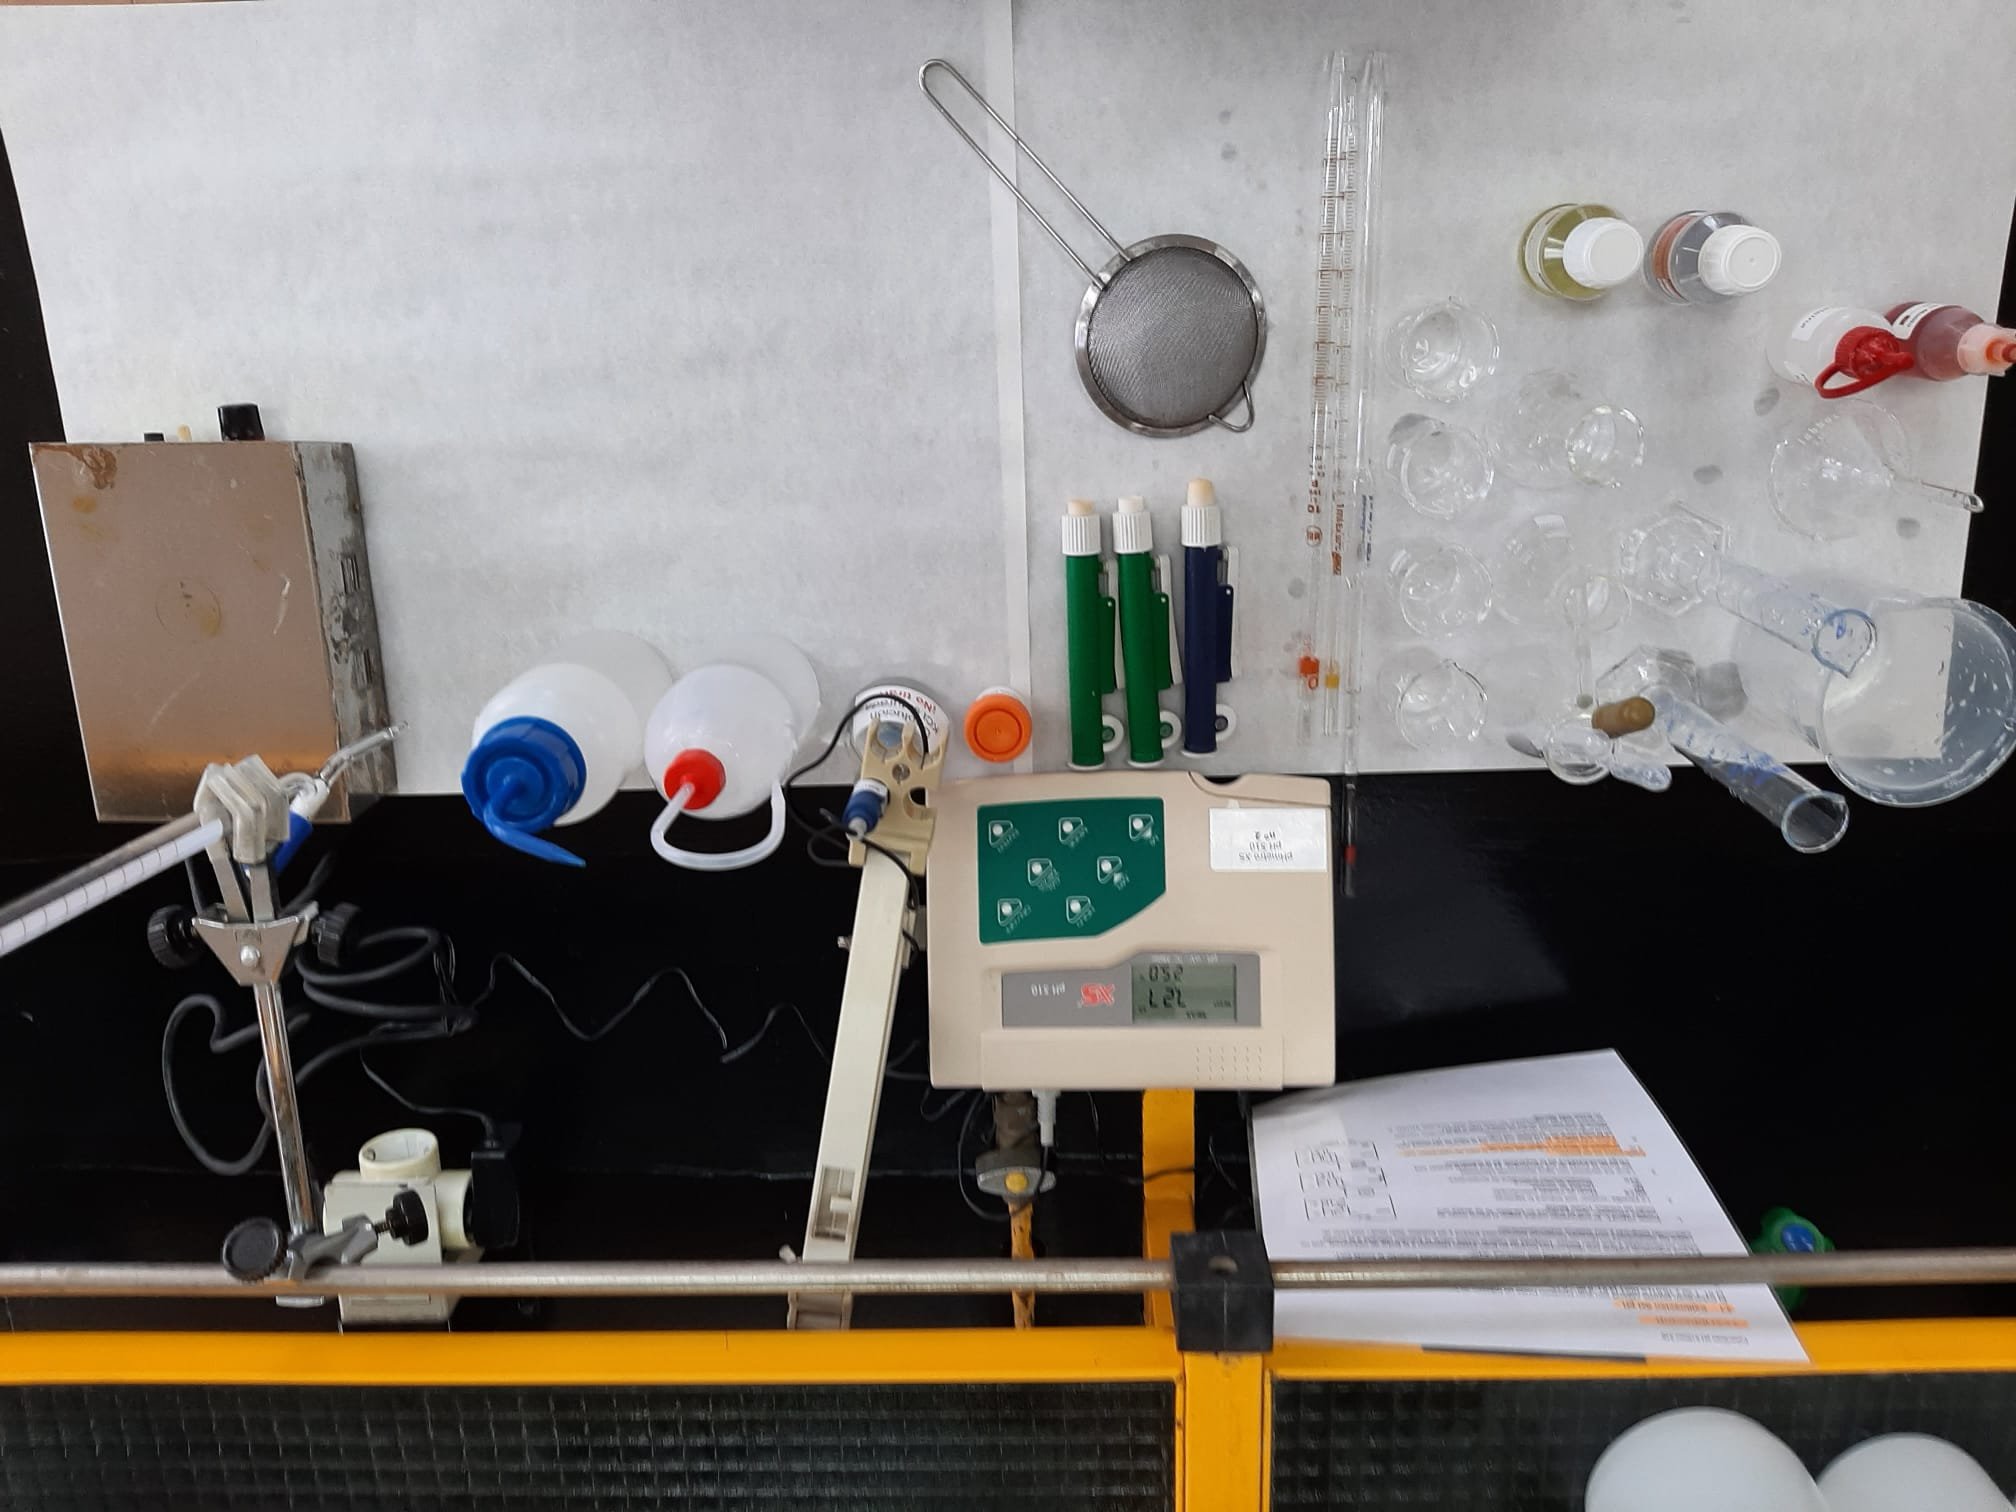
\includegraphics[scale = 0.15, angle=180]{prac3/Inventario3.jpeg}
    \hspace*{-2.3cm}
    \vspace{-2cm}
\end{figure}

\clearpage

\section{Procedimiento}
\noindent En primer lugar, mediremos el pH de ciertas disoluciones amortiguadoras, de la cual siempre tendremos $V_{disolución} = 30 \si{ml}$ a los cuales añadiremos $10 \si{ml}$ primero de una base fuerte (\ce{NaOH} 1\si{M}) y luego de un ácido fuerte (\ce{HCl} 1\si{M}). Posteriormente, repetiremos la adición de esta base y este ácido, ahora añadiéndolos a 30 \si{ml} de agua destilada.\\\\
Para la valoración potenciométrica, añadiremos unas gotas de naranja de metilo y de fenolftaleína a 10 \si{ml} de \ce{H3PO4}. Ahora, añadiremos \ce{NaOH} hasta que se vuelva amarillo desde su color rosa inicial para luego seguir añadiendo hasta que vuelva a dicho rosa. Esta experiencia la repetiremos tres veces para poder comparar las medidas de volumen obtenidas.\\\\
Finalmente, repetiremos el paso anterior pero ahora de forma mucho más precisa: con ayuda de la varilla imantada y del pH-metro, añadiremos \ce{NaOH} de 2 \si{ml} en 2 \si{ml}, excepto cerca del volumen de viraje, donde añadimos de 0,2 en 0,2 \si{ml}, e iremos midiendo los cambios de pH en estos intervalos.

\clearpage
\section{Cuestiones}
\noindent\textcolor{BlueViolet}{\textbf{\textit{a) Busque en el Handbook el valor de $K_a$ para el ácido acético.}}}\\\\
\noindent El valor de $K_a$ que encontramos en el \textquote{\textit{CRC Handbook of Chemistry and Physics}} es de $K_a = 1.75\cdot 10^{-5}$ a $25^{\circ} C$\\\\
\noindent\textcolor{BlueViolet}{\textbf{\textit{b) Comente si:
    \begin{itemize}
        \item El $pH$ de la disolución tampón es función de la concentración.
        \item La capacidad amortiguadora depende de la concentración de la disolución tampón.
        \item Coinciden los valores de $pH$ esperados teóricamente con los medidos experimentalmente. Comente las posibles fuentes de error.
    \end{itemize}
}}}

\noindent Para esta primera parte de la cuestión podemos afirmar que el pH de cualquier disolución tampón es proporcional directamente a su concentración. En concreto a la relación entre la concentración de sal y de ácido que nos dice la ecuación de Henderson-Hasselbalch:
\[pH = pK_a + \log\left(\frac{[S]}{[A]}\right)\]
\noindent En segundo lugar, estudiaremos si la capacidad amortiguadora de la disolución tampón depende también de la concentración. Y efectivamente, lo hace, puesto que depende no solo de la concentración de la disolución, sino de la concentración de todo el sistema, aumentando junto con ella, alcanzando el máximo cuando el cociente se aproxima a 1.\\\\
\noindent Por último, comprobaremos si los valores del ph experimentales coinciden con los esperados teóricamente. Para el caso de viraje de rosado a amarillo, de forma teórica vemos que deberíamos notar el cambio alrededor de los $11 ± 0.5 \si{ml}$, pero experimentalmente la notamos en $10.4 ± 0.2 \si{ml}$. De igual manera ocurre en el cambio de vuelta de amarillo a rosa. Debería cambiar sobre de los $22 ± 0.5 \si{ml}$ pero lo hace entorno a los $21.4 ± 0.2 \si{ml}$.\\\\
\noindent La mayor parte de este error se debe claramente al factor humano. Nuestra primera valoración es potenciométrica, tratamos de dilucidar en qué instante la disolución lleva a cabo este viraje de color, pero introducimos una gran cantidad de error al no ser un punto claro el que produce este viraje.
\clearpage

\noindent Vamos a representar en una gráfica la tabla de ph frente al volumen de \ce{NaOH} añadido. La tabla que describe los datos está representada en la hoja 21.

\begin{figure}[H]
    \centering
    \hspace*{-2.3cm}
        \includegraphics[scale = 1]{prac3/Gráfica3).jpg}
    \hspace*{-2.3cm}
    \caption{Ph frente al volumen añadido}
\end{figure}

\noindent Se puede observar en la gráfica un ajuste polinomial de grado 6 que aproxima nuestros datos. Se aprecian a la perfección los dos cambios del pH, así como el ascenso final que se sale de nuestros datos.\\\\
\noindent A continuación, representaremos la curva derivada de esta mediante el cociente incremental para poder ver más claramente cuales son nuestros puntos de viraje. Para ello, añadimos a nuestra tabla de datos de ph y volúmen, los apartados que se basan en las siguientes expresiones:

\[\frac{V_{i+1}+V_i}{2}\]
\[\frac{pH_{i+1}-pH_i}{V_{i+1}-V_i}\]
\clearpage

\begin{figure}[H]
    \centering
    \hspace*{-2.3cm}
        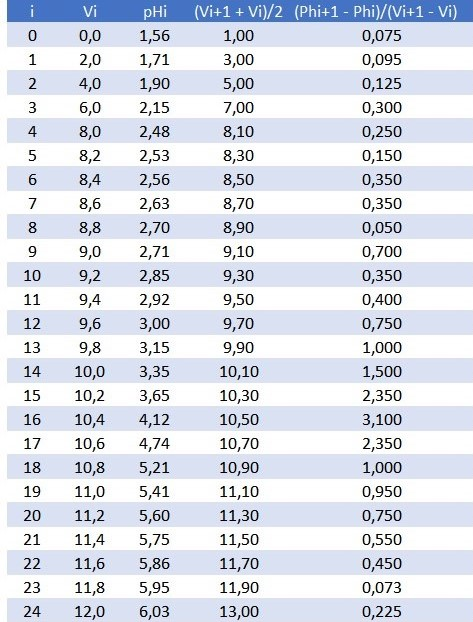
\includegraphics[scale = 0.75]{prac3/tabla31.jpg}
        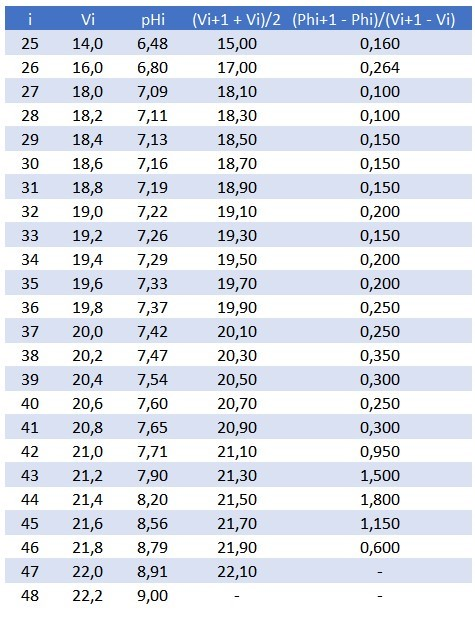
\includegraphics[scale = 0.75]{prac3/tabla32.jpg}
    \hspace*{-2.3cm}
\end{figure}

\noindent Una vez obtenidos los datos, representamos gráficamente la derivada de la gráfica anterior, que resulta muy interesante por la aparición de dos picos explícitos allá donde el pH ha variado muy velozmente.

\begin{figure}[H]
    \centering
    \hspace*{-2.3cm}
        \includegraphics[scale = 0.8]{prac3/Gráfica3.1.jpg}
    \hspace*{-2.3cm}
\end{figure}
\clearpage

\noindent En esta gráfica, podemos observar que los máximos se encuentran en los puntos 10.4 y 22.5 siendo el primero más pronunciado que el segundo. Estos valores coinciden con lo observado experimentalmente.\\\\
\noindent Por último, calcularemos la concentración inicial de ácido fosfórico - \ce{H3PO4} – a partir de estos volúmenes. Si sabemos los volúmenes de viraje, podemos plantear la ecuación que rige esta reacción para ver la relación molar entre \ce{H3PO4} y \ce{NaOH}. Como sabemos la concentración de la disolución de \ce{NaOH}, podremos calcular los moles de \ce{H3PO4}, y con ellos el valor pedido.\\\\
\noindent La reacción se desarrolla de la siguiente forma:
\[\ce{H3PO4 + NaOH -> H2PO2^- + Na^+ + H2O}\]
Con la reacción ajustada, comprobamos que a cada mol de \ce{NaOH} le corresponde un mol de ácido fosfórico. Haremos entonces el siguiente cambio de conversión para obtener los moles de ácido, tomando como volumen de \ce{NaOH} el primer volumen de viraje:
\[10.3\si{ml}\ \text{de}\ \ce{NaOH}\cdot\frac{1\si{L}}{1000\si{ml}}\cdot \frac{1\si{mol}\ \ce{NaOH}}{1\si{L}\ \text{disolución}\ \ce{NaOH}}\cdot\frac{1\si{mol}\ \ce{H3PO4}}{1\si{mol}\ \ce{NaOH}} = 0.0103\si{mol}\ \ce{H3PO4}\]
Ahora obtenemos la molaridad:
\[M_{\ce{H3PO4}} = \frac{n_{\ce{H3PO4}}}{L_{\ce{H3PO4}}} = \frac{0.0103}{0.01} = 1.03\si{M}\]
\noindent Probablemente gran parte del error se debe a la búsqueda de colores más intensos de lo debido a la hora de realizar la valoración potenciométrica. Esto ha hecho que la disolución avance más de lo debido en la valoración, haciendo que su pH aumente excesivamente antes de tomar los volúmenes de \ce{NaOH} que supusimos serían de viraje.\\\\
\noindent En lo respectivo a las gráficas realizadas en la tercera cuestión, ambas representan de forma muy fidedigna los cambios de pH sufridos por la disolución. En la primera, podemos ver de forma directa el crecimiento del pH conforme aumentamos el volumen de la base. 
\noindent Mientras estemos alejados de los puntos de viraje, destacamos como el crecimiento es muy cercano a un crecimiento lineal. Sin embargo, en estos puntos críticos nombrados, el crecimiento se vuelve prácticamente exponencial.\\\\
\noindent Esto queda reflejado muy claramente en la segunda gráfica, la de la derivada, que mantiene valores constantes hasta llegar a máximos muy pronunciados, en especial el primero, que muestran estos puntos de viraje muy bruscos. Concluimos que ambas gráficas concuerdan con los resultados experimentales y teóricos, en el sentido de representar cambios bruscos en el color de la disolución.

% PRÁCTICA 4
\chapter[Práctica 4]{4. Determinación de la dureza del agua}
\thispagestyle{empty}
\vspace{1cm}
\begin{figure}[h]
    \centering
    \hspace*{-0.2cm}
    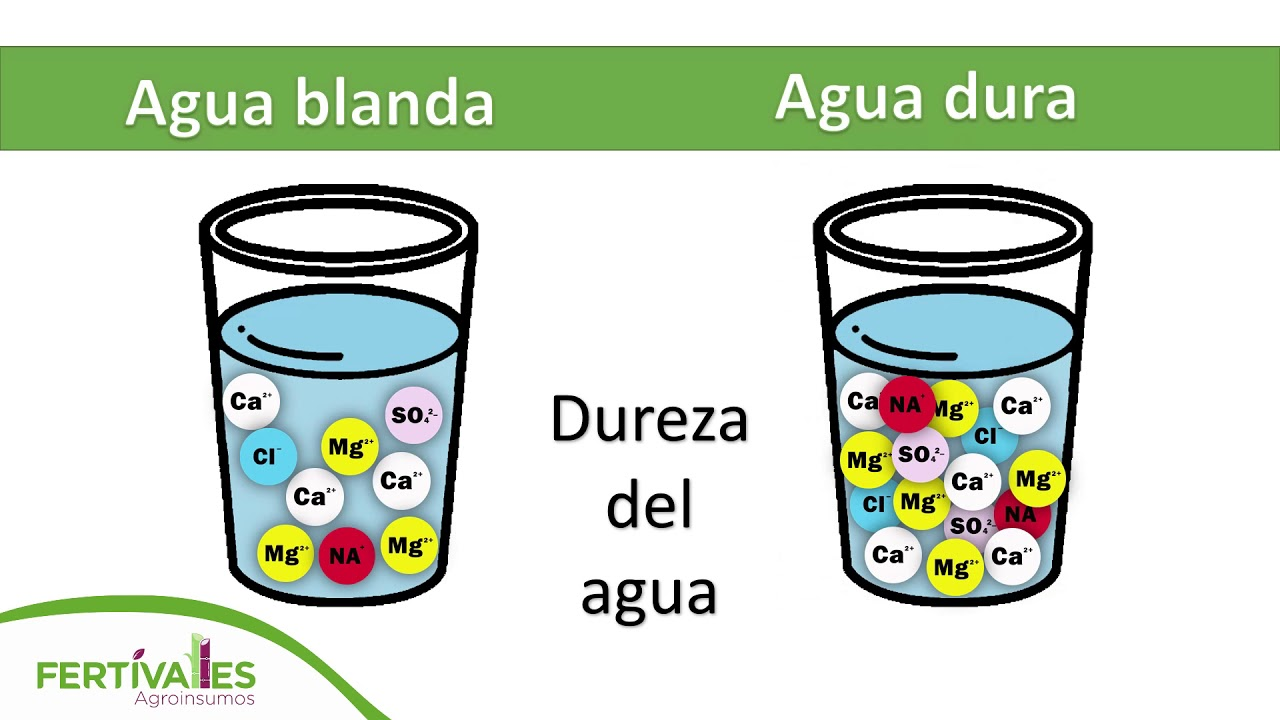
\includegraphics[width=1\textwidth]{fotos/dureza.jpg}
    \hspace*{-0.4cm}
\end{figure}
\section{Introducción}   %revisaaaaaaaaaaaaaarrrrrrr
\noindent La finalidad de esta práctica es obtener la dureza del agua mediante una serie de reacciones donde el primer proceso nos dará el volumen de calcio y magnesio presente en el agua (del grifo) y el segundo proceso nos dará sólo el volumen del magnesio, que nos permitirá calcular la cantidad de calcio presente en el agua, para así poder volver a la primera parte y calcular la cantidad de magnesio. Con estas dos magnitudes seremos capaces de calcular lo que nos pide la práctica: la dureza del agua. A lo largo de esta práctica nos va a ser útil conocer qué significan los distintos colores que vamos a obtener:

\begin{multicols}{3}
    $pH < 7$ ~$\rightsquigarrow$ ~ rojo vino
    
    \vspace{0.1cm}
    
    $7 < pH < 11.5$ ~$\rightsquigarrow$ ~ azul
    
    \vspace{0.1cm}
    
    $pH > 11.5$ ~$\rightsquigarrow$ ~ naranja
\end{multicols}

\section{Inventario}  
\noindent En esta práctica contamos con:
\begin{multicols}{2}
    \begin{itemize}
        \item 2 erlenmeyer
        \item 3 vasos de precipitados
        \item Un embudo Büchner
        \item Un matraz kitasatos
        \item Un embudo
        \item Una varilla
        \item Una espátula
        \item Una pipeta 
        \item Una bureta
        \item Una placa calefactora
        \item Unos guantes de silicona
        \item Amoniaco ($NH_3$)
        \item Indicadores: Rojo de metilo y Negro de eriocrom T
        \item Oxalato de sodio ($C_2Na_2O_4$)
        \item Ácido clorhídrico (HCl)
    \end{itemize}
\end{multicols}

\begin{figure}[H]
    \centering
    \hspace*{-3cm}
        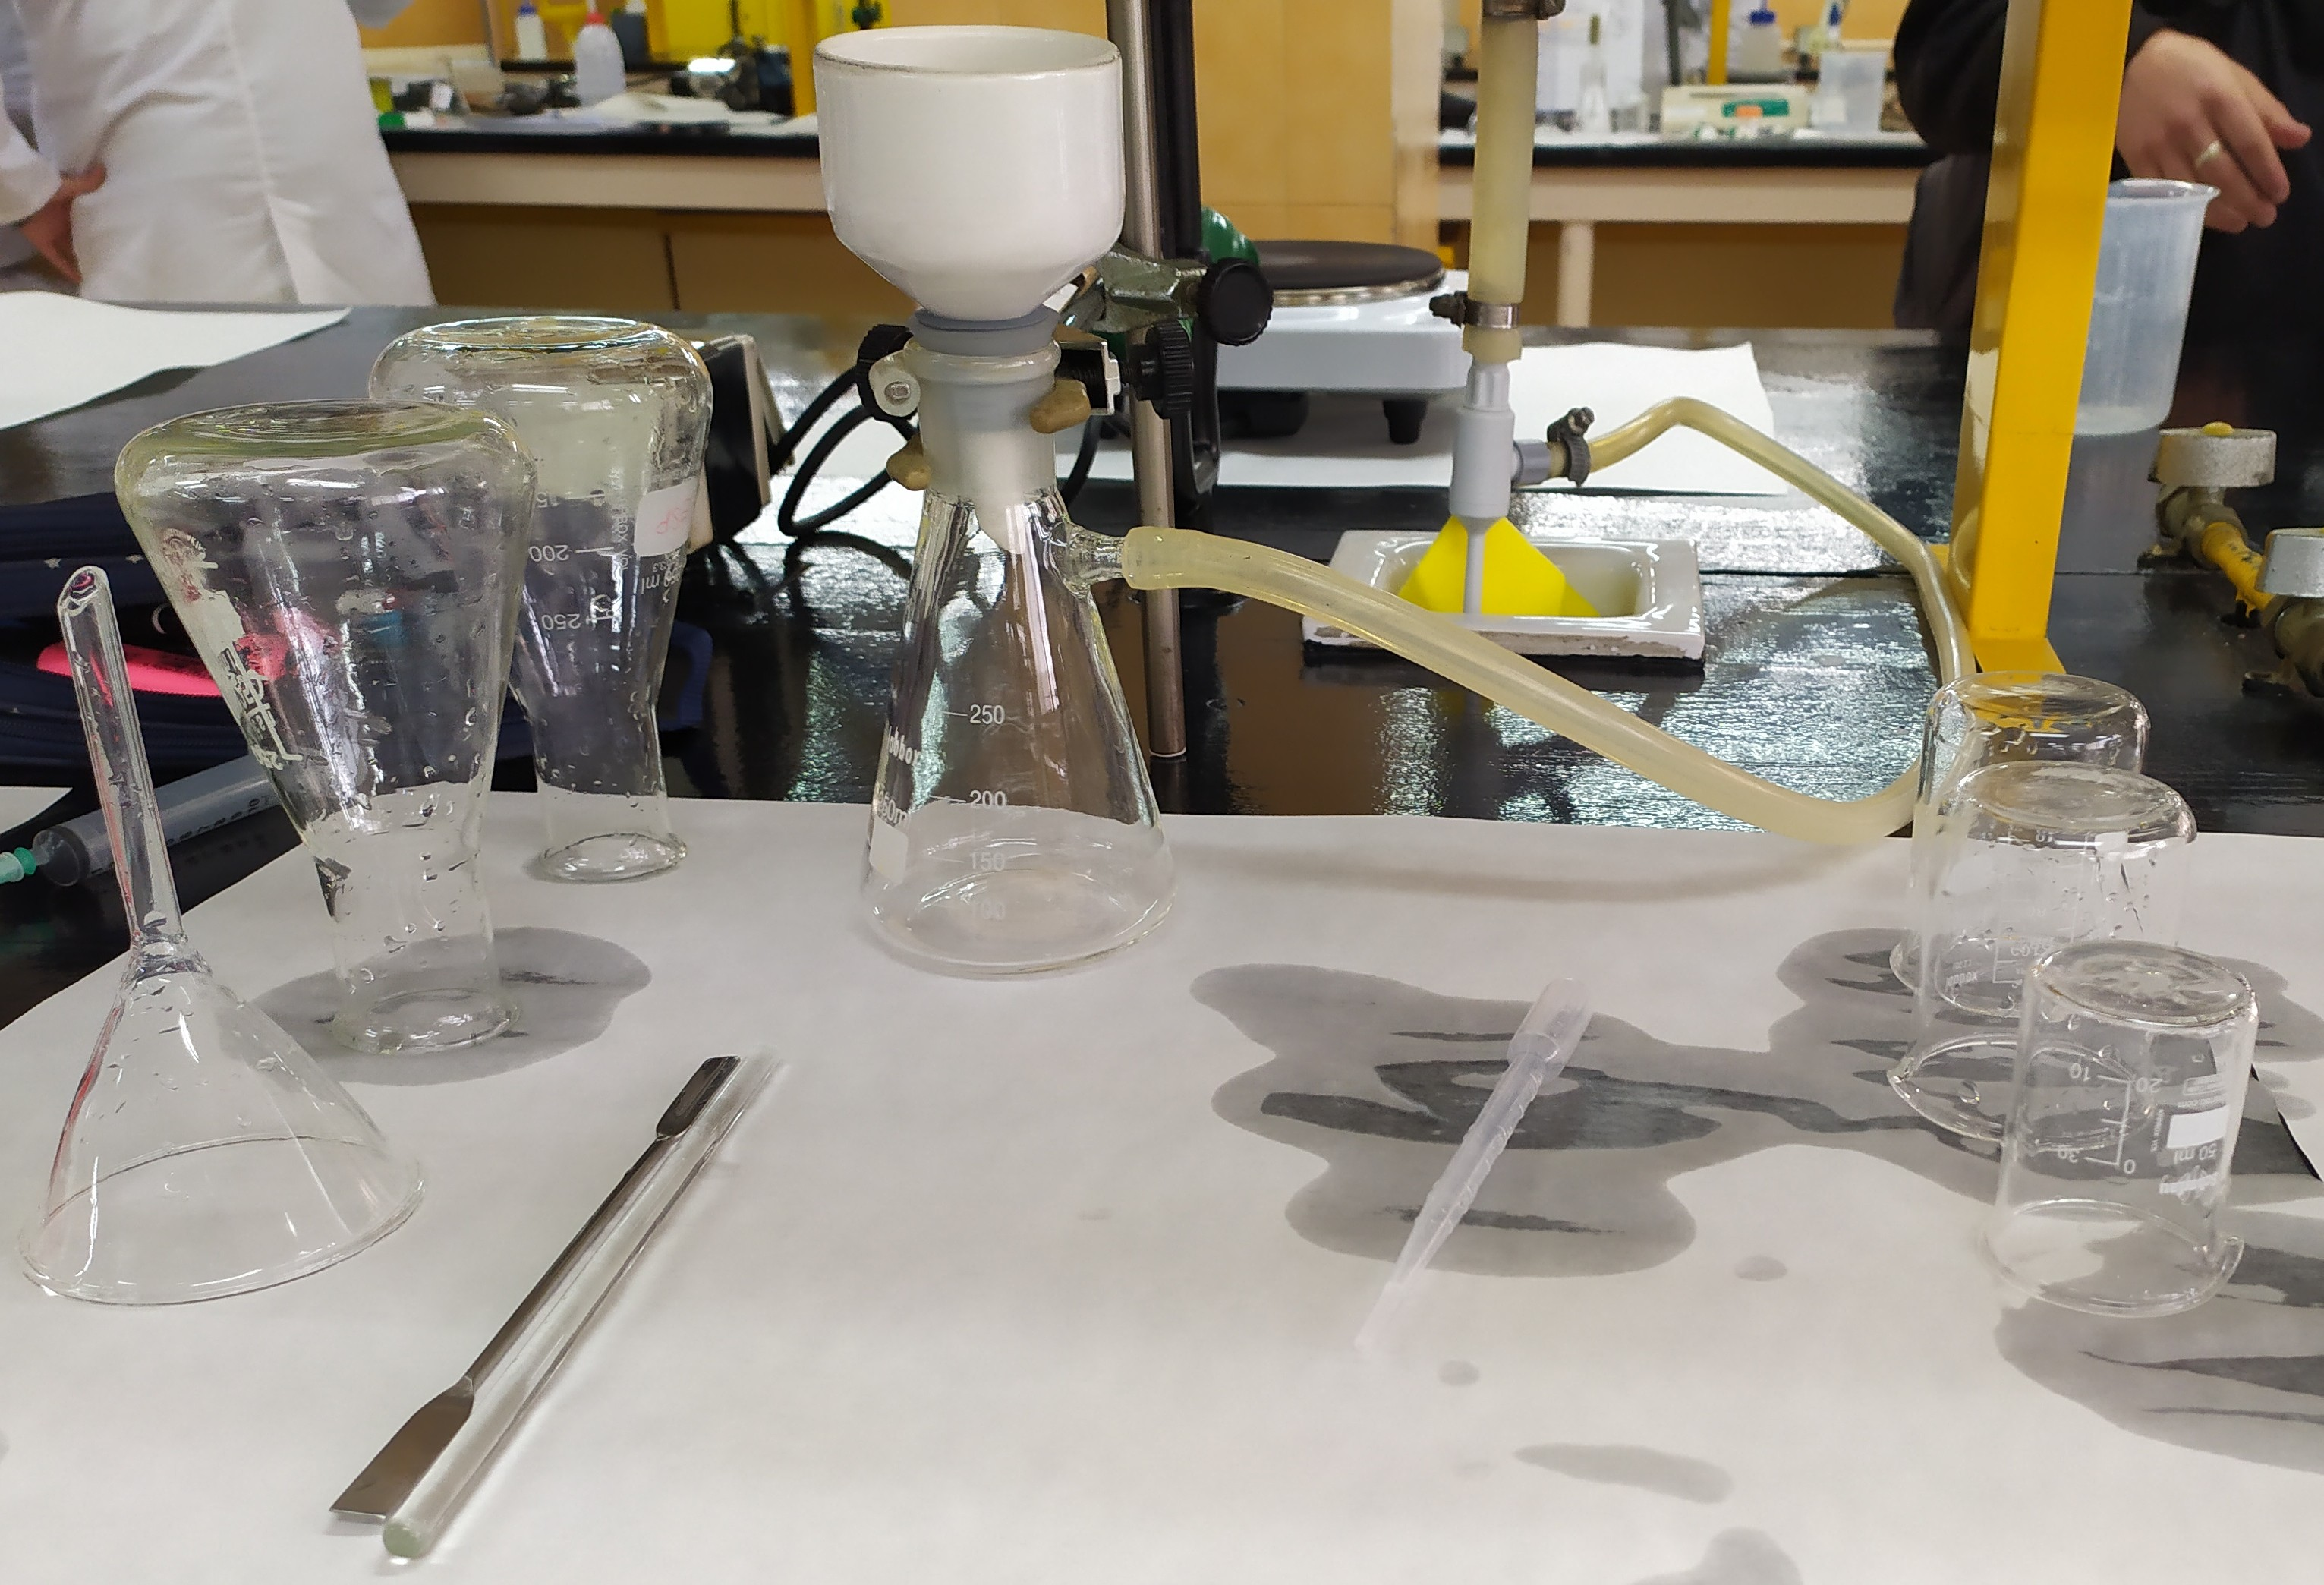
\includegraphics[scale = 0.049]{fotos/set4.jpg}
        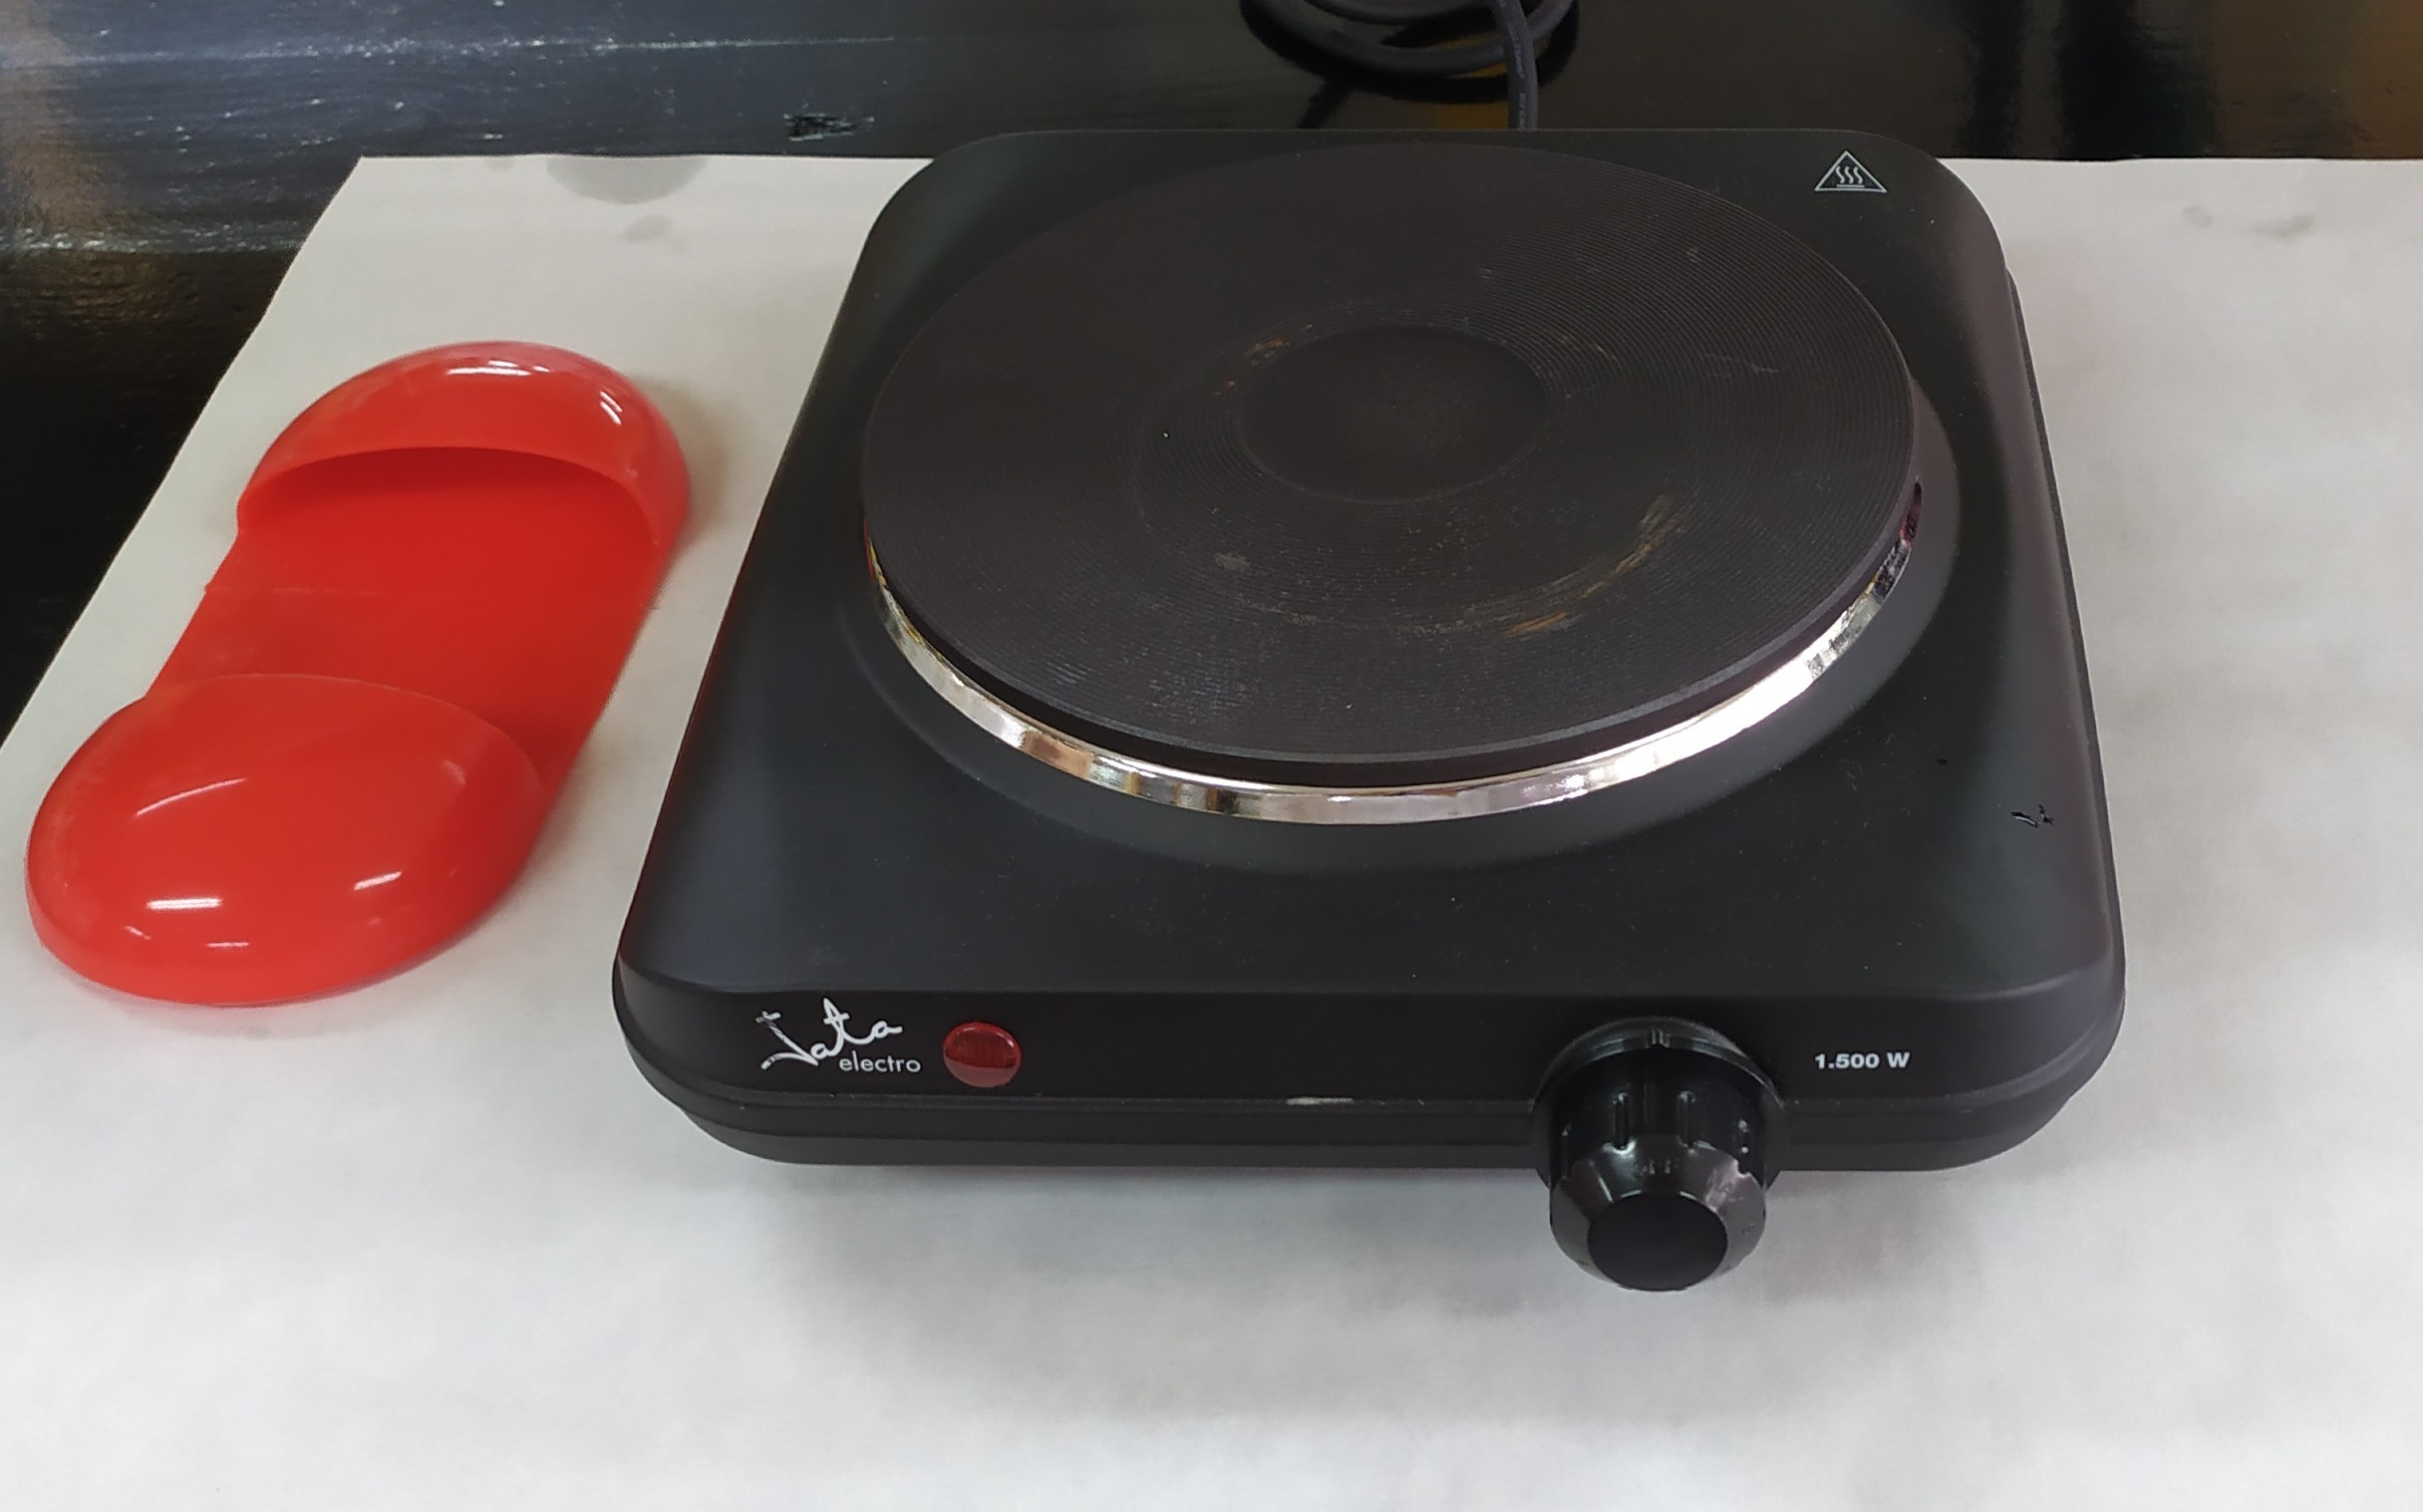
\includegraphics[scale = 0.0673]{fotos/placa4.jpg}
        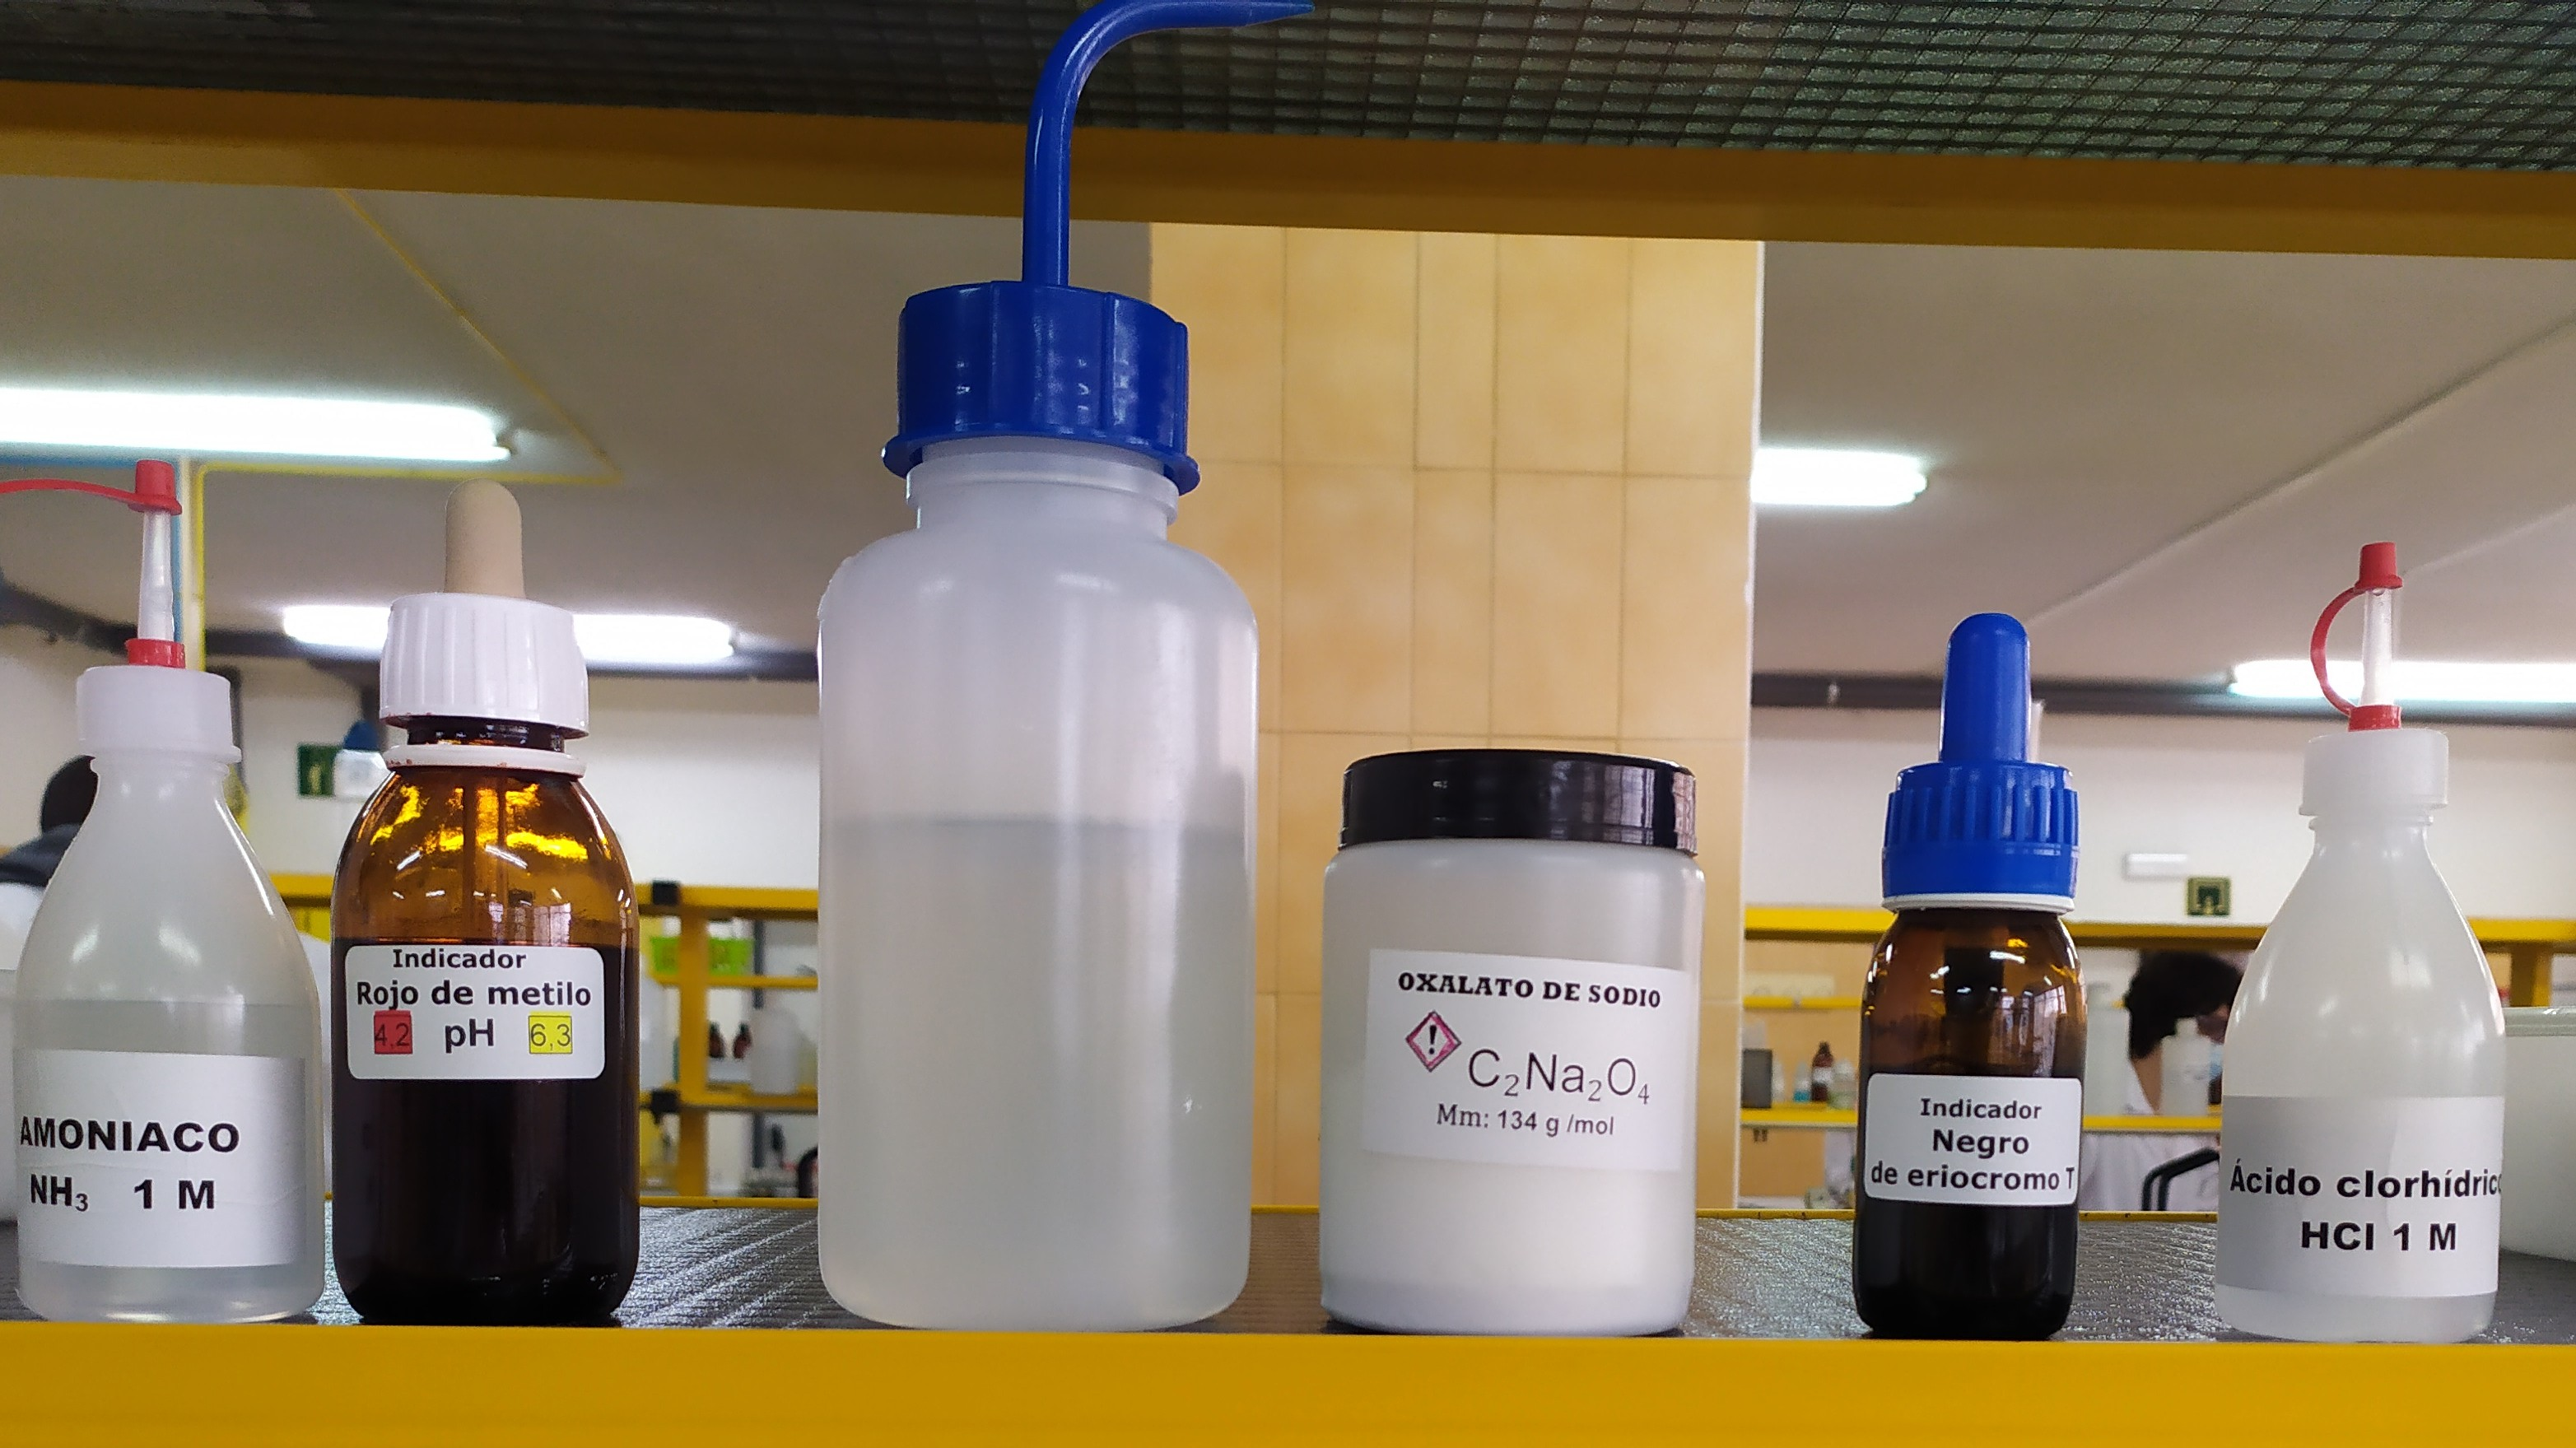
\includegraphics[scale = 0.058]{fotos/liqui4.jpg}
    \hspace*{-3cm}
    \caption{Material descrito}
\end{figure}
\vspace{-3cm}
\clearpage

\section{Procedimiento}
\noindent Esta práctica consta de dos partes, en la primera determinamos la dureza total del agua, y en la segunda la dureza específica magnésica y cálcica. Y para determinar dicha dureza usaremos el agua del grifo.

\vspace{0.2cm}

\noindent En la \textcolor{red}{primera parte} mediremos con un matraz aforado $100 mL$ de agua, lo pasamos a un erlenmeyer donde añadimos unas 10 gotas de rojo metilo hasta obtener un color amarillo y luego acidificamos la disolución añadiendo gotas de \ce{HCl} $1M$ hasta que se forme un color rosado; en nuestro caso hemos necesitado alrededor de 8 gotas. Y puesto que hay que repetir el proceso 3 veces, vamos a usar 3 matraces erlenmeyer y lo haremos simultáneamente. Por ello, una vez tenemos las tres disoluciones, las calentamos hasta que comiencen a hervir para después de que se enfríen,  neutralizar con 10 gotas de \ce{NaOH} hasta volver al color amarillo (indicador de un pH $\approx$ 7).

\vspace{0.2cm}

\noindent A continuación, añadimos 2 mL de tampón $NH_4^+/NH_3$ y entre 6 y 8 gotas de negro eriocromo T hasta obtener un color rojo vino (pH $\approx$ 10). Mientras, llenamos la bureta con EDTA (0.001M) para valorar la muestra. Vamos a ver qué cantidad de volumen de EDTA es necesario para que nuestra muestra cambie de ese color rojo vino a un color azul. Ese volumen nos indicará la cantidad de calcio y magnesio que hay en el agua. 

\begin{multicols}{3}
\vspace{0.3cm}

$V_1$ = 35.2 mL

\vspace{0.1cm}

$V_2$ = 36 mL

\vspace{0.1cm}

$V_3$ = 34.7 mL

\vspace{0.3cm}
\end{multicols}

\noindent Estos volúmenes nos servirán para el apartado \ref{cuest}.

\vspace{0.2cm}

\noindent En la \textcolor{red}{segunda parte} repetiremos el proceso de medir 3 veces 100 mL de agua y le añadiremos unas 5-6 gotas de rojo metilo hasta encontrar el color amarillo, para luego añadirle HCl y pondremos en una punta de espátula oxalato sódico hasta obtener un color rosado. 

\vspace{0.1cm}

\noindent Volvemos a hervir las tres mezclas para eliminar los carbonatos, las enfríamos y después las neutralizamos con $NH_3$(1M) hasta tener un color amarillo. Seguidamente, esperaremos unos 10 minutos para que precipite el oxalato de calcio. Posteriormente, filtramos la disolución para retirar el precipitado. 

\vspace{0.1cm}

\noindent Tras este proceso, adicionamos 5 mL del tampón $NH_4^+/NH_3$ y unas 20 gotas de negro eriocromo T hasta obtener un rojo vino. 

\vspace{0.1cm}

\noindent Subsiguientemente, volvemos a llenar la bureta de EDTA y volvemos a medir el volumen gastado cuando cambie de color.

\vspace{-0.2cm}
\begin{multicols}{3}
\vspace{0.3cm}

$V_1$ = 15.5 mL

\vspace{0.1cm}

$V_2$ = 17 mL

\vspace{0.1cm}

$V_3$ = 16.9 mL

\vspace{0.3cm}
\end{multicols}

\noindent Estos volúmenes nos servirán para el apartado \ref{cuest}.


\clearpage
\section{Cuestiones}\label{cuest}   

\noindent\textcolor{BlueViolet}{\textbf{\textit{Cuestiones a y b:}}}


\noindent En este apartado nos piden calcular la dureza tanto del Magnesio como del Calcio.

-- Con los volúmenes obtenidos en la primera parte podemos calcular la dureza total (EDTA: 0.01M):

\[V_1 = 35.2 mL \rightsquigarrow 0.0352 L \cdot \frac{0.01 mol}{1 L} = 3.52\cdot{10^{-4}} moles de EDTA  \rightsquigarrow 3.52\cdot{10^{-3}} M  (\ce{Mg}^{+2} + \ce{Ca}^{+2}\]

\[V_2 = 36 mL \rightsquigarrow 0.036 L \cdot \frac{0.01 mol}{1 L} = 3.6\cdot{10^{-4}} moles de EDTA  \rightsquigarrow 3.6\cdot{10^{-3}} M  (\ce{Mg}^{+2} + \ce{Ca}^{+2}\]

\[V_3 = 34.7 mL \rightsquigarrow 0.0347 L \cdot \frac{0.01 mol}{1 L} = 3.47\cdot{10^{-4}} moles de EDTA  \rightsquigarrow 3.47\cdot{10^{-3}} M (\ce{Mg}^{+2} + \ce{Ca}^{+2}\]

\noindent Y la media de los tres tiene un valor de: $3.53\cdot{10^{-3}} M (Mg^{+2} + Ca^{+2})$

\vspace{0.3cm}

-- Ahora, con los volúmenes obtenidos en la segunda parte podemos calcular la dureza del magnesio:

\[V_1 = 15.5 mL \rightsquigarrow 0.0155 L \cdot \frac{0.01 mol}{1 L} = 1.55\cdot{10^{-4}} moles de EDTA  \rightsquigarrow 1.55\cdot{10^{-3}} M (\ce{Mg}^{+2}\]

\[V_2 = 17 mL \rightsquigarrow 0.017 L \cdot \frac{0.01 mol}{1 L} = 1.17\cdot{10^{-4}} moles de EDTA  \rightsquigarrow 1.17\cdot{10^{-3}} M (\ce{Mg}^{+2}\]

\[V_3 = 16.9 mL \rightsquigarrow 0.0169 L \cdot \frac{0.01 mol}{1 L} = 1.69\cdot{10^{-4}} moles de EDTA  \rightsquigarrow 1.69\cdot{10^{-3}} M (\ce{Mg}^{+2}\]


\noindent Y la media de los tres tiene un valor de: \underline{$1.65\cdot{10^{-3}} M (Mg^{+2})$}

\vspace{0.2cm}

-- Por último, calculamos la dureza del Calcio:
\[ [Ca^{+2}] =  3.53\cdot{10^{-3}} M (\ce{Mg}^{+2} + Ca^{+2}) - 1.65\cdot{10^{-3}} M (\ce{Mg}^{+2}) = 1.88\cdot{10^{-3}} M (\ce{Ca}^{+2})\]

\noindent Los valores obtenidos concuerdan con los valores en mg/l de $CaCO_3$

\clearpage

\noindent\textcolor{BlueViolet}{\textbf{\textit{c) Indique algún método por el que pudiéramos hallar experimentalmente la dureza cálcica.}}}


\vspace{0.1cm}

\noindent Para hallar experimentalmente la dureza cálcica experimentalmente tendríamos que sustituir el indicador eriocromo T por 'murexida'. Y usaríamos hidróxido sódico para aumentar el pH y para que bloquee los iones de calcio que hay en la muestra.

\vspace{0.3cm}

\noindent De este modo, obtendríamos una disolución rosada, y en este momento mediríamos el volumen gastado de EDTA, lo que nos permitiría calcular la dureza del calcio como hicimos con el magnesio.









% PRÁCTICA 5
\chapter[Práctica 5]{5. Equilibrios redox}
\thispagestyle{empty}
\begin{figure}[h]
    \centering
    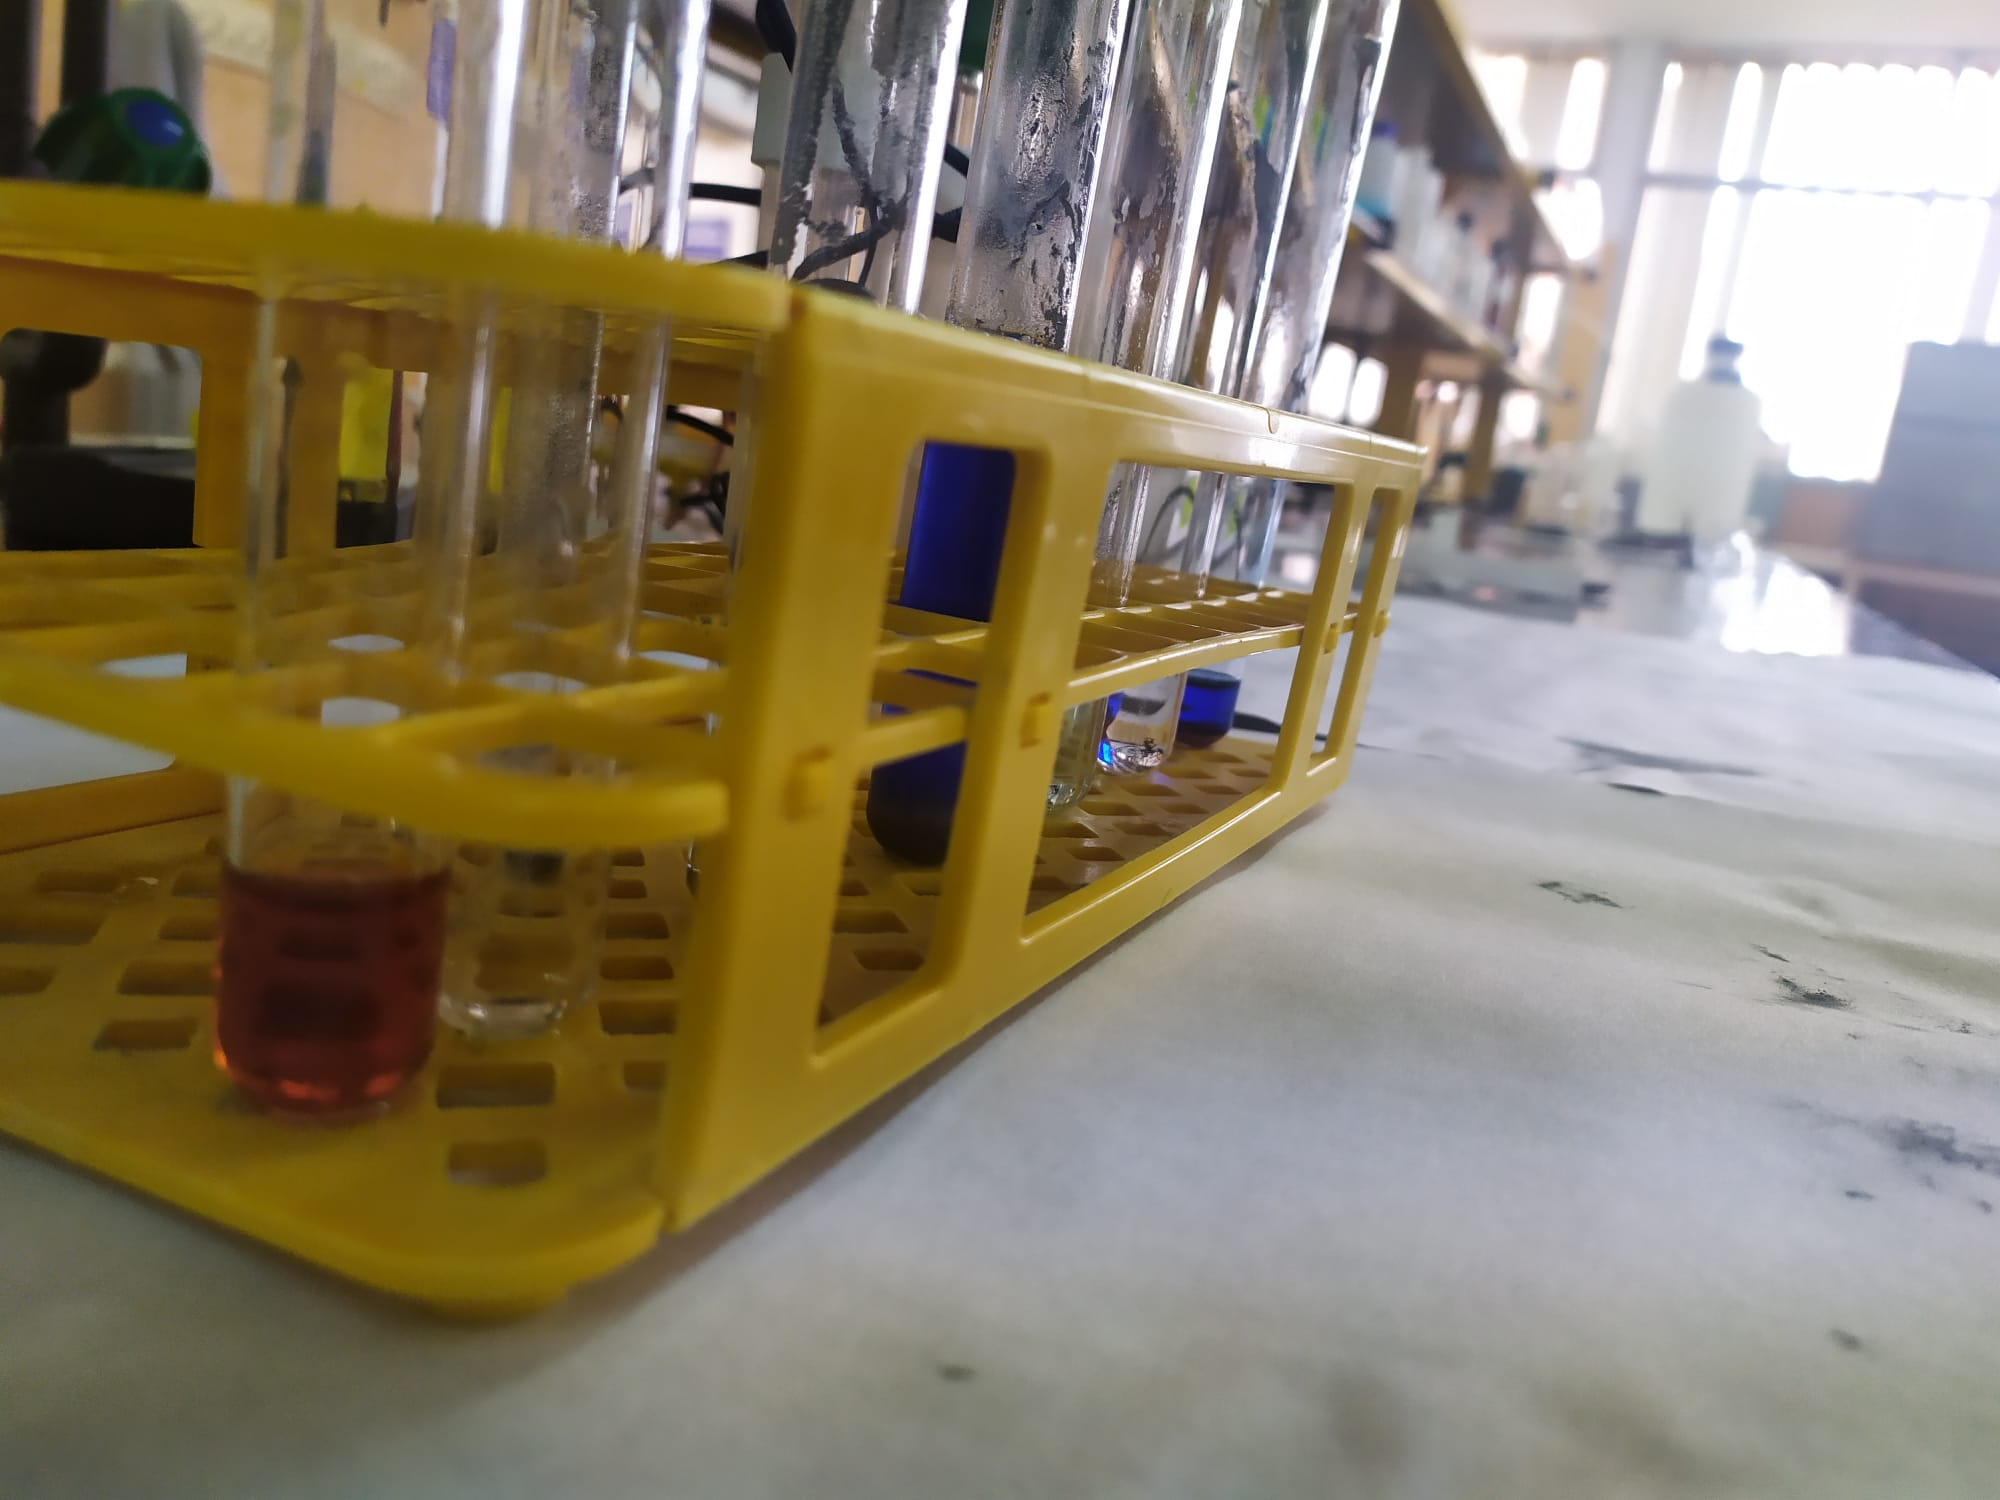
\includegraphics[width=0.6\textwidth]{prac5/Aesthetic.jpeg}
\end{figure}
\begin{figure}[h]
    \centering
    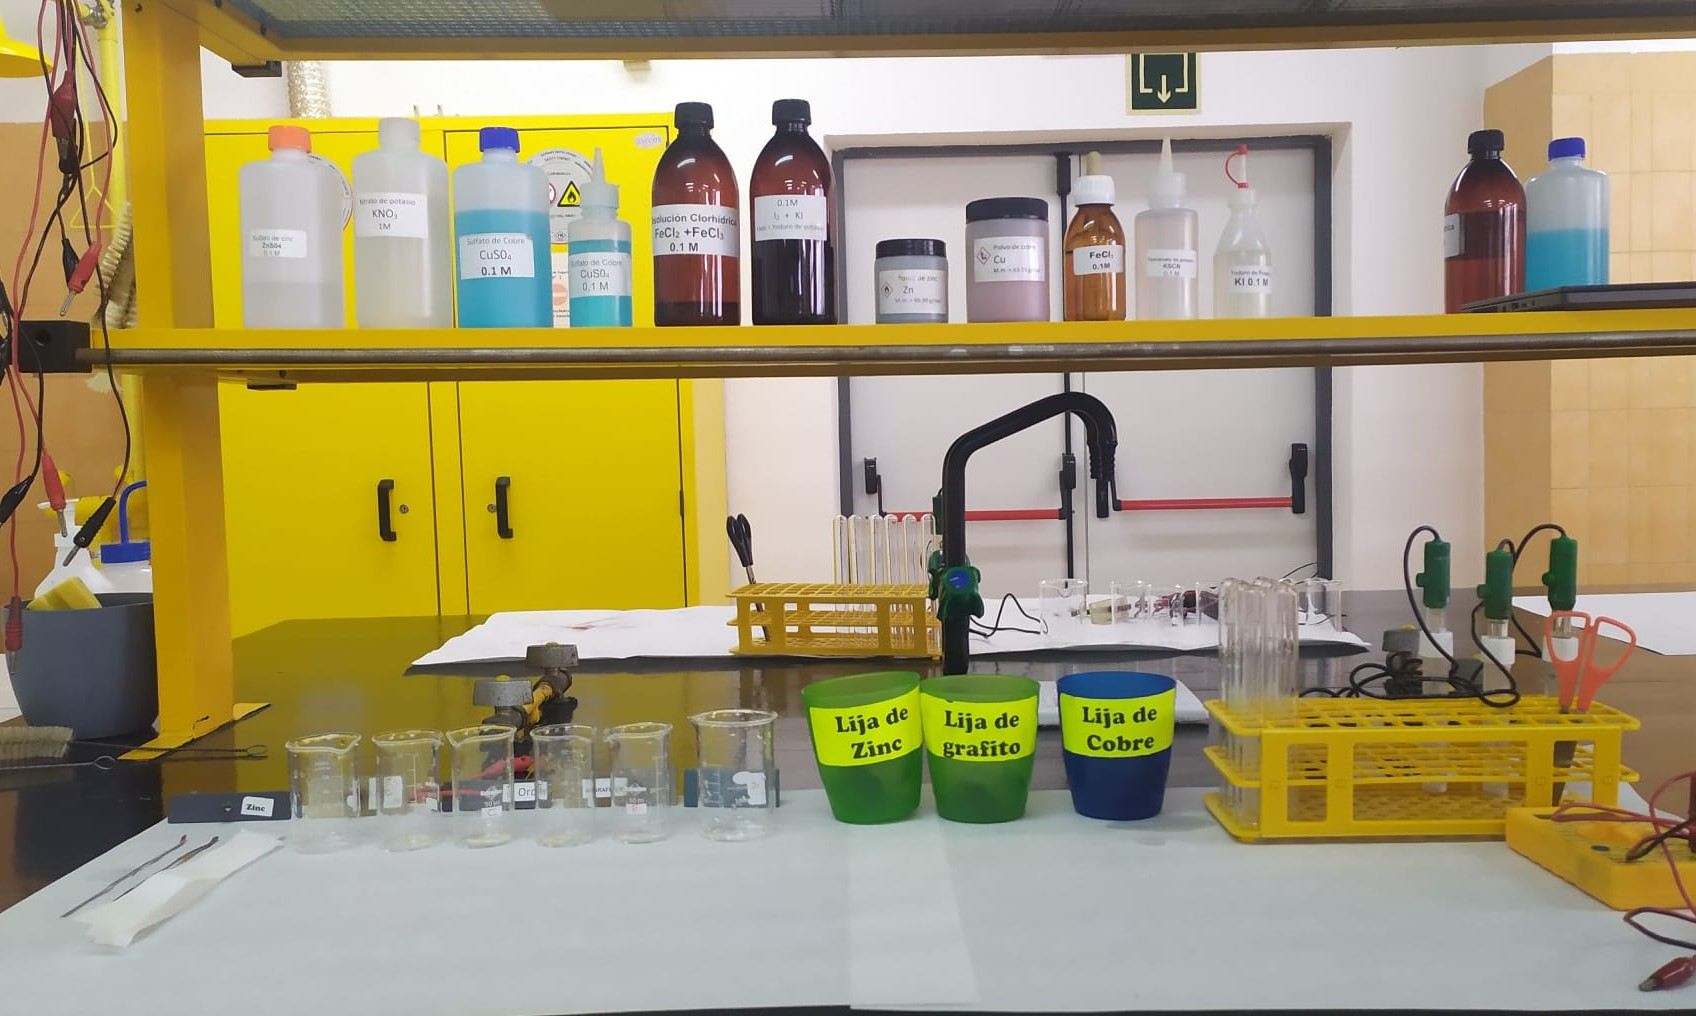
\includegraphics[width=0.6\textwidth]{prac5/Inventario 5 todo.jpeg}
\end{figure}
\section{Introducción}
\noindent Esta práctica consta de tres partes. En primer lugar, mediremos la diferencia de potencial que hay en una pila, seguidamente mediremos los potenciales de diferentes pares redox frente a un electrodo de referencia y, finalmente, realizaremos ensayos redox cualitativos.

\vspace{0.4cm}
\section{Inventario}
Para esta práctica hemos usado:

\begin{multicols}{2}
    \begin{itemize}
        \item Vasos de precipitados
        \item Papel de filtro
        \item Tijeras
        \item Espátulas metálicas
        \item Multímetro (y cables)
        \item Electrodos (grafito, oro y cinc)
        \item Electrodo de referencia (\ce{AgCl}/\ce{Ag})
        \item Polvo de cinc y cobre
        \item Lijas de grafito, cobre y cinc
        \item \ce{CuSO4} $1M$
        \item \ce{FeCl3} $0.1M$ y \ce{FeCl3} $0.1M$
        \item \ce{ZnSO4} $1M$
        \item \ce{I2} + \ce{KI} $1M$
        \item \ce{KI} $0.1M$
        \item \ce{KSCN}
        \item \ce{NH3} concentrado
    \end{itemize}
\end{multicols}

\begin{figure}[H]
    \centering
    \hspace*{-3cm}
        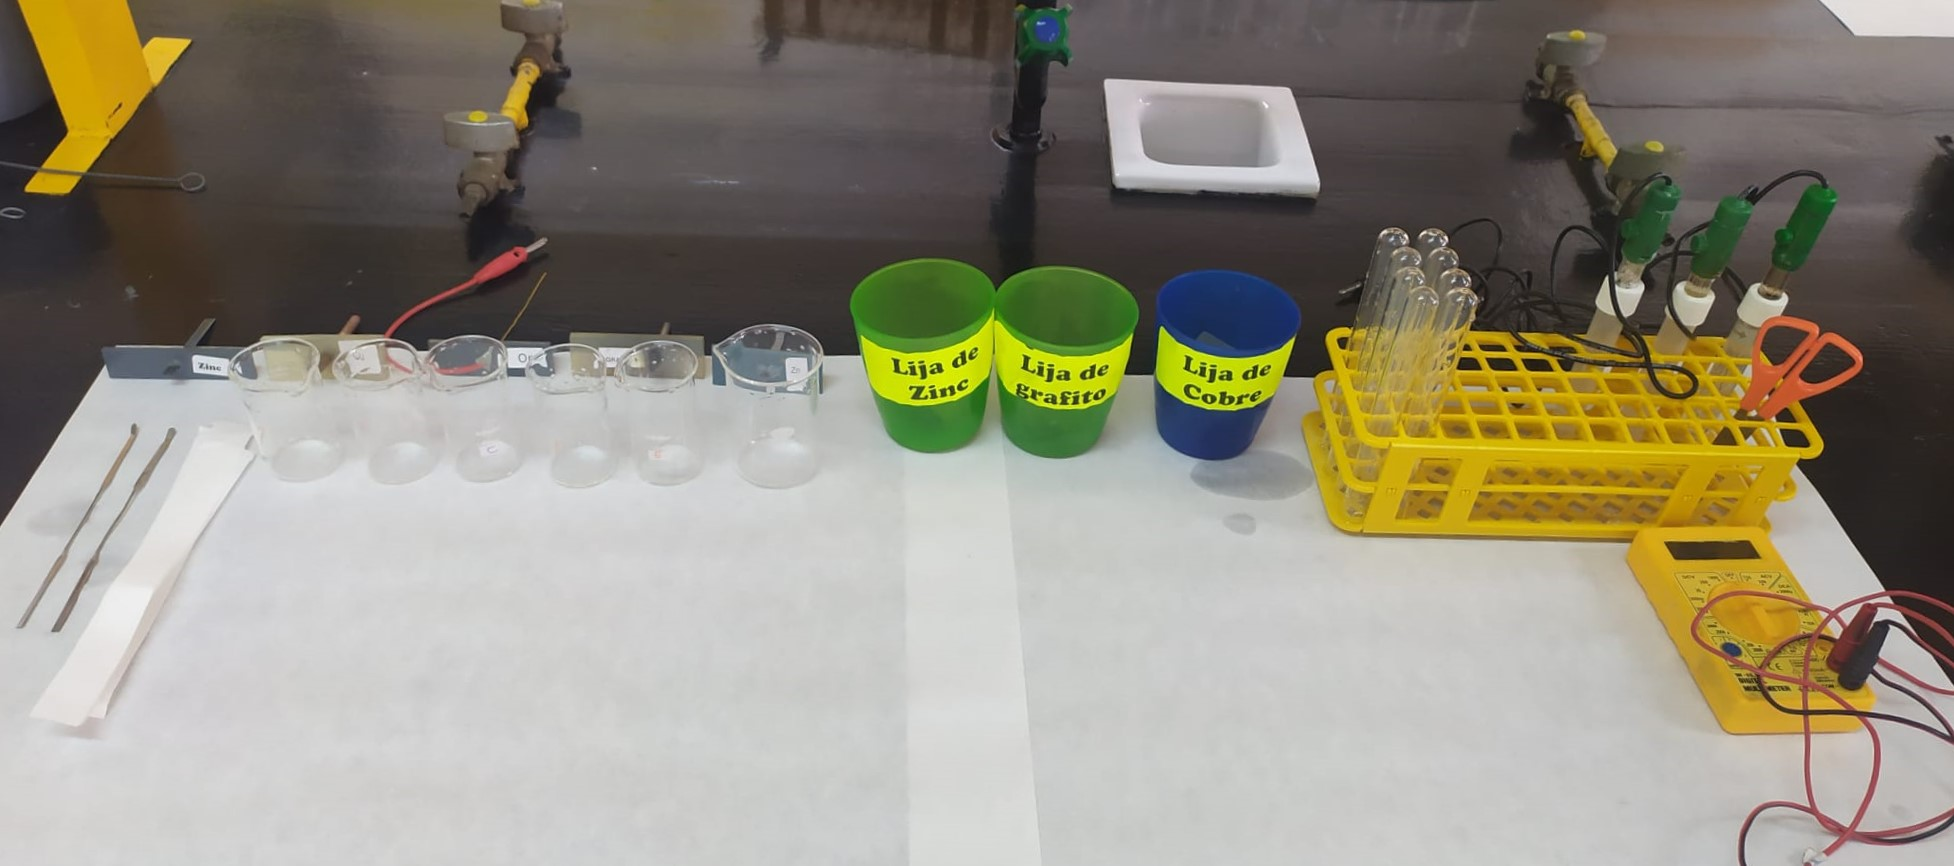
\includegraphics[scale = 0.2]{prac5/Material.jpeg}
        \includegraphics[scale = 0.087]{prac5/Líquidos_empleados.jpeg}
    \hspace*{-3cm}
    \caption{Material utilizado a lo largo de la práctica}
\end{figure}

\clearpage

\section{Procedimiento}
\subsection{Medición de la diferencia de potencial de una pila}
\noindent Colocaremos las 4 soluciones de 40 \si{ml} en vasos de precipitado distintos, marcándolas como A,B,C y D:
\begin{enumerate}[A -]
\item CuSO4 1M
\item Disolución clorhídrica 0,1 M en FeCl3 y FeCl2
\item ZnSO4 0,1 M
\item I2 + KI 0,1 M
\end{enumerate}

\noindent Ahora, vamos a crear diferentes pilas según los pares redox que conectemos y los electrodos que utilicemos:

\begin{enumerate}
\item A con electrodo de Cu y B con electrodo de grafito
\item A con electrodo de Cu y B con electrodo de Au
\item A con electrodo de Cu y C con electrodo de Zn
\item A con electrodo de Cu y D con electrodo de grafito
\item B con electrodo de grafito y C con electrodo de Zn
\item B con electrodo de Au y D con electrodo de grafito
\item C con electrodo de Zn y D con electrodo de grafito
\end{enumerate}

\noindent Anotamos los diferentes potenciales obtenidos para los pares de disoluciones A-D:

\begin{table}[H]
\centering
\begin{tabular}{ccc}
\rowcolor[HTML]{9698ED} 
\textbf{Pila} & \textbf{$\Delta V_{\text{teórico}}$ (\si{V})} & \multicolumn{1}{l}{\cellcolor[HTML]{9698ED}\textbf{$\Delta V_{\text{experimental}}$ (\si{V})}} \\
\rowcolor[HTML]{DAE8FC} 
\textbf{B - A (grafito)} & $0.43$ & $0.41$ \\
\textbf{B - A (oro)} & $0.43$ & $0.42$ \\
\rowcolor[HTML]{DAE8FC} 
\textbf{B - C} & $1.53$ & $1.41$ \\
\textbf{B - D} & $0.23$ & $0.18$ \\
\rowcolor[HTML]{DAE8FC} 
\textbf{A - C} & $1.10$ & $0.94$ \\
\textbf{A - D} & $0.20$ & $0.23$ \\
\rowcolor[HTML]{DAE8FC} 
\textbf{C - D} & $1.30$ & $1.25$
\end{tabular}
\label{potencial}
\end{table}
\noindent Destacar como el electrodo de oro posee una menor resistencia eléctrica y por ello se acerca más al valor teórico.
\clearpage

\subsection{Medida de los potenciales de diferentes pares frente a un electrodo de
referencia}
\noindent Para realizar estas medidas, cogeremos el vaso de precipitados restante e
introduciremos 40 mL de una disolución saturada de cloruro de potasio, en la que
sumergiremos el electrodo de referencia \ce{AgCl/Ag}, conectándolo al polo negativo
de nuestro multímetro.\\\\
A continuación, formaremos 4 pilas nuevas, formadas cada una por la nueva
disolución y realizando combinaciones con las disoluciones A-D, con el fin de
medir cada uno de los potenciales.

\begin{table}[H]
\centering
\begin{tabular}{cc}
\rowcolor[HTML]{9698ED} 
\textbf{Disolución} & \textbf{\Delta V} \\
\rowcolor[HTML]{DAE8FC} 
\textbf{A} & $0.08$ \\
\textbf{B} & $0.44$ \\
\rowcolor[HTML]{DAE8FC} 
\textbf{C} & $-0.9$ \\
\textbf{D} & $0.32$
\end{tabular}
\caption{Electrodo de referencia}
\label{referencia}
\end{table}

\subsection{Ensayos redox cualitativos}
\noindent Mediante el uso de tubos de ensayo y diferentes reactivos sólidos, llevamos a cabo estas reacciones, anotando los cambios observados.
\begin{enumerate}
\item 20 gotas de la disolución de FeCl3 0,1 M con 20 gotas de KI 0,1 M
\item 20 gotas de KI 0,1 M con 20 gotas de ZnSO4 0,1 M
\item Polvo de Zn con 20 gotas de la disolución de FeCl3 0,1 M. En este caso, ensayamos la presencia de iones Fe3+ con unas gotas de KSCN 0,1 M
\item 20 gotas de la disolución de FeCl3 con unas gotas de KSCN y polvo de Zn
\item Polvo de Zn con 20 gotas de la disolución de CuSO4. Ensayamos la presencia de iones Cu2+ con unas gotas de disolución concentrada de NH3.
\item 20 gotas de CuSO4 con 20 gotas de ZnSO4
\item Polvo de Zn con 20 gotas de una disolución de HCl 6M
\item Polvo de Cu con 30 gotas de una disolución de HCl 6M. Ensayamos la presencia de iones Cu2+ con unas gotas de disolución concentrada de NH3
\end{enumerate}


\clearpage
\section{Cuestiones}
\noindent\textcolor{BlueViolet}{\textbf{\textit{a) Exprese mediante ecuaciones los procesos redox que tienen lugar en cada una de las pilas formadas en el apartado 1. De acuerdo con los potenciales y polaridades observados, ordene los diferentes pares redox según su poder oxidante creciente.}}}\\
\begin{enumerate}
\item A con electrodo de Cu y B con electrodo de grafito \\
    Cátodo - (\ce{2Fe^{3+} + 3e^- <=> 2Fe^{2+}})\cdot 2 \\
    Ánodo  - (\ce{Cu <=> Cu^{2+} + 2e^-})\cdot 3 \\
    $\overline{\ce{4Fe^{3+} + 3Cu <=> 3Cu^{2+} + 4Fe^{2+}}}$
\item A con electrodo de Cu y C con electrodo de Zn \\
    Cátodo - \ce{2Fe^{3+} + 2e^- <=> 2Fe^{2+}} \\
    Ánodo  - \ce{Zn <=> Zn^{2+} + 2e^-} \\
    $\overline{\ce{2Fe^{3+} + Zn <=> Zn^{2+} + 2Fe^{2+}}}$
\item A con electrodo de Cu y D con electrodo de grafito \\
    Cátodo - \ce{Cu^{2+} + 2e^- <=> Cu} \\
    Ánodo  - \ce{2I^- <=> I2 + 2e^-} \\
    $\overline{\ce{Cu^{2+} + 2I^- <=> Cu + I2}}$
\item B con electrodo de grafito y C con electrodo de Zn \\
    Cátodo - (\ce{Fe^{3+} + e^- <=> Fe^{2+}})\cdot 2 \\
    Ánodo  - \ce{Zn <=> Zn^{2+} + 2e^-} \\
    $\overline{\ce{2Fe^{3+} + Zn <=> 2Fe^{2+} + Zn^{2+}}}$
\item B con electrodo de Au y D con electrodo de grafito \\
    Cátodo - (\ce{Fe^{3+} + e^- <=> Fe^{2+}})\cdot 2 \\
    Ánodo  - \ce{2I^- <=> I2 + 2e^-} \\
    $\overline{\ce{2Fe^{3+} + 2I^- <=> 2Fe^{2+} + I2}}$
\item C con electrodo de Zn y D con electrodo de grafito \\
    Cátodo - \ce{I2 + 2e^- <=> 2I^-} \\
    Ánodo  - \ce{Zn <=> Zn^{2+} + e^-} \\
    $\overline{\ce{I2 + Zn <=> 2I^- + Zn^{2+}}}$
\end{enumerate}
\clearpage

\noindent\textcolor{BlueViolet}{\textbf{\textit{b) Ordene los pares de mayor a menor potencial de acuerdo con las medidas del apartado 2. y compare el resultado con la ordenación establecida en el apartado 1. Compare los valores de potencial obtenidos en el apartado 2 con los esperados según los datos del Handbook.}}}\\\\
\noindent Siguiendo los datos acerca de los potenciales que hemos tomado en la tabla \ref{referencia}, podemos ordenar las pilas según el poder oxidante en sentido creciente:
\[\textbf{\boxed{\text{C <\ A <\ D <\ B}}}\]
Esta ordenación concuerda con la obtenida en la cuestión anterior, por lo que confirma la certeza de los datos obtenidos. Para asegurarnos más, comparamos con los datos existentes en el \textquote{\textit{CRC Handbook of Chemistry and Physics}}:
\begin{table}[H]
\centering
\begin{tabular}{ccc}
\rowcolor[HTML]{9698ED} 
\textbf{Reacción} & \textbf{$\Delta V_{\text{teórico}}$} & \cellcolor[HTML]{9698ED}\textbf{$\Delta V_{\text{experimental}}$} \\
\rowcolor[HTML]{DAE8FC} 
\textbf{A} & $-0.16$ & $+0.08$ \\
\rowcolor[HTML]{FFFFFF} 
\textbf{B} & $+0.77$ & $+0.44$ \\
\rowcolor[HTML]{DAE8FC} 
\textbf{C} & $-0.76$ & $-0.9$ \\
\textbf{D} & $+0.54$ & $+0.32$
\end{tabular}
\label{pot5}
\end{table}
\noindent\textcolor{BlueViolet}{\textbf{\textit{c) Discuta los resultados obtenidos en el apartado 3 en base a los valores de potencial obtenidos en los apartados anteriores. Escriba las ecuaciones correspondientes en los casos en los que hubo reacción.}}}

\begin{changemargin}{1.5cm}{0cm}
\noindent
\begin{enumerate}[\text{Reacción} 1 - ]
    \item El \ce{Fe^{3+}} se reduce y el \ce{I^-} se oxida. Se observa un color rojo en la reacción.\\
    \ce{2Fe^{3+} + 2I^- <=> 2Fe^{2+} + I2}
    \item El \ce{Zn^{2+}} se reduce y el \ce{I^-} se oxida. No es espontánea. \\
    \ce{Zn^{2+} + 2I^- <=> Zn + I2}
    \item Se observa color rojizo. Aparición de burbujas de gas.\\
    \ce{KSCN + FeCl3 + 5H2O -> [Fe(NCS)(H2O)5]^{2+} + 2Cl^- + KCl}
    \item El polvo de cinc precipita.
    \item No sucede nada, lo que implica una ausencia de iones \ce{Cu^{2+}}.
    \item No sucede nada.
    \item Se observa la aparición de burbujas de gas. Aumento de la temperatura.
    \item Se observa un coloro azul en la reacción al añadir \ce{NH3} \\
    \ce{Cu^{2+} + 4NH3 <=> Cu(NH3)4^{2+}}
\end{enumerate}
\end{changemargin}

% PRÁCTICA 6
\chapter[Práctica 6]{6. Síntesis del ácido acetilsalicílico}
\thispagestyle{empty}
\vspace{1cm}
\begin{figure}[h]
    \centering
    \hspace*{-0.2cm}
    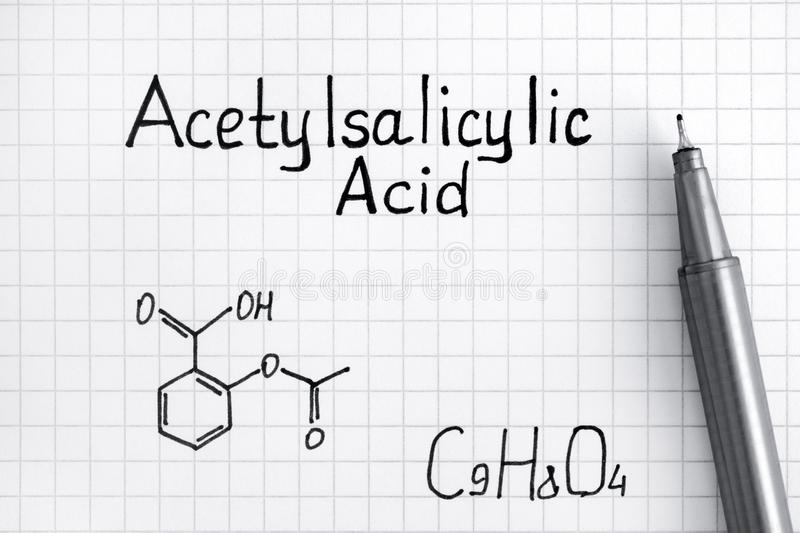
\includegraphics[width=1\textwidth]{fotos/fórmula-química-del-ácido-acetilsalicílico-con-la-pluma-114646429.jpg}
    \hspace*{-0.4cm}
\end{figure}
\section{Introducción}
\vspace{0.2cm}
\noindent En esta práctica vamos a hacer una síntesis del ácido acetilsalicílico (también conocido como Aspirina) partiendo de ácido salicílico, es un proceso fácil pero requiere bastante tiempo y atención. \\\\
A lo largo de esta práctica prepararemos disoluciones, las trabajaremos al baño maría y pasaremos un par de veces por el proceso de cristalización que lo podemos ver visualmente en la Figura \ref{fig:crist}.

\vspace{0.4cm}

\begin{figure}[h]
    \centering
    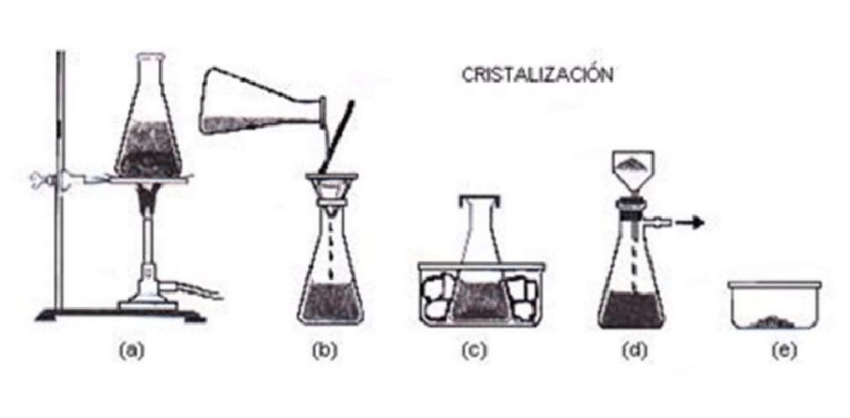
\includegraphics[scale = 0.5]{Figura-3-Proceso-general-de-cristalizacion-por-pasos-Fuente.png}
    \caption{Imagen de un proceso de cristalización}
    \label{fig:crist}
\end{figure}

\vspace{0.6cm}

\noindent En el apartado \ref{proc} explicaremos más detalladamente el desarrollo de la práctica.

\clearpage
\section{Inventario}  
\noindent En esta práctica contamos con:
\begin{multicols}{2}
    \begin{itemize}
        \item 4 tubos de ensayo 
        \item 1 picnómetro
        \item 3 vasos de precipitados
        \item Un erlemmeyer
        \item 2 pipetas
        \item Una varilla
        \item Una probeta
        \item Un frasco lavador
        \item Un matraz Kitasatos
        \item Un embudo Büchner
        \item 2 vidrios de reloj
        \item Una placa calefactora
        \item Una espátula
        \item Una báscula
        \item Un matraz cristalizador
        \item Un termómetro
        \item Etanol
        \item Tricloruro de hierro
        \item Ácido salicílico
        \item Unos guantes de silicona
    \end{itemize}
\end{multicols}

\vspace{0.8cm}
\noindent Como bien podemos ver en las siguientes fotografías.
\vspace{0.4cm}

\begin{figure}[h]
    \centering
    \hspace*{-2.3cm}
        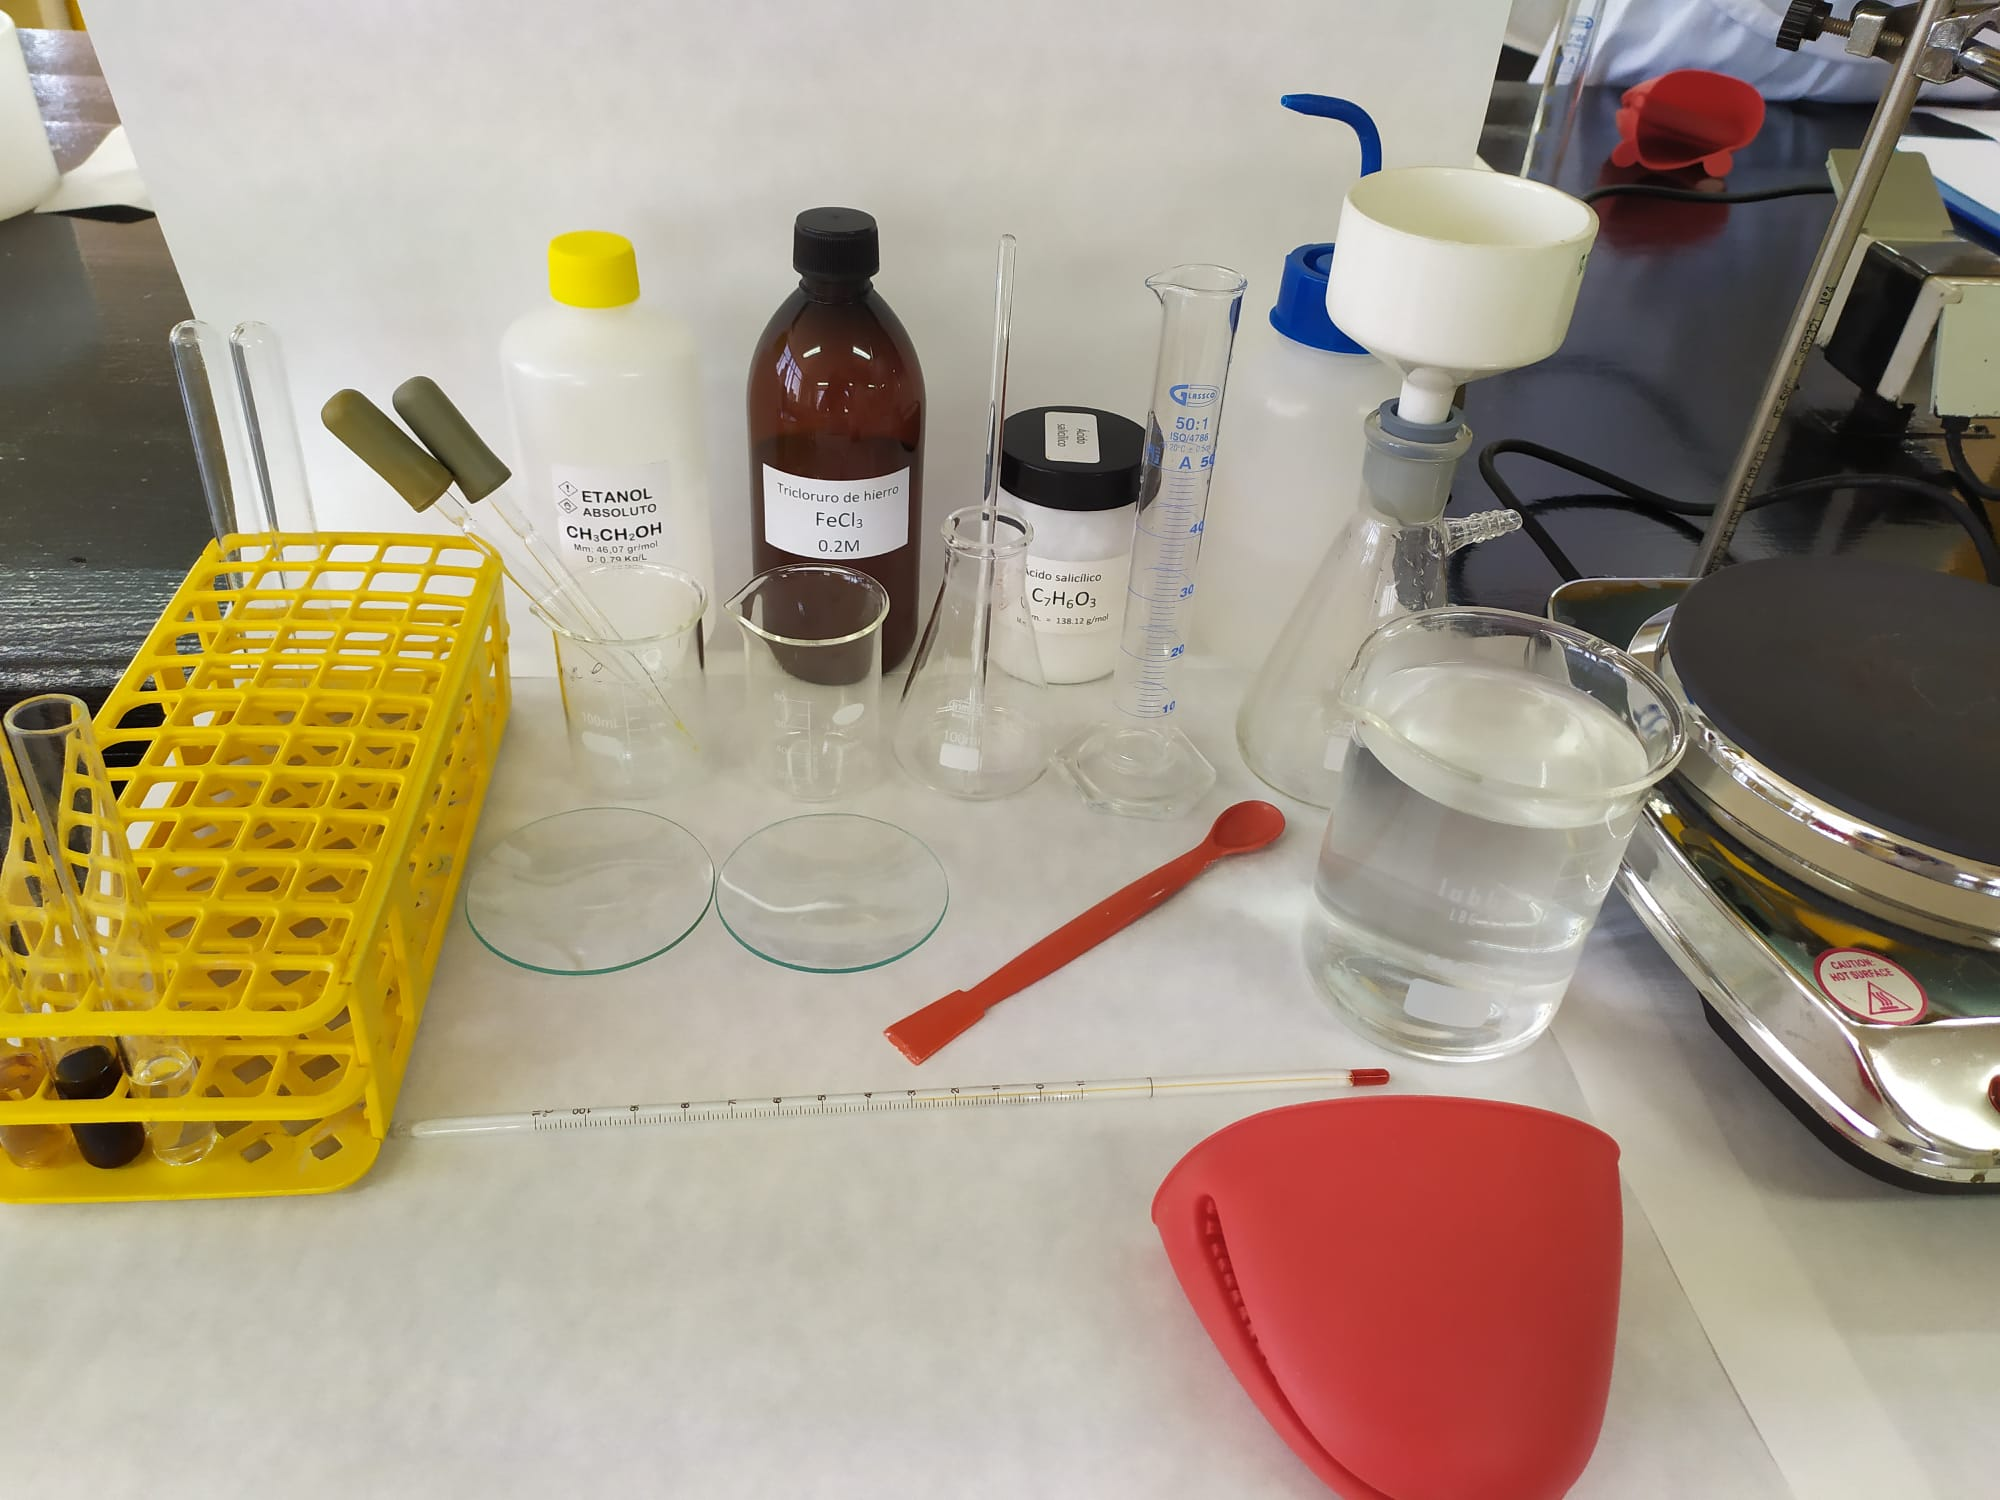
\includegraphics[scale = 0.1]{fotos/set6-1.jpeg}
        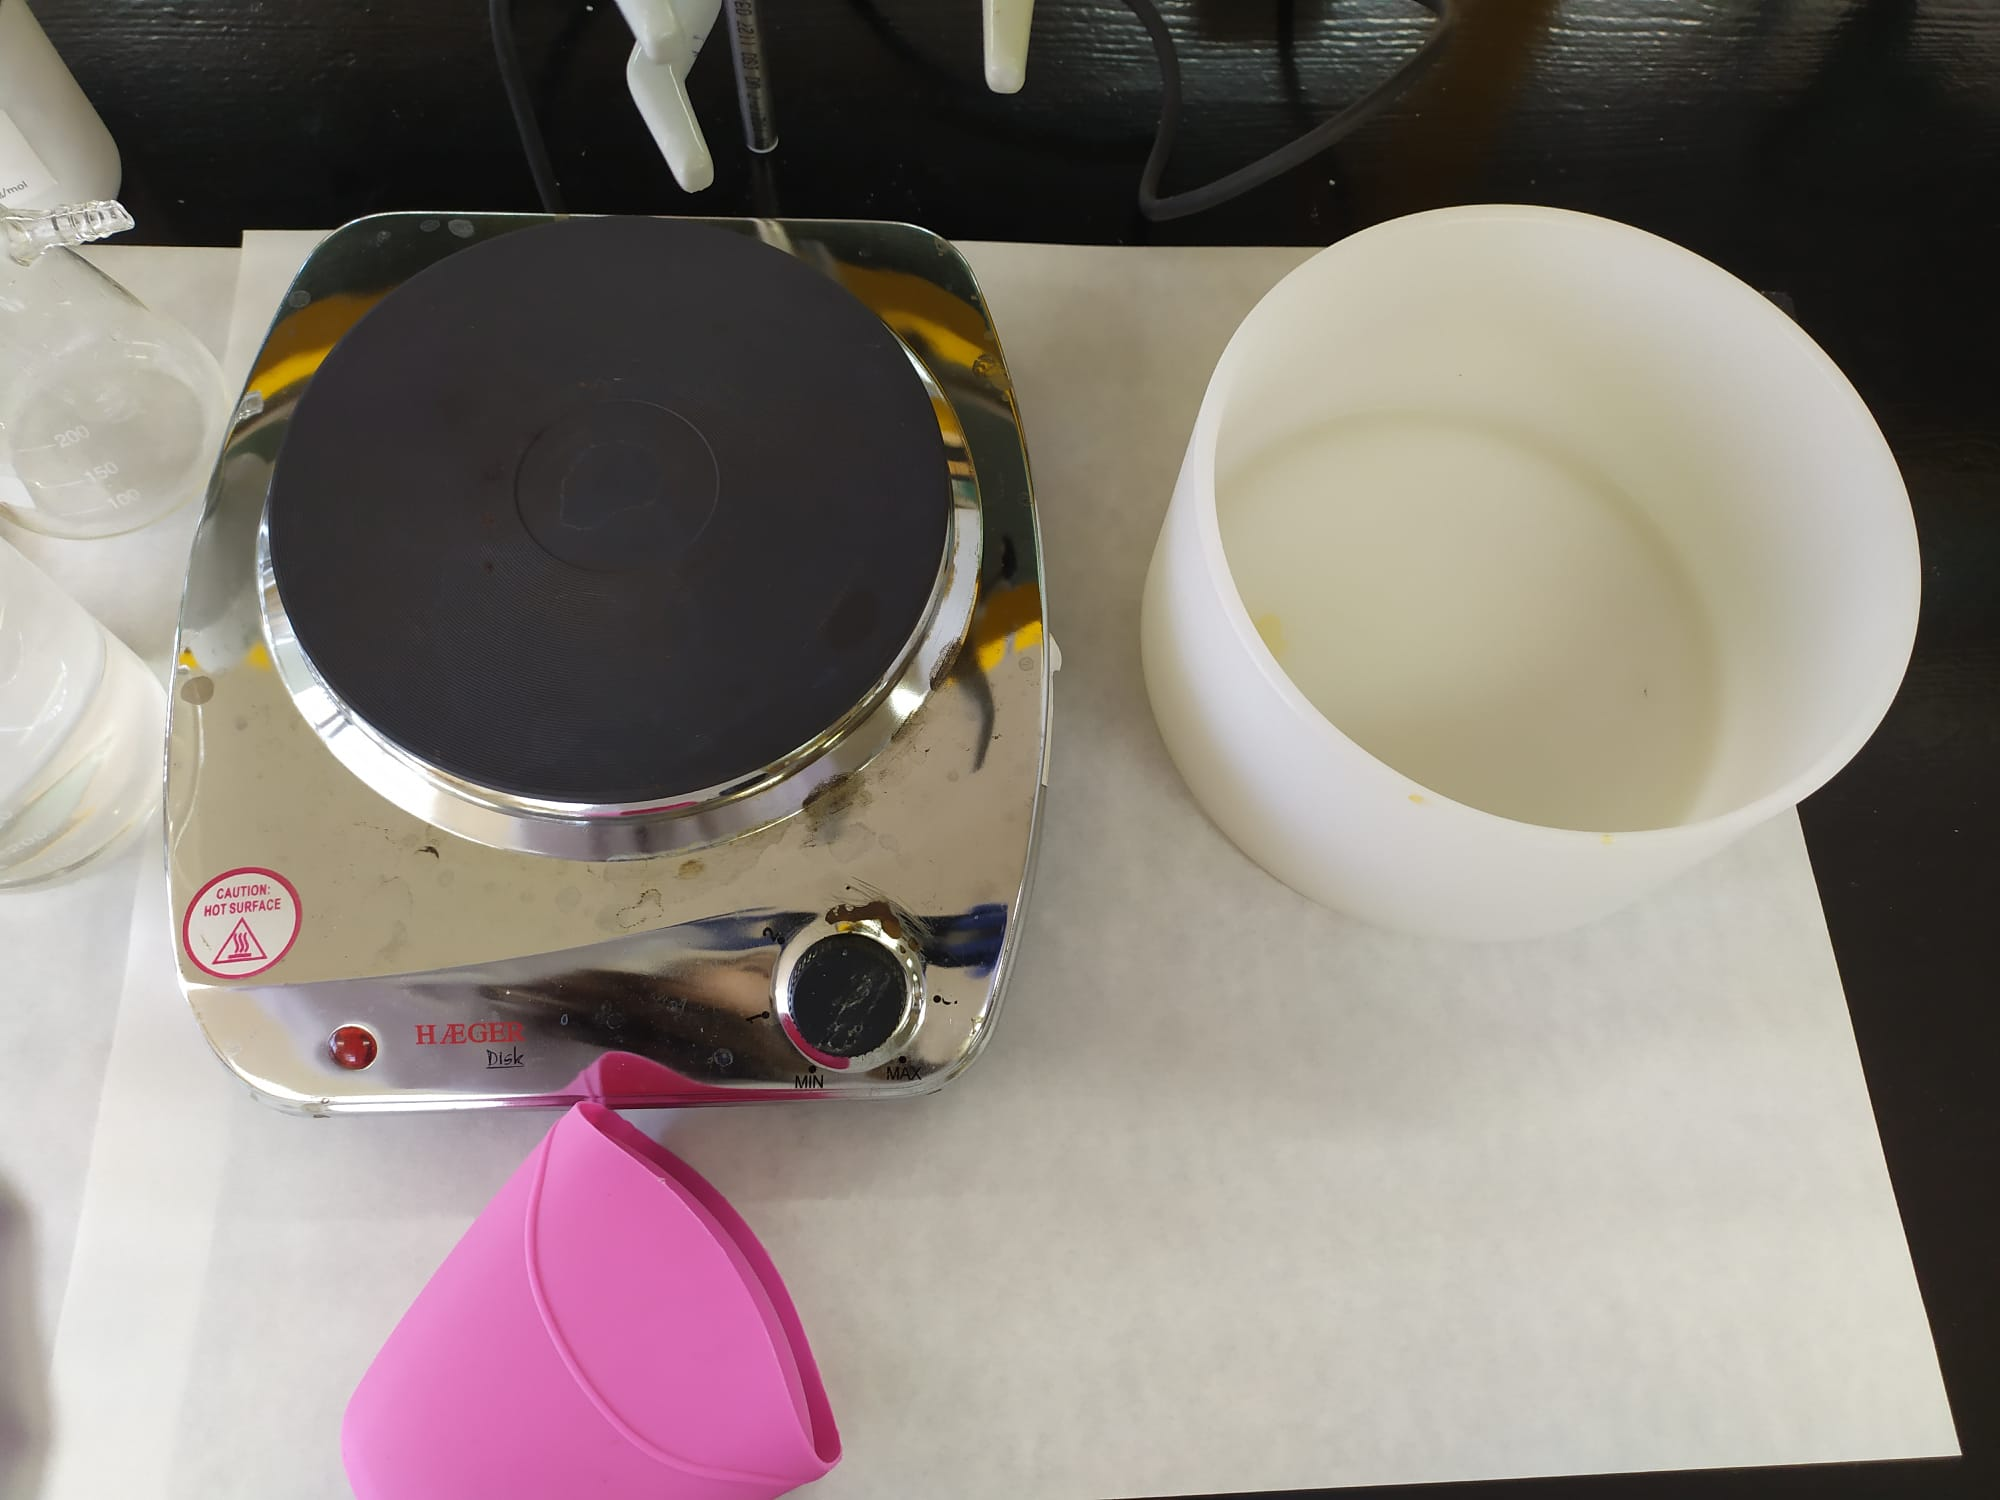
\includegraphics[scale = 0.1]{fotos/set6-2.jpeg}
    \hspace*{-2.3cm}
    \caption{Material de la práctica}
\end{figure}

\clearpage

\section{Procedimiento}\label{proc}
\noindent En primer lugar, tenemos que poner a calentar un vaso grande con agua en la placa calefactora para poder usar el baño maría. Cuando esté muy caliente pero sin necesidad de hervir, pondremos la disolución previamente preparada: hemos pesado 6g exactos de ácido salicílico en un matraz erlenmeyer y le hemos añadido 8 mL de anhídrido acético y 10 gotas de ácido sulfúrico concentrado. 

\vspace{0.2cm}

\noindent Una vez puesta la disolución al baño maría, la tendremos ahí alrededor de unos 20 minutos mientras que con una varilla la vamos removiendo para conseguir completar la reacción de la mezcla.

\vspace{0.2cm}

\noindent Tras los 20 minutos, agregamos poco a poco 25 mL de agua muy fría (destilada), para después ponerlo en el matraz cristalizador con hielo picado durante unos 10 minutos, hasta que la precipitación se complete.

\vspace{0.2cm}

\noindent Una vez se da la cristalización, separamos el precipitado del líquido mediante filtración al vacío durante 10 minutos más o menos. También lavaremos con agua fría el precipitado para que sea lo más puro posible.

\vspace{0.2cm}

\noindent A continuación, separaremos un poco de precipitado para realizar la prueba de fenoles al final de la práctica y el resto lo pasaremos a un vaso de precipitados de 100 mL para disolverlos con 15 mL de alcohol etílico para volver a calentarlo al baño maría hasta que ya no veamos el precipitado. Mientras hacemos esto, calentamos 50 mL de agua (destilada). Una vez sacado el vaso de precipitados le añadimos el agua que estábamos calentando, y cubrimos la disolución con un vidrio reloj (colocado como en la Figura \ref{fig:prec} hasta que se enfríe la mezcla y que consigamos una completa cristalización. Nosotros en un principio la dejamos enfriar a temperatura ambiente, pero debido al lento proceso, lo metimos en el cristalizador con hielo picado para que el proceso de precipitación tuviera lugar más rápidamente.


\vspace{0.4cm}

\begin{figure}[h]
    \centering
    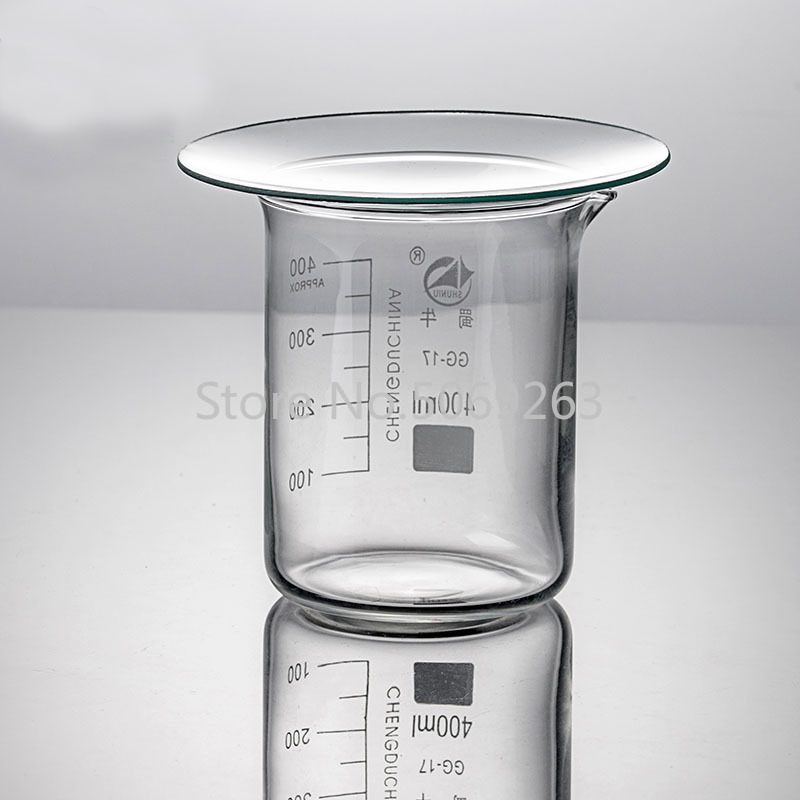
\includegraphics[scale = 0.12]{fotos/Plato-de-reloj-de-vidrio-de-laboratorio-cubierta-de-vaso-duro-en-forma-de-c-pula.jpg}
    \caption{Imagen de un vaso de precipitados con un vidrio reloj}
    \label{fig:prec}
\end{figure}

\vspace{0.4cm}

\noindent Una vez precipitado, volvemos a filtrar al vacío y los cristales formados los pasamos a un vaso limpio, y que ya hemos pesado (34.77 g), para después meterlo a la estufa con la finalidad de secar los cristales de ácido acetilsalicílico. Sacaremos el vaso de precipitados cada 5 minutos para pesarlo, hasta que dicho peso sea constante (esto último no vamos a poder hacerlo bien ya que para que la pesada sea constante tendríamos que esperar por lo menos hasta el día siguente).

\vspace{0.3cm}

\begin{table}[h]
    \centering
\begin{tabular}{ | c | c | } 
    \hline
    \multicolumn{2}{ |c| }{Resultados} \\
    \hline
    $T_1$ $(g)$ & 39.72 \\  
    $T_2$ $(g)$ & 39.6 \\  
    $T_3$ $(g)$ & 39.49 \\  
    $T_4$ $(g)$ & 39.35 \\  
    $T_5$ $(g)$ & 39.23 \\  
    $T_6$ $(g)$ & 39.12 \\  
    $T_7$ $(g)$ & 39.05 \\  
    \hline
\end{tabular}
    \caption{Tabla de los datos obtenidos  tras las mediciones}
    \label{tabla-gramos}
\end{table}

\vspace{0.3cm}

\noindent Por último, vamos a realizar la prueba de los fenoles. Para ello disolveremos en tres tubos de ensayo que ya contengan 5 mL de etanol algunos cristales de ácido salicílico (1), en otro tubo el producto sin purificar que habíamos reservado (2) y otro con el producto purificado obtenido al finalizar la práctica (3). Y les añadimos tres gotas de tricloruro.

\vspace{0.2cm}

-- En el \textbf{primer tubo} de ensayo obtenemos un color morado intenso porque reacciona con el ácido salicílico dando lugar a ese característico color.

\vspace{0.15cm}

-- En el \textbf{segundo tubo} encontraremos también un toque morado, pero prácticamente incoloro, ya que aún tenemos impurezas.

\vspace{0.15cm}

-- En el \textbf{tercer tubo} ya no hay casi morado, pero aún se aprecia un poco porque no hemos terminado correctamente el proceso y hay impurezas de ácido salicílico, que es lo que reacciona.



\vspace{0.2cm}
\noindent Por tanto, hemos conseguido llegar casi al ácido acetilsalicílico pero en esta prueba hemos podido observar que aún nos quedaría dejar la muestra más tiempo en la estufa.

\clearpage

\section{Cuestiones} 

\noindent Empezamos con 6 gramos de ácido salícilico, y terminamos con $\approx$ 3 gramos de ácido acetilsalicílico, por tanto obtenemos un rendimiento del 50$\%$

\vspace{0.3cm}

\noindent La reacción que se produce es $C_7H_6O_3 + C_4H_6O_3 \rightarrow C_9H_8O_4 + C_2H_4O_2$, y podemos observar que un mol de ácido salicílico reacciona con un mol de ácido acetilsalicílico, y sabemos que la masa final de producto es 39.05 - 34.77 = \underline{4.28 g}. Para calcular la masa teórica (para así sacar el rendimiento) deberemos pasar los 6 gramos iniciales de ácido salicílico a los gramos finales de ácido acetilsalicílico mediante factores de conversión:

\vspace{0.3cm}

\noindent Sabiendo que la masa molar de ácido acetilsalicílico es de 180 g/mol y la del ácido salicílico es de 138 g/mol ya podemos calcular la masa teórica:

\[ 6 ~ g \cdot \frac{1 ~ mol ~ C_7H_6O_3}{102 ~ g ~ C_7H_6O_3} \cdot \frac{180 ~ g ~ C_9H_8O_4}{1 ~ mol ~ C_9H_8O_4} = 7.82 ~ g ~ de ~ C_9H_8O_4\]

\noindent Una vez hallada la masa teórica, ya podemos calcular el rendimiento:

\[ Rendimiento = \frac{masa ~ real}{masa ~ teorica}\cdot{100} = \frac{4.28}{7.82}\cdot{100} = 54.73\% \]


\vspace{0.3cm}

%%%%%%%%%%%%%%%%%%%%%%%%%%VEEEEEEEEEEEEEERRRRRRRRRR

\noindent Podemos observar que hemos perdido casi la mitad de la masa inicial, debido a que el proceso ha sido más rápido de lo que debería, tendríamos que dejarlo una noche entera.


%%%%%%%%%%%%%%%%%%%%%%%%%%VEEEEEEEEEEEEEERRRRRRRRRR









% PRÁCTICA 7
\chapter[Práctica 7]{7. Estudio de la descomposición del \ce{H2S2O3}}
\thispagestyle{empty}
\vspace{1cm}
\begin{figure}[h]
    \centering
    \hspace*{-0.2cm}
    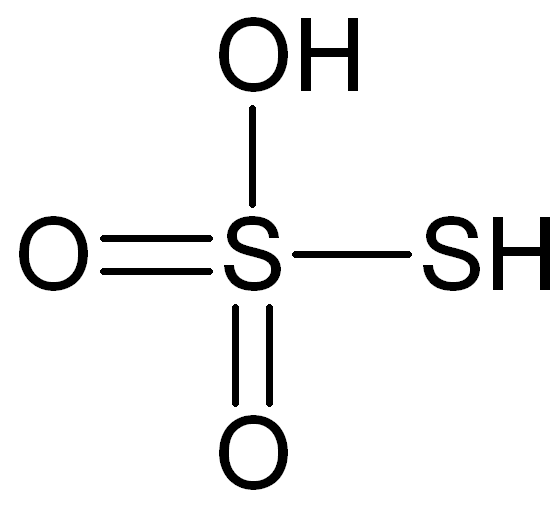
\includegraphics[width=0.8\textwidth]{prac7/Portada.png}
    \hspace*{-0.4cm}
\end{figure}
\section{Introducción}
\noindent En esta práctica, acidificaremos una disolución de tiosulfato (\ce{H2S2O3}) en la que precipitará azufre y enturbiará nuestras disolulciones. El fin es determinar el orden de esta reacción respecto al tiosulfato además de la velocidad inicial de reacción.\\ \\
\noindent Para ello variaremos la concentración inicial de uno de los reactivos y mantendremos las demás, analizando los datos en función de cuan rápido se produzca la reacción.

\section{Inventario}
Para esta práctica hemos usado:

\begin{itemize}
    \item 3 Buretas
    \item Tubo de ensayo
    \item Cronómetro
    \item 7 Vasos de precipitados ($100ml$)
    \item \ce{H2SO4} $0.5M$
    \item \ce{Na2S2O3} $0.3M$
    \item Frascos lavadores
\end{itemize}

\vspace{0.8cm}

\begin{figure}[H]
    \centering
    \hspace*{-3cm}
        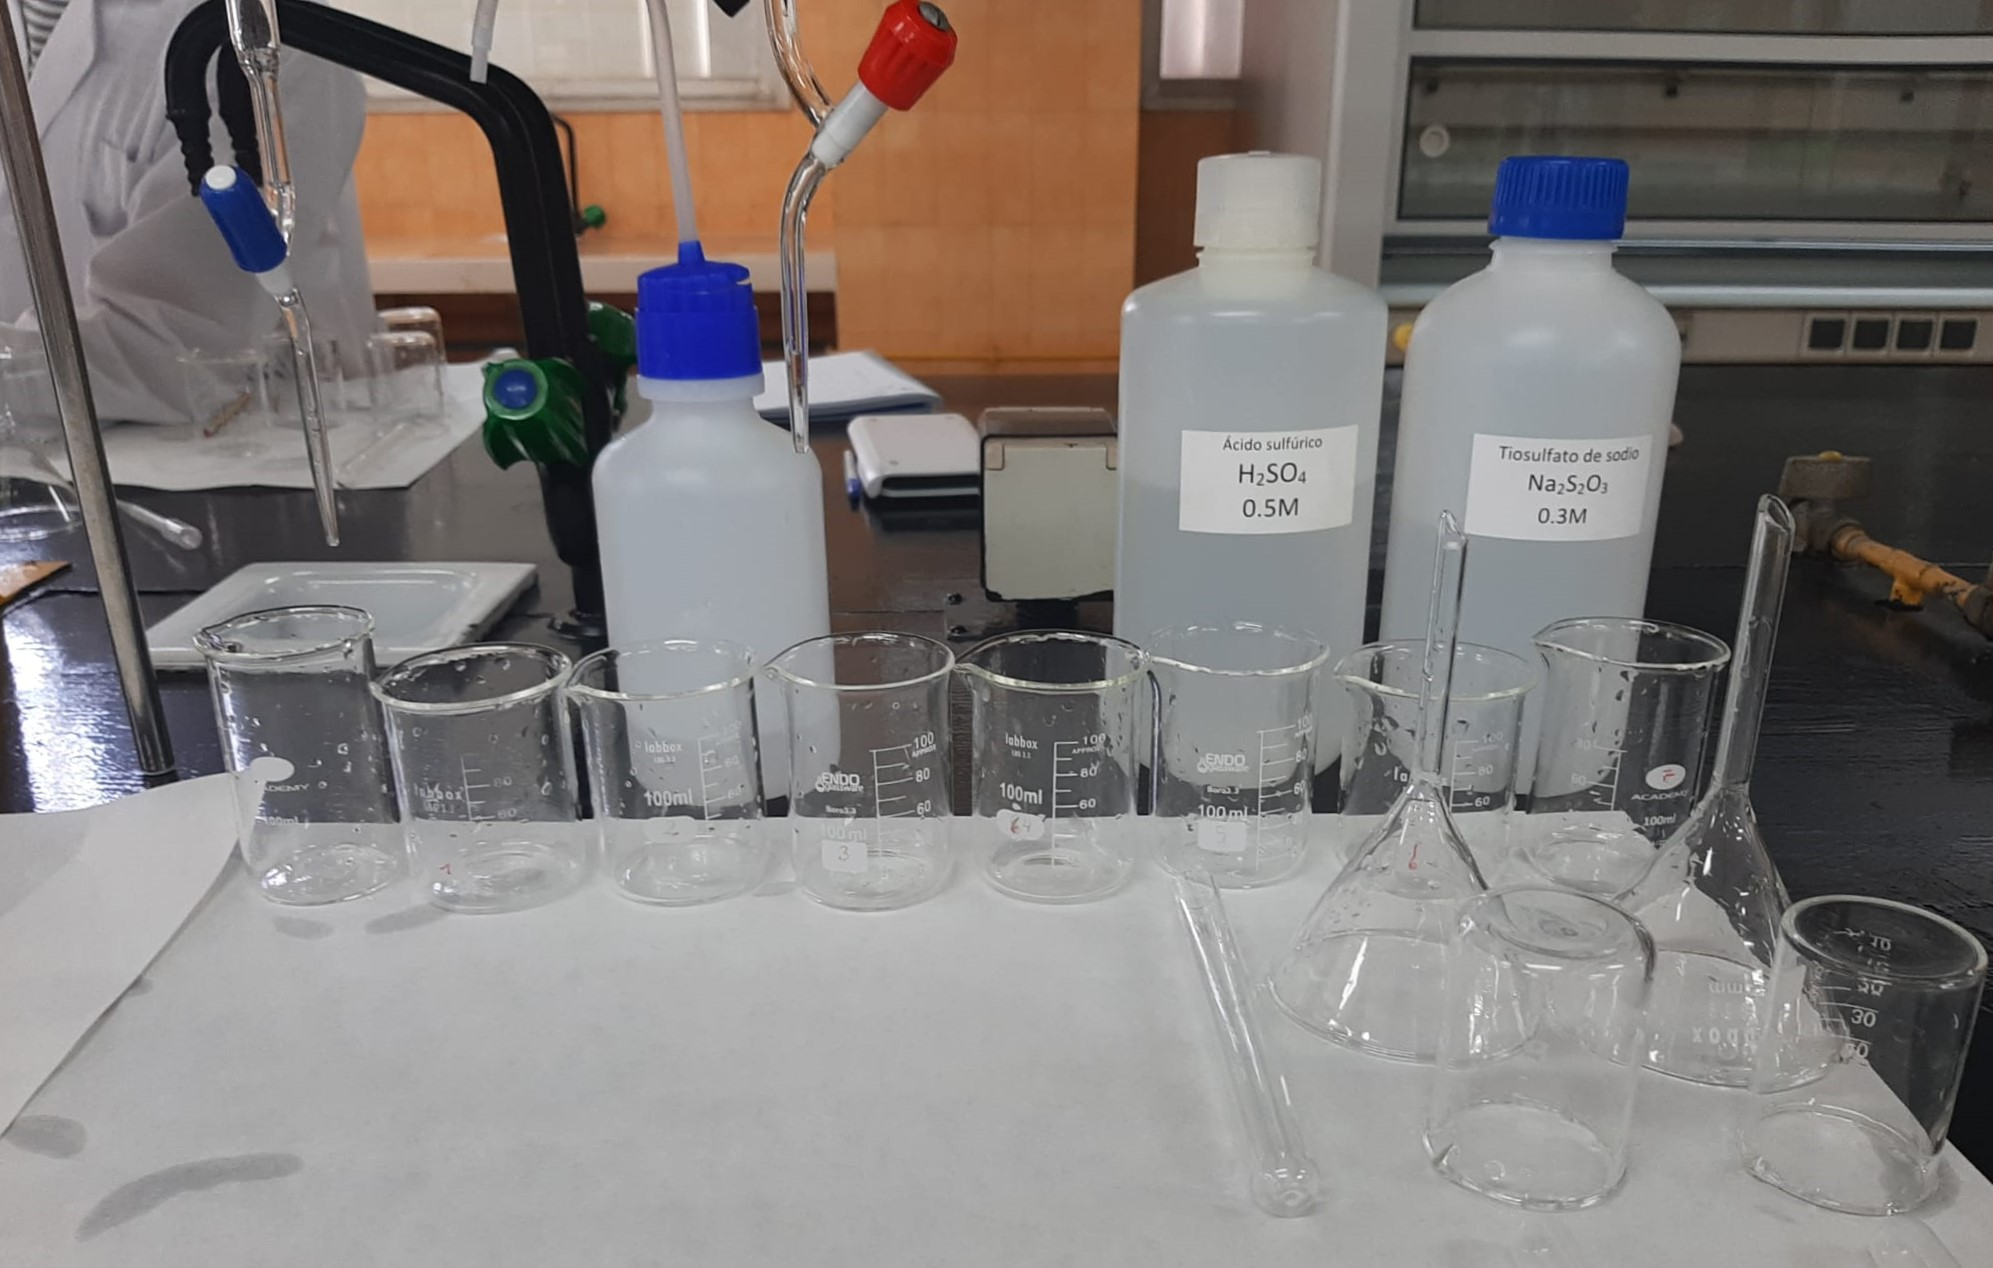
\includegraphics[scale = 0.2]{prac7/Inventario Todo.jpeg}
        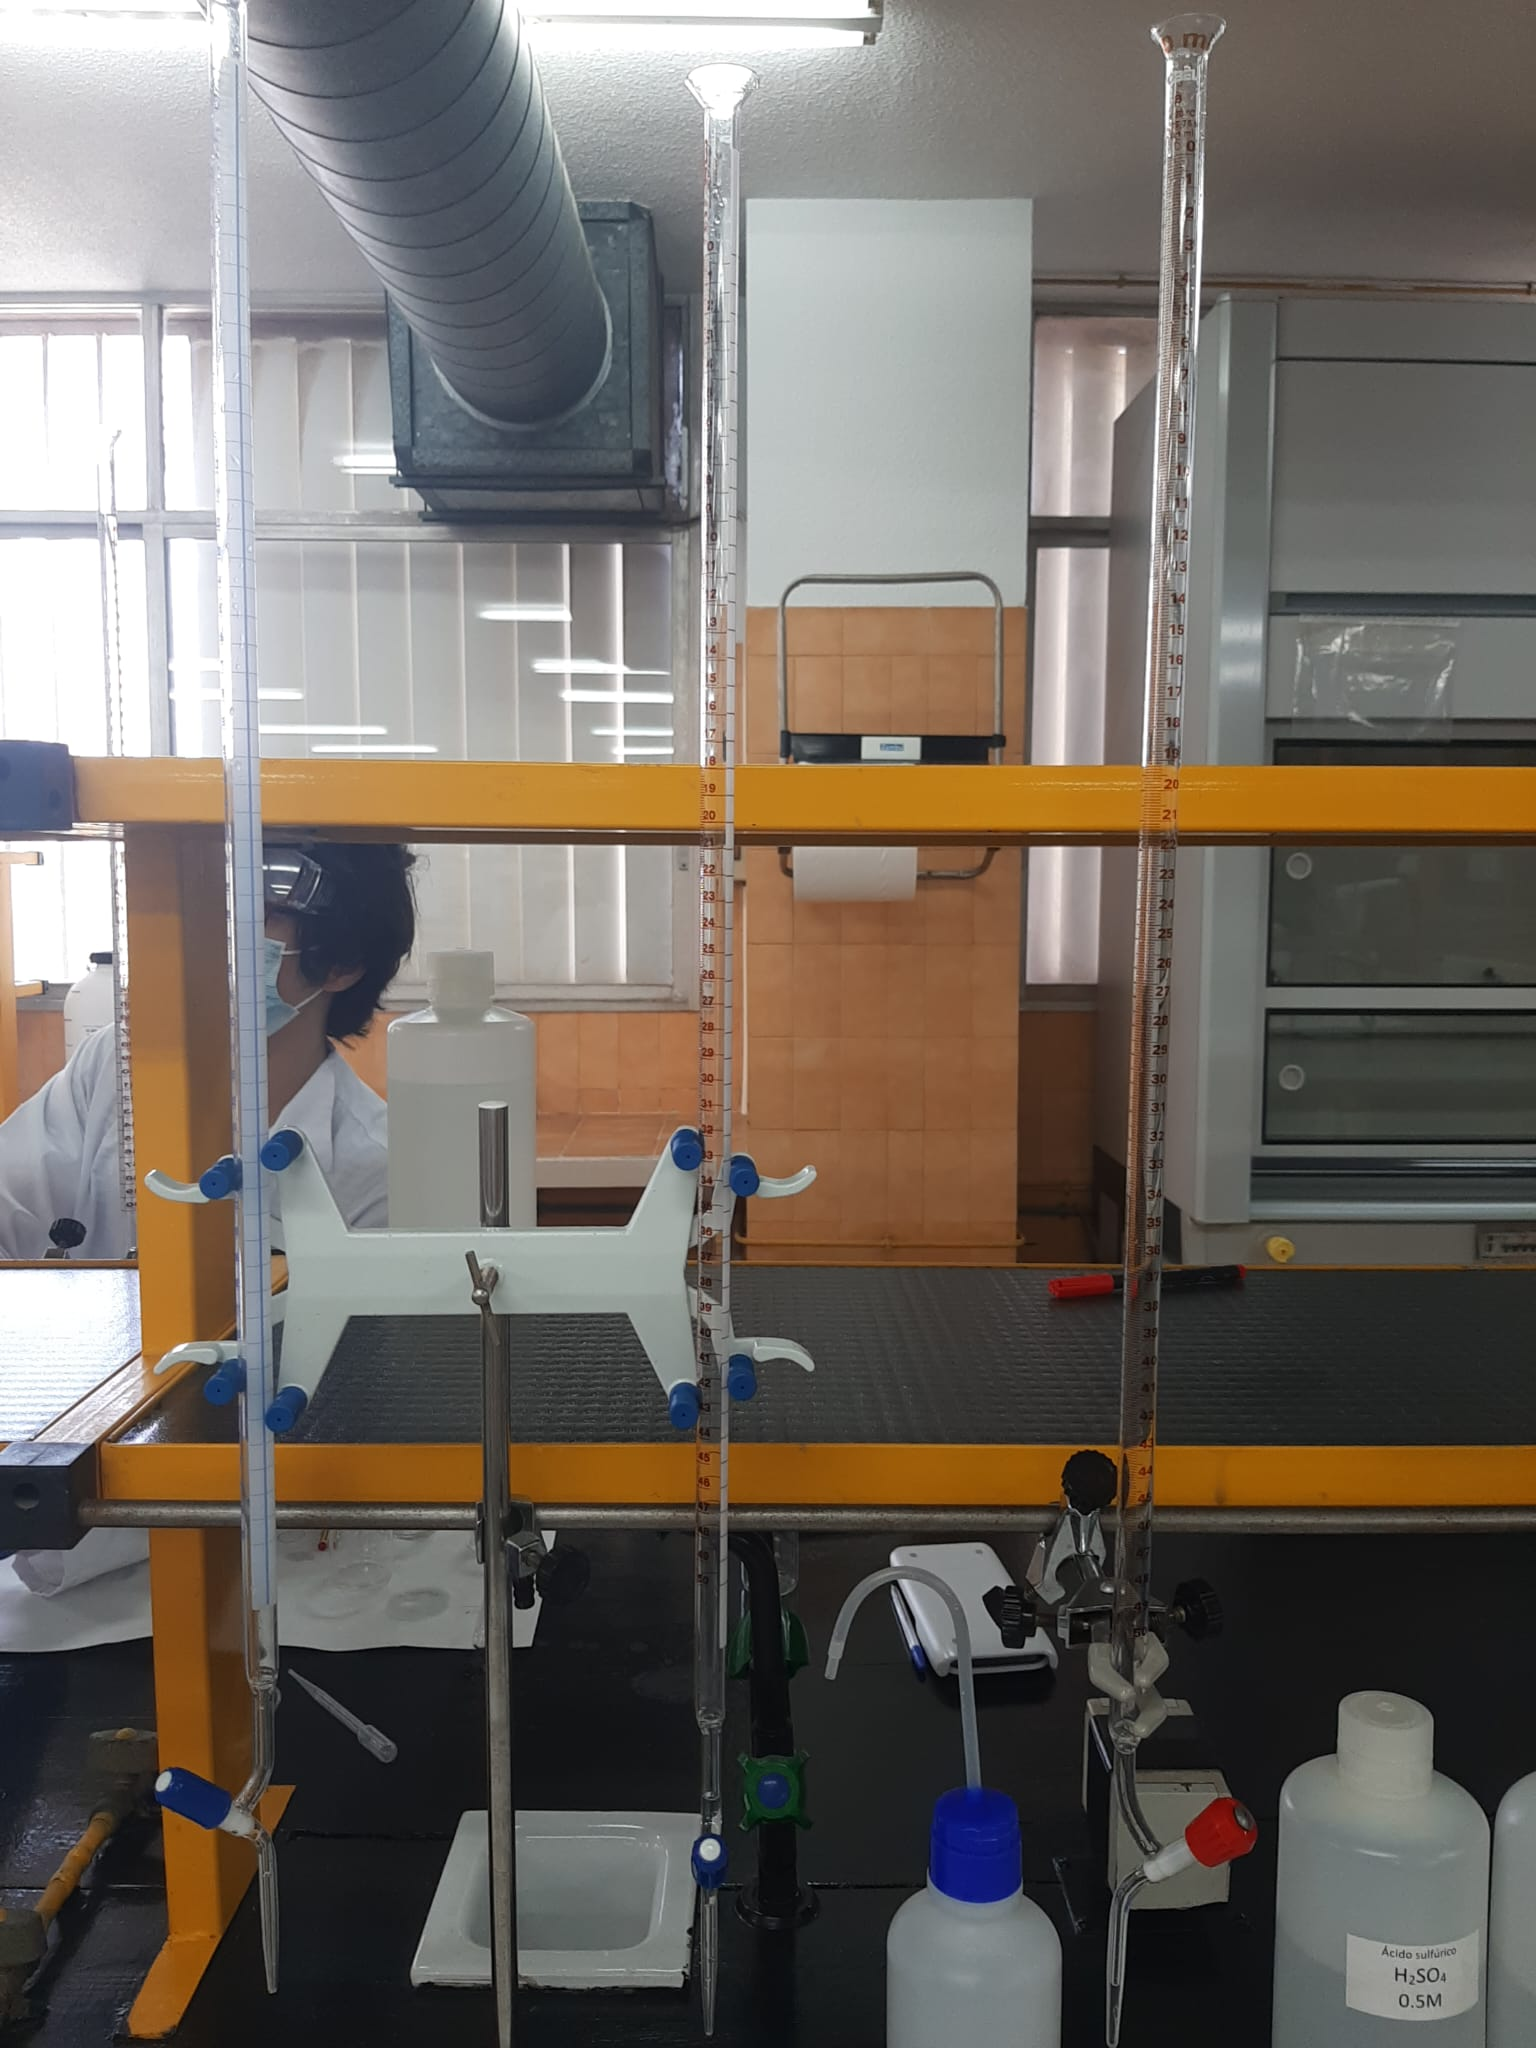
\includegraphics[scale = 0.093]{prac7/Buretas.jpeg}
    \hspace*{-3cm}
    \caption{Material utilizado a lo largo de la práctica}
    \vspace{-2cm}
\end{figure}
\clearpage

\section{Procedimiento}
\vspace{0.2cm}
\noindent Llenaremos las 3 buretas, la primera con agua destilada (\ce{H2O}), otra con ácido sulfúrico (\ce{H2SO4}) $0.5 M$ y la última con tiosulfato de sodio (\ce{Na2S2O3}) $0.3 M$. Numeraremos los vasos de precipitados que se nos dan y, ayudándonos de las buretas, llenaremos cada vaso de precipitados con las cantidades que se indican en la siguiente tabla.

\vspace{0.6cm}
\begin{table}[H]
\centering
\begin{tabular}{ccc}
\rowcolor[HTML]{CBCEFB} 
{\color[HTML]{000000} Número de Vaso} & {\color[HTML]{000000} Volúmen de \ce{Na2S2O3} ($ml$)} & {\color[HTML]{000000} Volúmen de \ce{H2O} ($ml$)} \\
\rowcolor[HTML]{ECF4FF} 
1 & 12 & 0 \\
2 & 8 & 4 \\
\rowcolor[HTML]{ECF4FF} 
3 & 6 & 6 \\
4 & 4 & 8 \\
\rowcolor[HTML]{ECF4FF} 
5 & 3 & 9 \\
6 & 2 & 10 \\
\rowcolor[HTML]{ECF4FF} 
7 & 1 & 11
\end{tabular}
\caption{volúmenes colocados en los vasos de precipitados}
\end{table}
\vspace{0.6cm}

\noindent Ahora, en un tubo de ensayo pondremos 12 $mL$ de la disolución de ácido sulfúrico (\ce{H2SO4}), que utilizaremos para verter en cada uno de los vasos, agitandolos bien y cronometrando el tiempo que esperamos hasta que empieza a aparecer turbidez. Este tiempo se anotará en una tabla, y se repetirá 3 veces el experimento para reducir el error humano del proceso.\\

\vspace{0.6cm}
\begin{table}[H]
\hspace*{-2cm}
\centering
\begin{tabular}{cccllclcc}
\cellcolor[HTML]{F6D594}{\color[HTML]{000000} Número de Vaso} &  & \cellcolor[HTML]{F6D594}Medida 1 - Tiempo ($s$) &  &  & \cellcolor[HTML]{F6D594}Medida 2 - Tiempo ($s$) &  &  & \cellcolor[HTML]{F6D594}Medida 3 - Tiempo ($s$) \\
\cellcolor[HTML]{EAEABE}1 &  & \cellcolor[HTML]{EAEABE}$8.38$ &  &  & \cellcolor[HTML]{EAEABE}$8.93$ &  &  & \cellcolor[HTML]{EAEABE}$8.80$ \\
2 &  & $12.21$ &  &  & $12.87$ &  &  & $12.13$ \\
\cellcolor[HTML]{EAEABE}3 &  & \cellcolor[HTML]{EAEABE}$17.83$ &  &  & \cellcolor[HTML]{EAEABE}$18.78$ &  &  & \cellcolor[HTML]{EAEABE}$16.34$ \\
4 &  & $24.55$ &  &  & $23.61$ &  &  & $22.26$ \\
\cellcolor[HTML]{EAEABE}5 &  & \cellcolor[HTML]{EAEABE}$31.75$ &  &  & \cellcolor[HTML]{EAEABE}$36.50$ &  &  & \cellcolor[HTML]{EAEABE}$33.59$ \\
6 &  & $52.46$ &  &  & $51.49$ &  &  & $48.53$ \\
\cellcolor[HTML]{EAEABE}7 &  & \cellcolor[HTML]{EAEABE}$108.96$ &  &  & \cellcolor[HTML]{EAEABE}$99.50$ &  &  & \cellcolor[HTML]{EAEABE}$104.06$
\end{tabular}
\caption{Resultados obtenidos a lo largo de la práctica}
\hspace*{-2cm}
\label{resultados7}
\end{table}
\clearpage

\section{Cuestiones}
\noindent\textcolor{BlueViolet}{\textbf{\textit{a) Calcule la concentración inicial de tiosulfato sódico $([A]_0)$ en cada vaso. Represente gráficamente $\log(\frac{1}{\Delta t})$ frente a $\log[A]_0$. Obtenga la ecuación de la recta a partir de la representación gráfica. Indique cuál es el orden de reacción experimental con respecto
al tiosulfato.}}}\\
\noindent Lo primero que haremos será reazliar una media de todas las medidas realizadas y descritas en el \ref{resultados7}
\begin{table}[H]
\centering
\begin{tabular}{cc}
\rowcolor[HTML]{F6D594} 
Número de Vaso & Tiempo (s) \\
\rowcolor[HTML]{EAEABE} 
1 & $08.70$ \\
2 & $12.40$ \\
\rowcolor[HTML]{EAEABE} 
3 & $17.65$ \\
4 & $23.47$ \\
\rowcolor[HTML]{EAEABE} 
5 & $33.95$ \\
6 & $50.83$ \\
\rowcolor[HTML]{EAEABE} 
\textbf{7} & $103.84$
\end{tabular}
\caption{Media de los resultados obtenidos}
\label{tab:my-table}
\end{table}
\noindent Ahora procedemos a calcular la concentración de tiosulfato sódico para cada vaso. Para hacerlo, usamos la expresión para calcular la concentración de una disolución:
\[M = \frac{\text{moles de soluto} (\si{n})}{\text{volumen de disolución} (\si{L})}\]
y por tanto,
\[\text{moles de soluto} (\si{n}) = M \cdot \text{volumen de la disolución} (\si{L})\]
\noindent Calculamos así los moles de soluto para cada vaso. Con ello y el volumen de agua añadido, calculamos la nueva concentración. Los resultados vienen representados en la tabla:
\begin{table}[H]
\centering
\begin{tabular}{ccc}
\rowcolor[HTML]{F6D594} 
Número de Vaso & Moles de soluto (\si{mol}) & Concentración (\si{M}) \\
\rowcolor[HTML]{EAEABE} 
1 & $3.6\cdot10^{-3}$ & $0.3$ \\
2 & $2.4\cdot10^{-3}$ & $0.2$ \\
\rowcolor[HTML]{EAEABE} 
3 & $1.8\cdot10^{-3}$ & $0.15$ \\
4 & $1.2\cdot10^{-3}$ & $0.1$ \\
\rowcolor[HTML]{EAEABE} 
5 & $9\cdot10^{-4}$ & $0.075$ \\
6 & $6\cdot10^{-4}$ & $0.05$ \\
\rowcolor[HTML]{EAEABE} 
7 & $3\cdot10^{-4}$ & $0.025$
\end{tabular}
\caption{Concentraciones}
\label{concentraao}
\end{table}
\clearpage

\noindent Una vez obtenidos los datos de las concentraciones inciales, vamos a representar $\log \frac{1}{\Delta \si{t}}$ frente a $\log [A]_0$ a partir de la expresión:
\[\log \frac{1}{\Delta \si{t}} = \log 1^{k'}\ - \ \log\Delta x\ +\ n_A\cdot\log [A]_0\]
\noindent Para ello primeramente calculamos los logaritmos que aparecen en la siguiente tabla:
\begin{table}[H]
\centering
\begin{tabular}{ccc}
\rowcolor[HTML]{F6D594} 
Número de Vaso & $\log \frac{1}{\Delta\si{t}}$ & $\log [A]_0$ \\
\rowcolor[HTML]{EAEABE} 
1 & $-2.16$ & $-1.20$ \\
2 & $-2.52$ & $-1.60$ \\
\rowcolor[HTML]{EAEABE} 
3 & $-2.87$ & $-1.90$ \\
4 & $-3.16$ & $-2.30$ \\
\rowcolor[HTML]{EAEABE} 
5 & $-3.52$ & $-2.59$ \\
6 & $-3.93$ & $-2.99$ \\
\rowcolor[HTML]{EAEABE} 
7 & $-4.64$ & $-3.69$
\end{tabular}
\caption{Logaritmos}
\label{logaritmos}
\end{table}

\begin{figure}[H]
    \centering
    \hspace*{-3cm}
        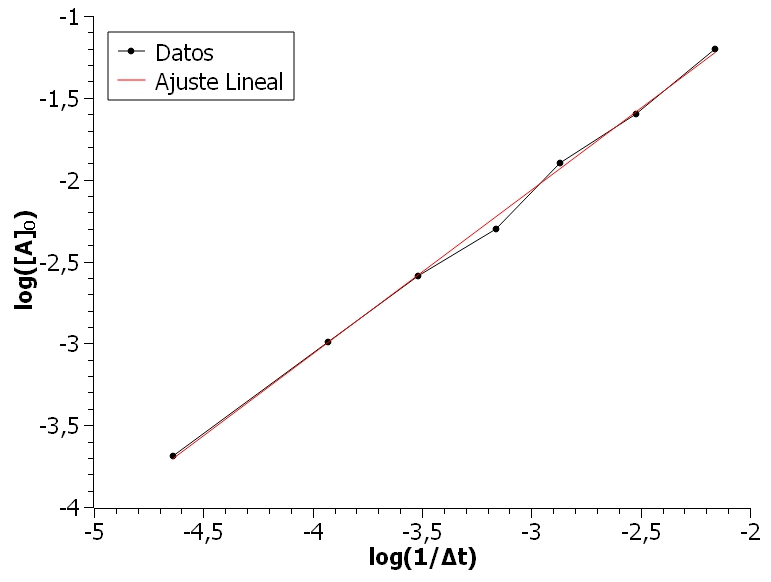
\includegraphics[scale = 0.5]{prac7/logaritmos.jpg}
    \hspace*{-3cm}
    \caption{Representación Gráfica}
\end{figure}

\noindent Del ajuste lineal obtenemos una ordenada en el origen de 0.93, siendo 1 el número natural más cercano y, por tanto, siendo 1 el orden de la reacción. La ecuación de la recta obtenida es $y = ax+b$, siendo $a = 1$ y $b = 0.93$.

% PRÁCTICA 8
\chapter[Práctica 8]{8. Espectroscopia y modelos moleculares}
\thispagestyle{empty}
\vspace{1.5cm}
\begin{figure}[h]
    \centering
    \hspace*{-0.2cm}
    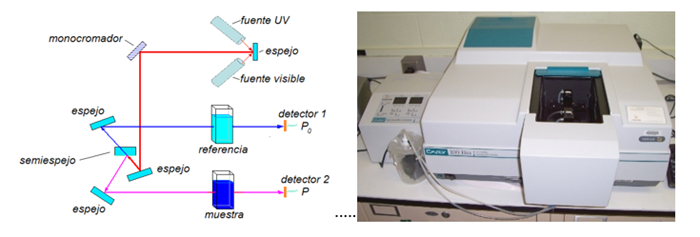
\includegraphics[width=1.1\textwidth]{fotos/espectrofotometro_uv_vis.png}
    \hspace*{-0.4cm}
\end{figure}
\section{Introducción}
\noindent La espectroscopia es el estudio de la interacción entre la radiación electromagnética y la materia, con absorción o emisión de energía radiante. En la primera parte de la práctica tendremos como finalidad medir la absorbancia de ambas muestras mediante un espectrofotómetro. El dispositivo que vamos a usar nos dará directamente la absorbancia, aunque también se puede calcular con:

\[A = \epsilon\cdot{l}\cdot{c}\]

\vspace{0.2cm}

\noindent donde $A$ será la absorbancia, $\epsilon$ el coeficiente de absorción molar, $l$ la longitud (= 1cm) y $c$ la concentración.

\noindent Aunque por la ley de Lambert Beer, la absorción vendrá dada por: $A = -log(T)$

\vspace{0.1cm}

%%%%%%%%VEEERRR

\noindent En la segunda parte formaremos moléculas de los principales grupos y las nombraremos.

\section{Inventario}
\noindent En esta práctica contamos con:

\begin{multicols}{2}
    \begin{itemize}
        \item 4 tubos de ensayo
        \item 3 vasos de precipitados
        \item Un espectrofotómetro
        \item Un matraz aforado
        \item Azul bromotimol
        \item Remazol
        \item Blanco (\ce{H2SO4})
        \item Una propipeta
        \item Una pipeta graduada
    \end{itemize}
\end{multicols}

\begin{figure}[H]
    \centering
    \hspace*{-2.3cm}
        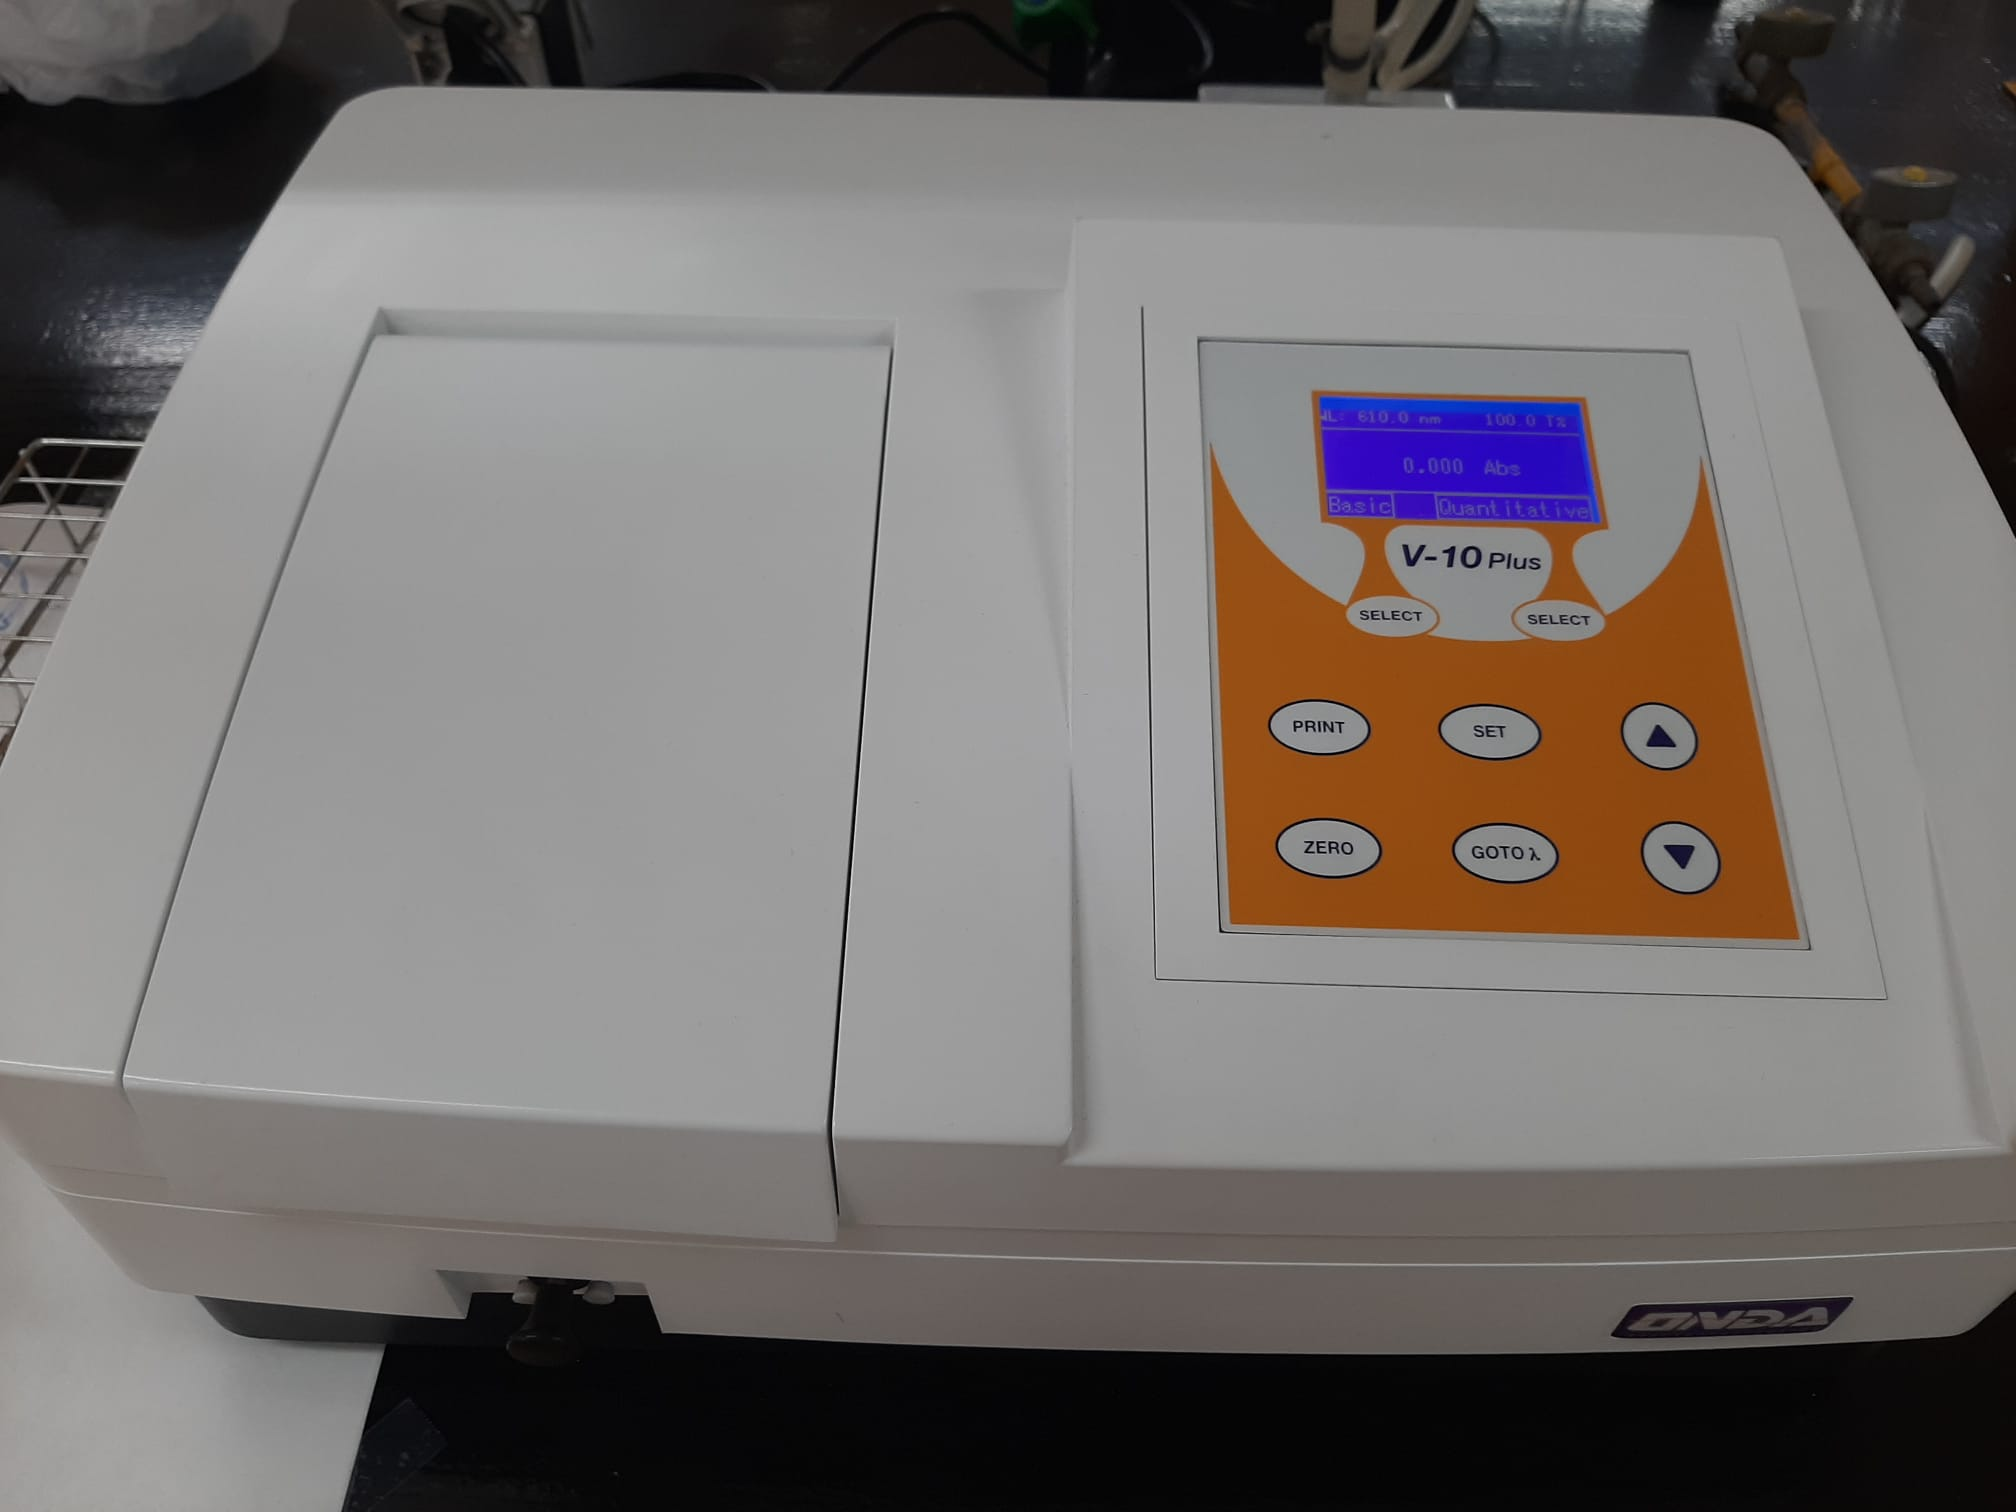
\includegraphics[scale = 0.07]{fotos/instru.jpeg}
        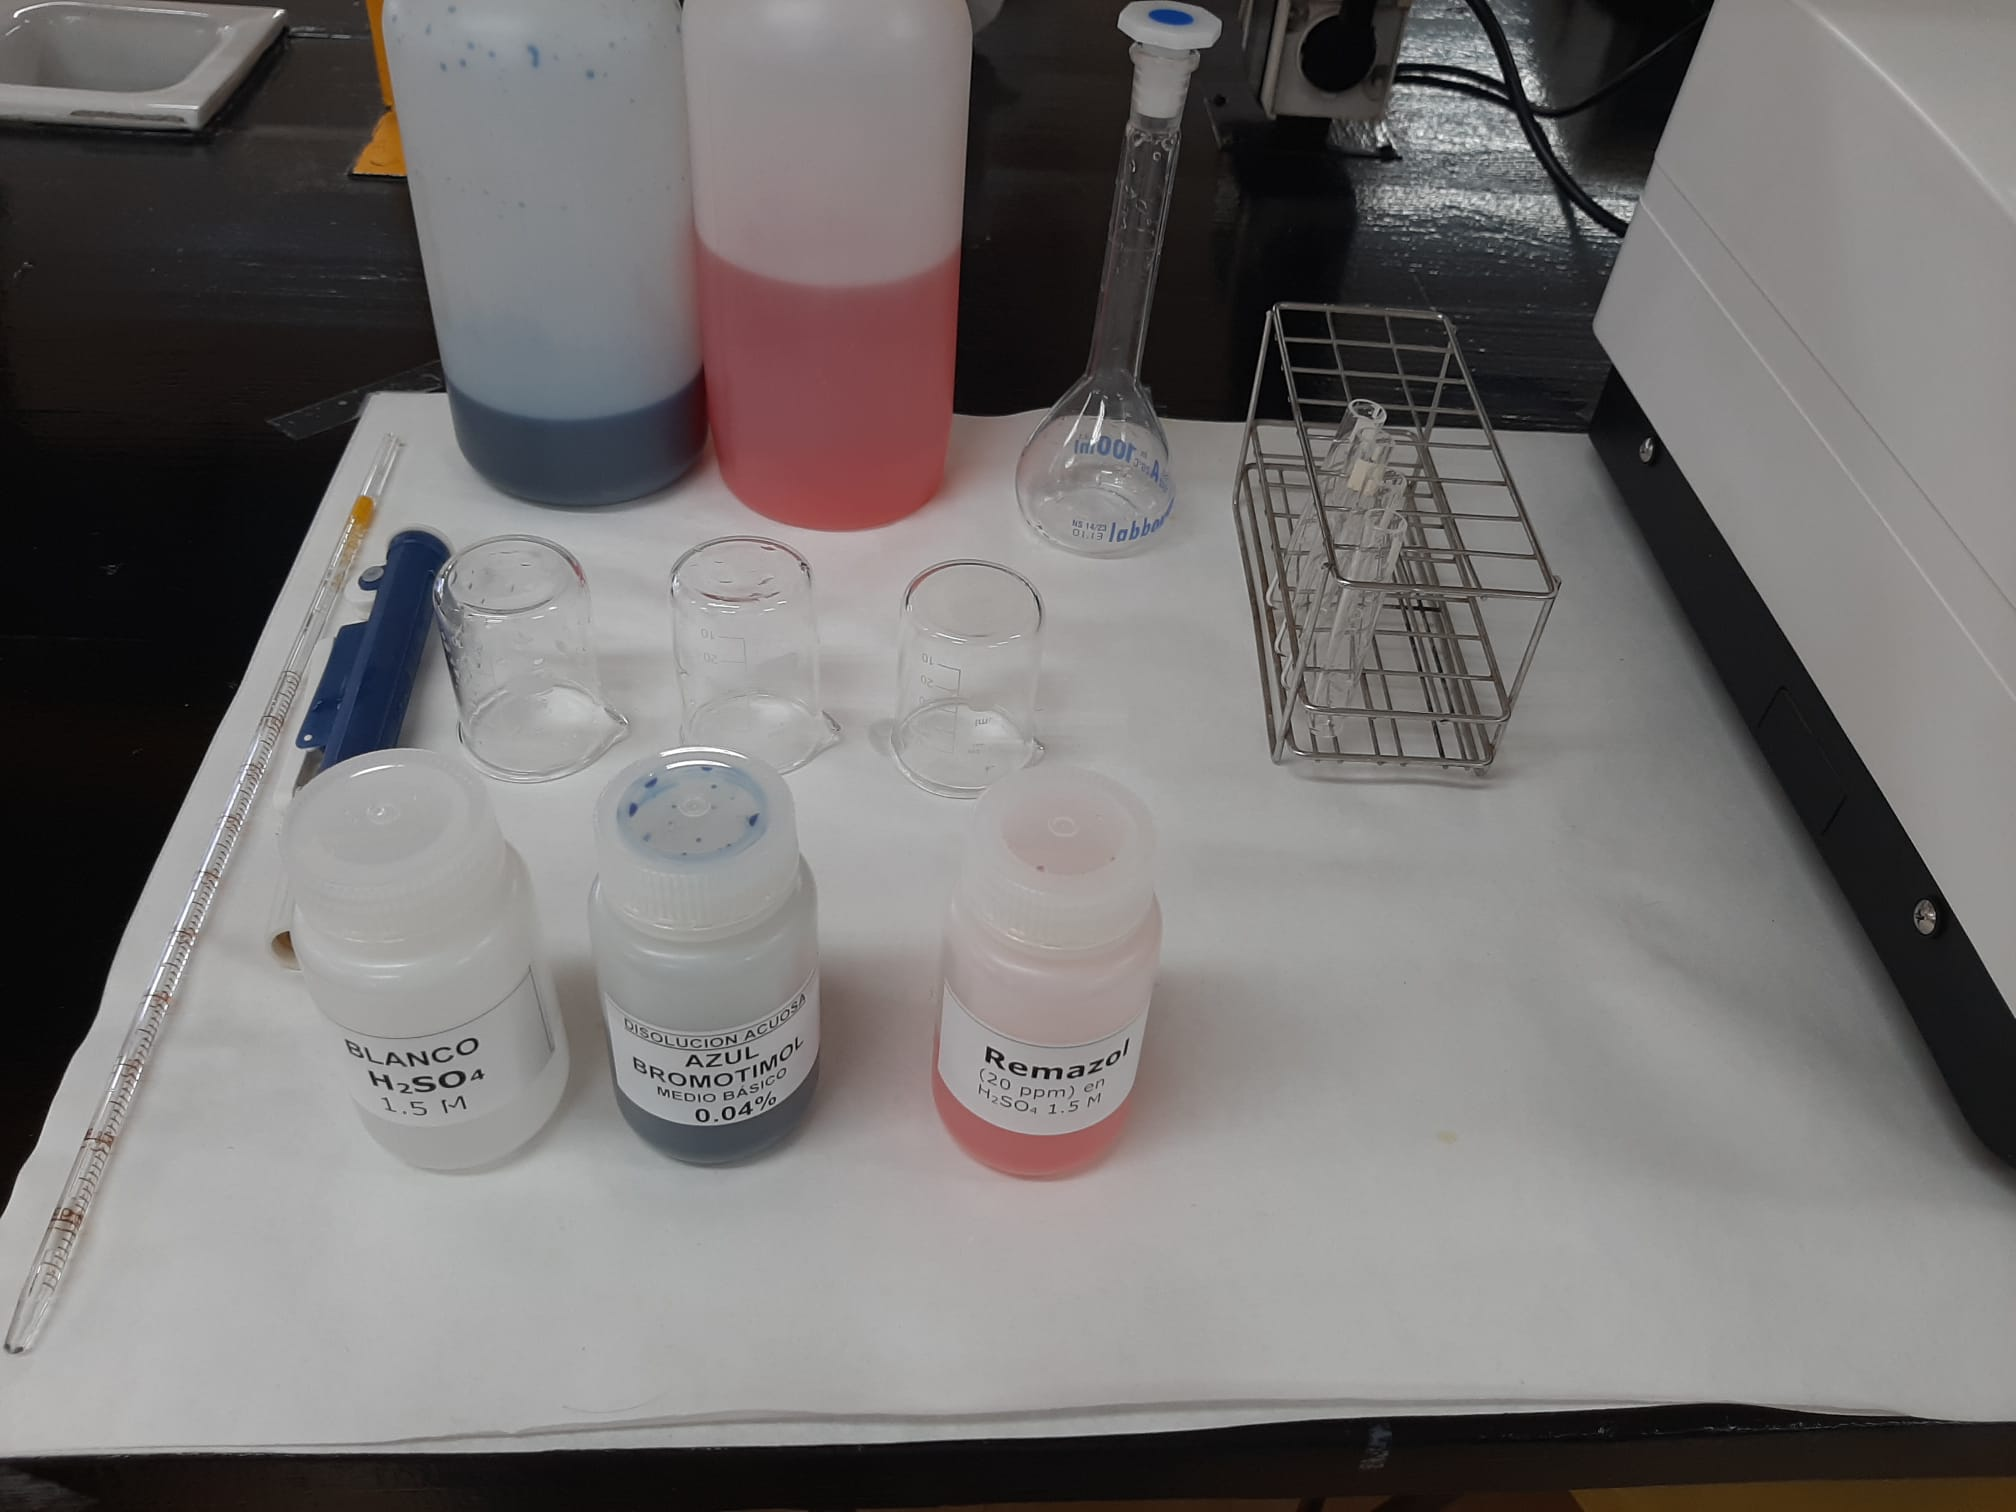
\includegraphics[scale = 0.07]{fotos/set8.jpeg}
    \hspace*{-2.3cm}
    \caption{Material utilizado, a la izquierda el espectrofotómetro y a la derecha el material usado}
\end{figure}
\clearpage

\section{Procedimiento}
\noindent En primer lugar, empezaremos la práctica preparando en cuatro cubetas, una con agua destilada, otra con azul bromotimol, otra con remazol y por último una con blanco(\ce{H2SO4}). Una vez hecho esto, nos dispondremos a empezar la práctica, teniendo que medir la absorbancia de cada muestra para determinadas longitudes de onda. Para ello, deberemos ajustar convenientemente la absorbancia del blanco a 0, y ya podremos medir la de la muestra.\\

%\vspace{0.2cm}

\noindent Cabe destacar que en la práctica había dos instrumentos distintos, uno más moderno y otro más antiguo. En nuestro caso, tuvimos el privilegio de contar con el nuevo, ya que nos permitía poner el blanco y nuestra muestra junta, sin necesidad de evaluar a cada longitud de onda el blanco y sacarlo para poner la muestra; es decir, nosotros colocábamos ambas cubetas y sólo debíamos tirar de una especie de barra metálica, a continuación dejo una foto para que sea más gráfico.

\vspace{0.4cm}

\begin{figure}[H]
    \centering
    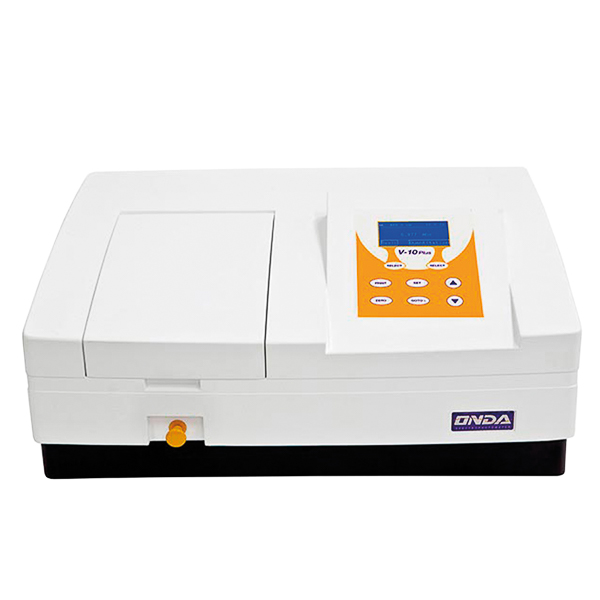
\includegraphics[scale = 0.2]{fotos/SPTR-V01-001.jpg}
    \caption{Espectrofotómetro visible, ONDA V-10 PLUS}
    \label{fig:cris}
\end{figure}

\vspace{0.4cm}


\noindent Primeramente, hacemos una dilución del Azul de bromotimol en un matraz aforado, con $1 mL$ de azul y $99 mL$ de agua (hasta llegar al máximo) y le agregamos una gota de de \ce{NaOH} $0.1M$.\\

\noindent Usaremos como blanco agua destilada y como muestra la disolución previamente explicada.\\

\noindent Una vez puestos los dos tubos de ensayo en el espectofotómetro, anotaremos la absorbancia para la diferentes longitudes de onda. Lo evaluaremos en el rango de 450 hasta 700 nanometros, aumentando la longitud de onda a razón de $10 nm$, y nos anotaremos en qué punto el valor de la absorbancia será mayor. Luego haremos una segunda pasada, donde abarcaremos un rango de -10nm y +10nm tomando como referencia el punto donde la absorbancia es mayor y mediremos dicho valor cambiando la longitud de onda de 2 en 2, para obtener así un resultado más preciso.\\


\noindent Una vez terminado lo anterior, cambiaremos los tubos de ensayo por blanco(\ce{H2SO4}) y la muestra de remazol. Haremos lo mismo que en el paso previo, solo que ahora el rango de la longitud de onda va de 400 a 600 nm. \\

\noindent Los datos obtenidos así como la gráfica de los datos lo veremos en el apartado de las cuestiones.



\vspace{0.6cm}
%%%%%%VEEEEEEEEERRR PTEE 2




\noindent \textit{2. Mediante el uso de modelos moleculares construya las moléculas de azul de bromotimol y remazol RB 133, e identifique los principales grupos funcionales y
estructuras orgánicas sencillas.}\\

\noindent Principales grupos funcionales: cada uno de los tres anillos aromáticos compone, junto a los grupos metilos y tertbutilo, el grupo timol, el nombre 'bromotimol'msurge de tener enlazado un Br.\\

\noindent A continuación, expongo unas fotografías de los distintos grupos y estructuras orgánicas que hemos reproducido en el laboratorio:


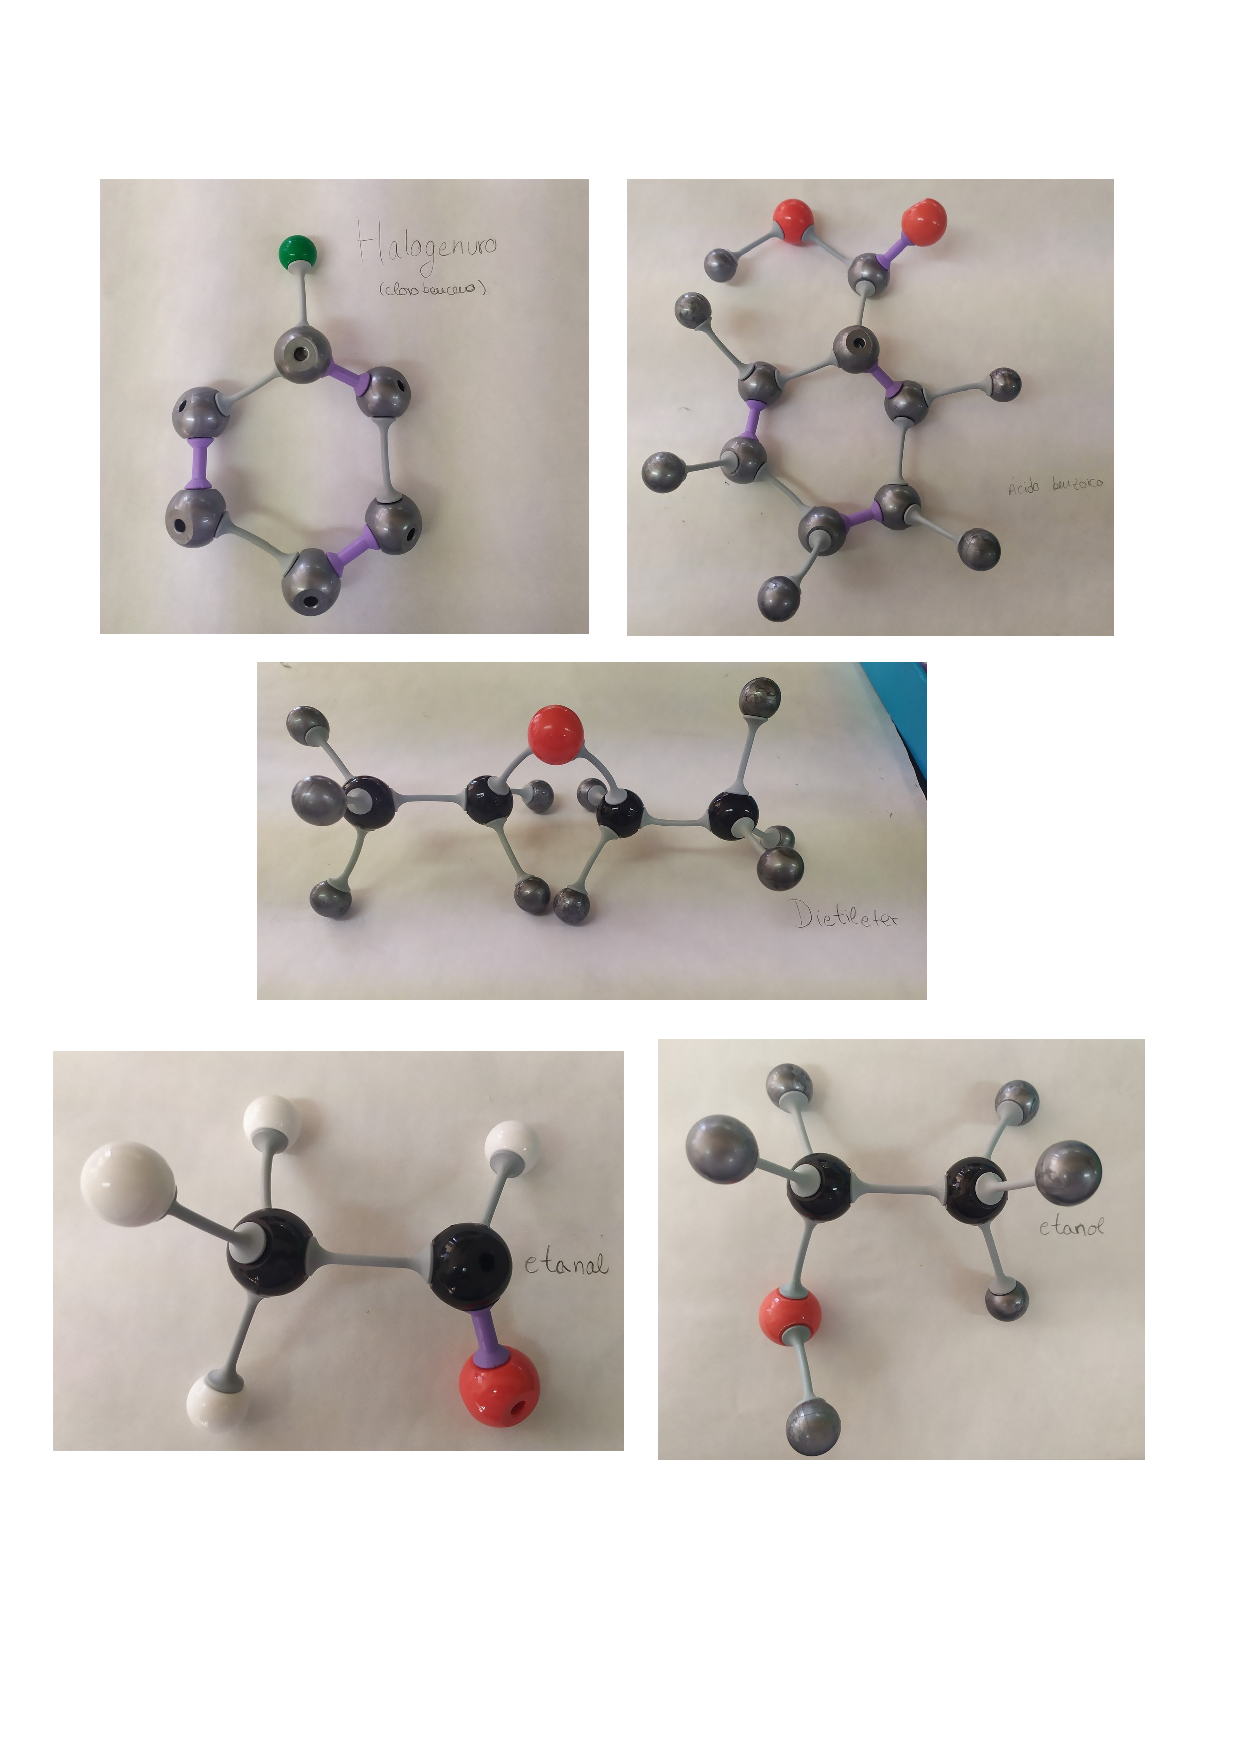
\includepdf[pages=-]{fotitos.pdf}



\clearpage

\section{Cuestiones}

\noindent\textcolor{BlueViolet}{\textbf{\textit{a) Determine el coeficiente de absorción molar del azul de bromotimol. Compare, si es posible, el resultado con el reportado en la bibliografía.}}}


\noindent El coeficiente de absorción puede expresarse por:

\[\epsilon = \frac{A}{l \cdot c}\]
 
\noindent siendo c la concentración, y la absorción la hemos calculado tal como hemos explicado en el procedimiento.

\vspace{0.4cm}

\begin{figure}[H]
    \centering
    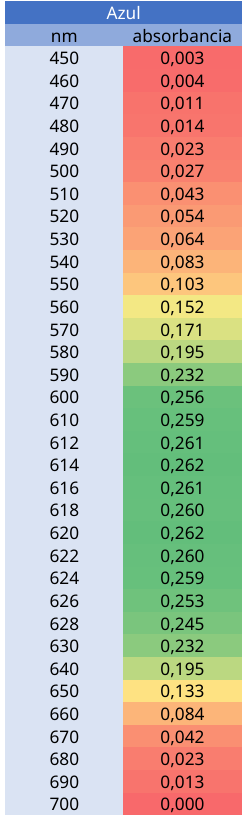
\includegraphics[scale = 0.333]{fotos/tabla azul.png}    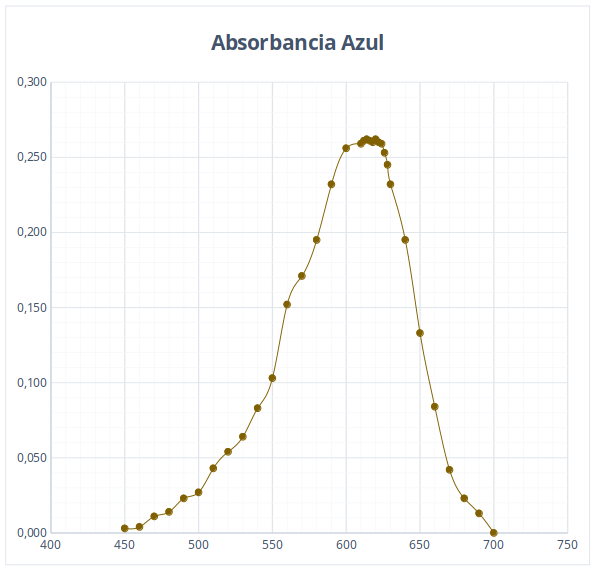
\includegraphics[scale = 0.433]{fotos/abs azul.png}
    \caption{Medidas tomadas y la correspondiente gráfica}
    \label{fig:cris}
\end{figure}

\vspace{0.4cm}

\noindent En la tabla, el color verde nos indica que hemos alcanzado el pico y por ello medimos para longitudes de onda que difieren de dos nanometros.

\noindent En esta gráfica podemos observar como $\epsilon$ varía con la longitud de onda de la luz, siendo este el gráfico del espectro de absorción. \\

\noindent A partir de estos datos, tomando el máximo valor de la gráfica podemos calcular el coeficiente de absorción mediante $A = \epsilon\cdot{l}\cdot{[concentración]}$, despejando tenemos que $\epsilon = \frac{0.262}{0.01\cdot{1.3}\cdot 10^{-4}}$ = \underline{$2.02\cdot{10^{5}}$}\\


\clearpage

\noindent\textcolor{BlueViolet}{\textbf{\textit{b) Determine el coeficiente de absorción molar del remazol RB 133. Compare, si es
posible, el resultado con el reportado en la bibliografía.}}}\\


\noindent Este apartado es similar al anterior, pero en lugar de tratar con azul de bromotimol usamos remazol RB 133.\\

\vspace{0.4cm}

\begin{figure}[H]
    \centering
    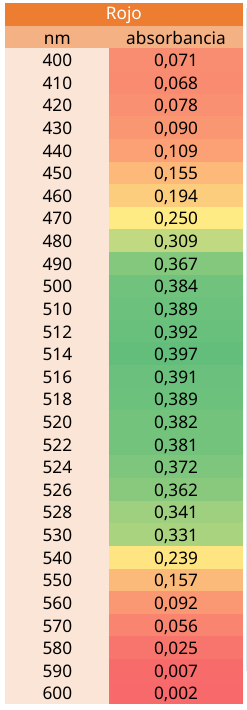
\includegraphics[scale = 0.333]{fotos/tabla rojo.png} 
    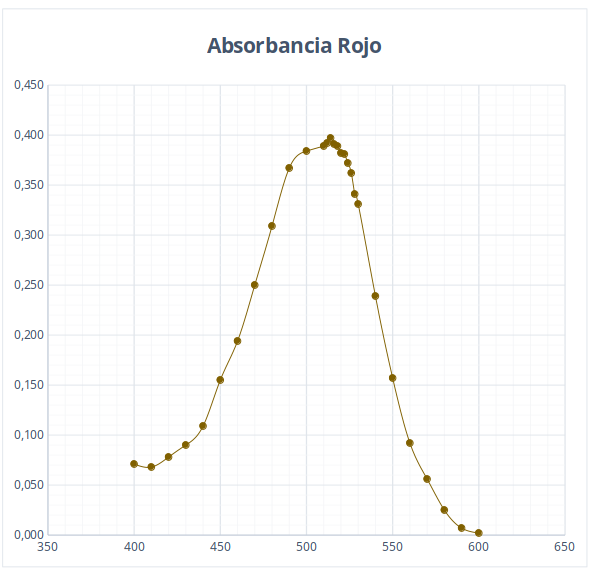
\includegraphics[scale = 0.433]{fotos/abs rojo.png}   
    \caption{Medidas tomadas y la correspondiente gráfica}
    \label{fig:cris}
\end{figure}

\vspace{0.4cm}

\noindent En esta gráfica podemos observar como la variación de la absorbancia en función de la longitud de onda de la luz, siendo este el gráfico del espectro de absorción, al igual que hemos visto en \textit{a)}. Además, a modo de aclaración, el color verde nos indica que hemos alcanzado el pico y es por eso que pasamos a medir la absorción para longitudes de onda que difieren en dos nanometros.\\


\noindent A partir de estos datos, tomando el máximo valor de la gráfica podemos calcular el coeficiente de absorción mediante $A = \epsilon\cdot{l}\cdot{[azul de bromotimol]}$, despejando tenemos que $\epsilon = \frac{0.397}{0.01\cdot{1}\cdot 10^{-4}}$ = \underline{$2.26\cdot{10^{5}}$}\\

\noindent No es posible comparar el resultado con el reportado en la bibliografía ya que no está, igual que para el apartado anterior. 


\clearpage

\noindent\textcolor{BlueViolet}{\textbf{\textit{c) Del apartado 2 del procedimiento, nombre las moléculas orgánicas de acuerdo con la nomenclatura de química orgánica.}}}\\


\noindent A continuación desarrollo una tabla en la que se encuentran formulados los compuestos de los que hay imágenes en la parte dos de la práctica:\\

\begin{table}[H]
\centering
\begin{tabular}{|l|c|}
\hline
\textbf{Nombre}                   & \textbf{Fórmula} \\ \hline
Halogenuro: clorobenceno          &         $C_6H_5Cl$            \\ \hline
Éter: dietiléter                  &         $(C_2H_5)_2O$         \\ \hline
Alcohol: etanol                   &         $C_2H_5OH$         \\ \hline
Aldehído: etanal                  &         $C_2H_4O$         \\ \hline
Ácido carboxílico: ácido benzoico &         $C_7H_6O_2$         \\ \hline
Éster: acetato de etilo           &         $C_4H_8O_2$     \\ \hline
Amida primaria: propanamida       &         $C_3H_7NO$         \\ \hline
Ácido salicílico                  &         $C_7H_6O_3$         \\ \hline
Ácido acetilsalicílico            &         $C_9H_8O_4$         \\ \hline
Naftaleno                         &         $C_{10}H_8$         \\ \hline
Ciclohexano                       &         $C_6H_{12}$         \\ \hline
Ciclopropano                      &         $C_3H_6$         \\ \hline
Ciclobutano                       &         $C_4H_8$         \\ \hline
Etano                             &         $C_2H_6$         \\ \hline
Eteno                             &         $C_2H_4$         \\ \hline
Etino                             &         $C_2H_2$         \\ \hline
Tiofeno                           &         $C_4H_4S$         \\ \hline
Sulfóxido de tiofeno              &         $C_4H_4SO$         \\ \hline
Sulfona de tiofeno                &         $C_4H_4SO_2$         \\ \hline
\end{tabular}
\end{table}

\vspace{0.3cm}

\noindent En esta tabla podemos diferenciar 4 grupos: del halogenuro al naftaleno pertenecen al \textbf{benceno y sus derivados}; los ciclo- pertenecen a los \textbf{compuestos cíclicos}; el etano, etano y etino a los \textbf{hidrocarburos} y los tres últimos pertenecen al \textbf{tiofeno y derivados}. Podemos observar que estos elementos son los que hemos puesto las fotografías en el apartado del desarrollo.










\end{document}